\documentclass[12pt, a4paper]{article}
\usepackage[utf8]{inputenc}
\usepackage{graphicx}
\usepackage[margin=2cm]{geometry}
\usepackage{amssymb}
\usepackage[table]{xcolor}
\usepackage{multirow}
%\usepackage{multicolumn}
\usepackage{array}
\newcommand{\checkbox}{$\square$}
\newcommand\fillin[1][3cm]{\makebox[#1]{\dotfill}}
%\newcolumntype{C}[1]{>{\centering\let\newline\\\arraybackslash\hspace{0pt}}m{#1}}
\newcommand{\PreserveBackslash}[1]{\let\temp=\\#1\let\\=\temp}
\newcolumntype{C}[1]{>{\PreserveBackslash\centering}p{#1}}
\newcolumntype{R}[1]{>{\PreserveBackslash\raggedleft}p{#1}}
\newcolumntype{L}[1]{>{\PreserveBackslash\raggedright}p{#1}}
\newcommand{\centered}[1]{\begin{tabular}{l} #1 \end{tabular}}
\begin{document}
\setcounter{page}{1}
\noindent {\Large \bf Ad/Soyadı: \dotfill}\\
\vspace*{0.8cm}
\begin{center}

\includegraphics[width=0.8\linewidth]{cebirlogo.png}


\includegraphics[width=0.25\linewidth]{bootstrap-logo.png}
 
\end{center}

\vspace*{0.2cm}


\begin{center}
{\Large \bf{Nesin Köyleri Cebir ve Programlama Yazokulu 2024 - Cebir}}

{\tiny Bootstrap is licensed under a Creative Commons 3.0 Unported License. Based on a work from
www.BootstrapWorld.org. Permissions beyond the scope of this license may be available at
contact@BootstrapWorld.org.

Türkçe versiyonu. Mehmet Gençer, Chris Stephenson ve diğer Nesin Köyleri Cebir ve Programlama Yazokulu öğretim takım üyeleri.

Lisans: Creative Commons 3.0 Unported License} 
\end{center}

\newpage
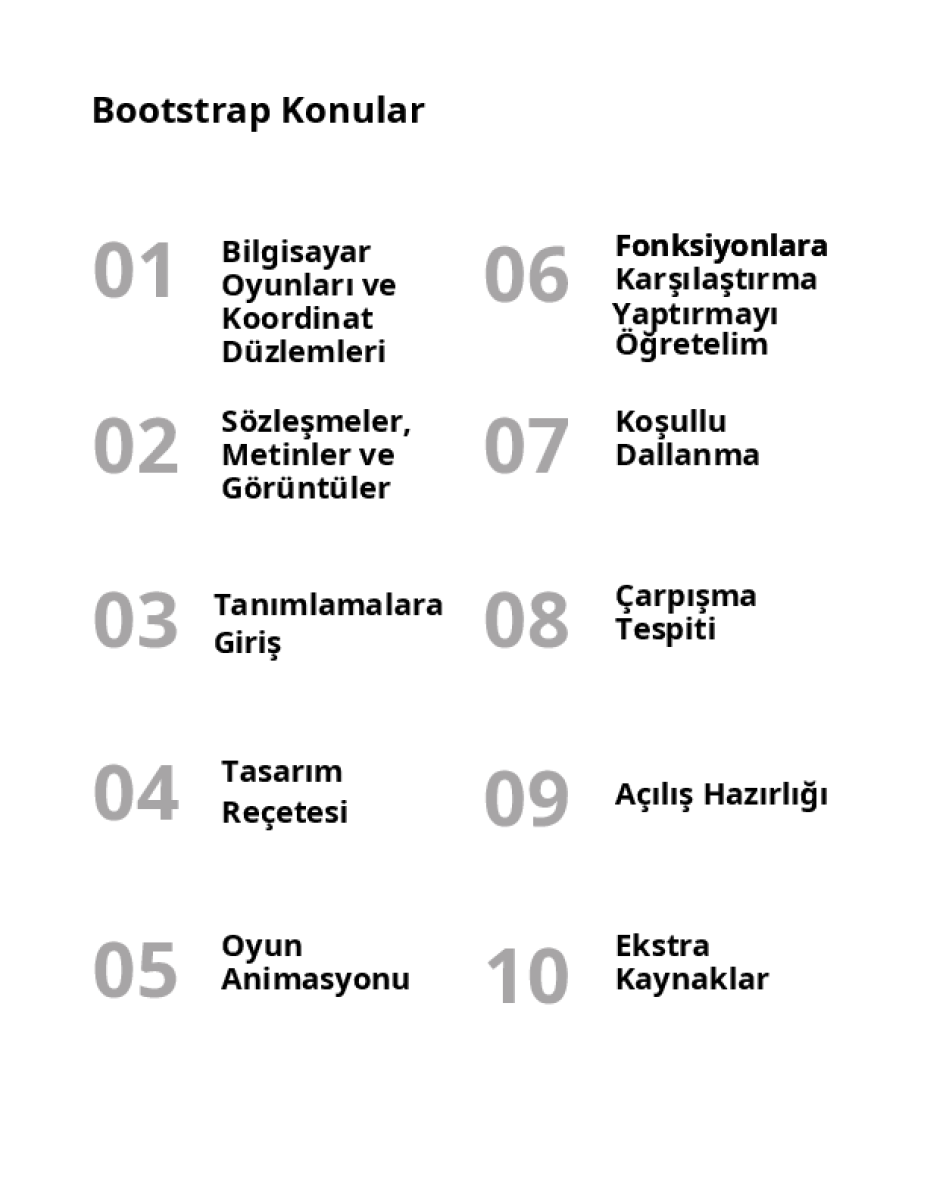
\includegraphics[width=1\linewidth]{cebirkapak-1.png}

\newpage
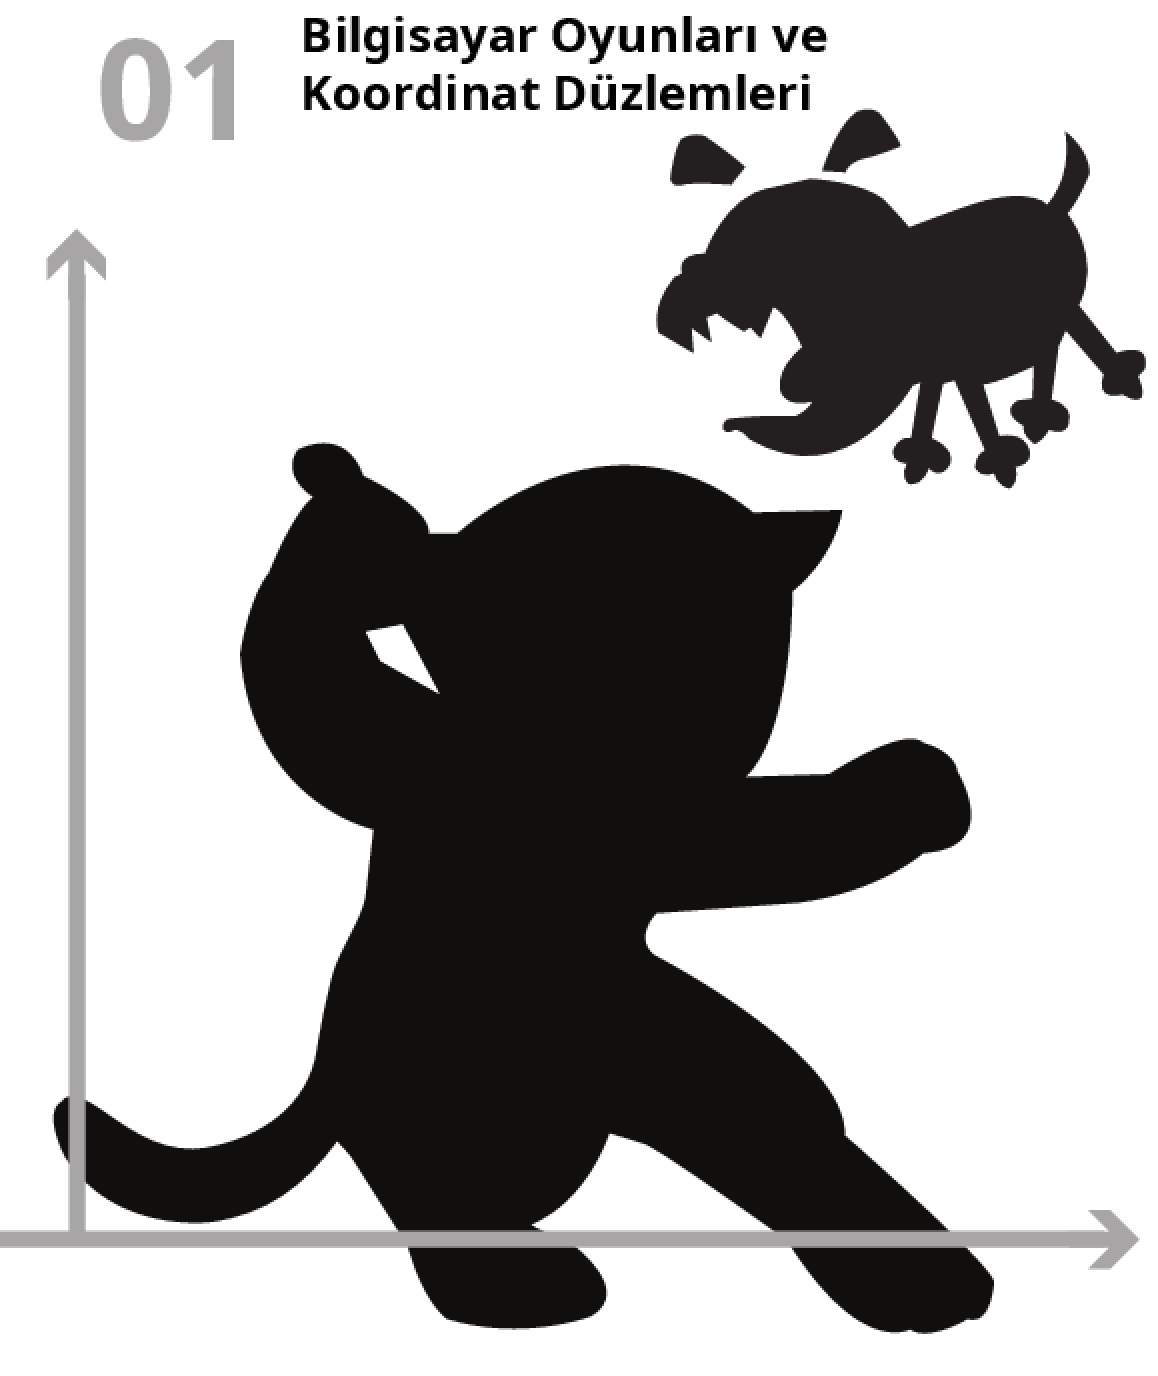
\includegraphics[width=1\linewidth]{cebir-bolum-01-000.png}
\newpage
%Cebir Bölüm 1 - 1
\section*{Ders 1}
\subsection*{Tersine Mühendislik: NinjaCat nasıl çalışır?}
\begin{tabular}{| p{4cm} | p{4cm} | p{8cm} |  }
\hline			
\bf Oyundaki nesne&\bf Ne değişiyor?&\bf Daha detaylıca...\\
\hline
\textit{bulut}&\textit{konum} &\textit{x koordinatı azalıyor, sola varınca sağa dönüyor} \\[2ex]
\hline  
 & &  \\[4ex]
\hline  
 & &  \\[4ex]
\hline  
 & &  \\[4ex]
\hline  
 & &  \\[4ex]
\hline  
 & &  \\[4ex]
\hline  
 & &  \\[4ex]
\hline  
 & &  \\[4ex]
\hline  
 & &  \\[4ex]
\hline  
 & &  \\[4ex]
\hline  
 & &  \\[4ex]
\hline  
 & &  \\[4ex]
\hline  
 & &  \\[4ex]
\hline  
 & &  \\[4ex]
\hline  
 & &  \\[4ex]
\hline
\end{tabular}


\newpage
%Cebir bölüm 1 - 2
\subsection*{Koordinatları Bulmak}
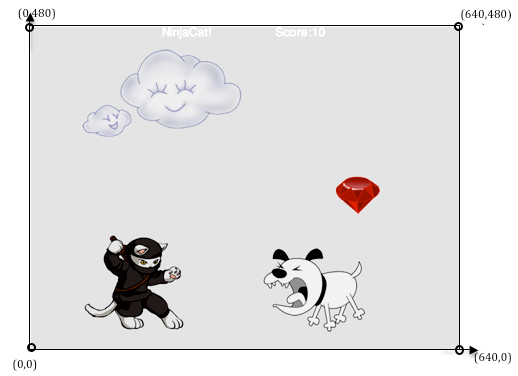
\includegraphics[width=1\linewidth]{ninja-sahne.png}

\subsection*{Oyundaki nesnelerin koordinatları} 
%\newline
\begin{tabular}{| p{8cm} | C{4cm} | C{4cm} |  }
\hline			
\centered{Oyundaki nesne}&x koordinatı&y koordinatı\\[4ex]
\hline  
Oyuncu (NinjaCat) için koordinatlar & &  \\[4ex]
\hline  
Tehlike (köpek) için koordinatlar: & &  \\[4ex]
\hline  
Hedef (yakut) için koordinatlar:  & &  \\[4ex]
\hline
\end{tabular}

\newpage
\section*{Kendi Video Oyunumuz}
 \vspace{4ex}
\noindent {\large \bf Geliştirici (adın) \dotfill}\\[4ex]
\begin{tabular}{| p{16.5cm} |  }
\hline
\begin{center}
\Large \bf Arka Plan\\
\end{center}\\
\hline
\end{tabular}
\vspace{4ex}\\
\noindent {\large \bf Oyunumuzun Ortamı : \dotfill}\\
(Örnek: Uzay? Çöl? Orman?)\\[4ex]
\begin{tabular}{| p{16.5cm} |  }
\hline
\begin{center}
\Large \bf Oyuncu\\
\end{center}\\
\hline
\end{tabular}
\vspace{4ex}\\

\noindent {\large \bf Oyuncu: \dotfill}\\
(Örnek: Tazmanya Canavarı)\\
\textit{Oyuncu sadece yukarı aşağı hareket edebilir}
\\[4ex]
\begin{tabular}{| p{16.5cm} |  }
\hline
\begin{center}
\Large \bf Hedef\\
\end{center}\\
\hline
\end{tabular}
\vspace{4ex}\\

\noindent {\large \bf Hedef: \dotfill}\\
(Örnek: Totem)\\
\textit{Hedef sadece sağa sola hareket edebilir}
\\[4ex]
\begin{tabular}{| p{16.5cm} |  }
\hline
\begin{center}
\Large \bf Tehlike\\
\end{center}\\
\hline
\end{tabular}
\vspace{4ex}\\

\noindent {\large \bf Tehlike: \dotfill}\\
(Örnek: Avcı)\\
\textit{Tehlike sadece sağa sola hareket edebilir}\\[4ex]
\newpage
\noindent{\Large \bf Değerlendirme Çemberi Pratiği}\\
\textit{Çarpma ve bölme sembollerini yazarken bilgisayar sembollerini kullanmayı unutma!}\\[2ex]
\begin{tabular}{| C{4cm} | C{6cm} | C{6cm} |  }
\hline
\bf Matematik&\bf Değerlendirme Cemberi&\bf Racket Kodu\\
\hline  
\begin{displaymath} 5 \times 10 \end{displaymath}  & &  \\[16ex]
\hline  
\begin{displaymath} 8 + (5 \times 10 ) \end{displaymath} & &  \\[16ex]
\hline  
\begin{displaymath} (8 + 2) - (5 \times 10 ) \end{displaymath}  & &  \\[16ex]
\hline  
\begin{displaymath} \frac{(5 \times 10 )}{(8-2)} \end{displaymath}   & &  \\[16ex]
\hline  
\end{tabular}
\newpage
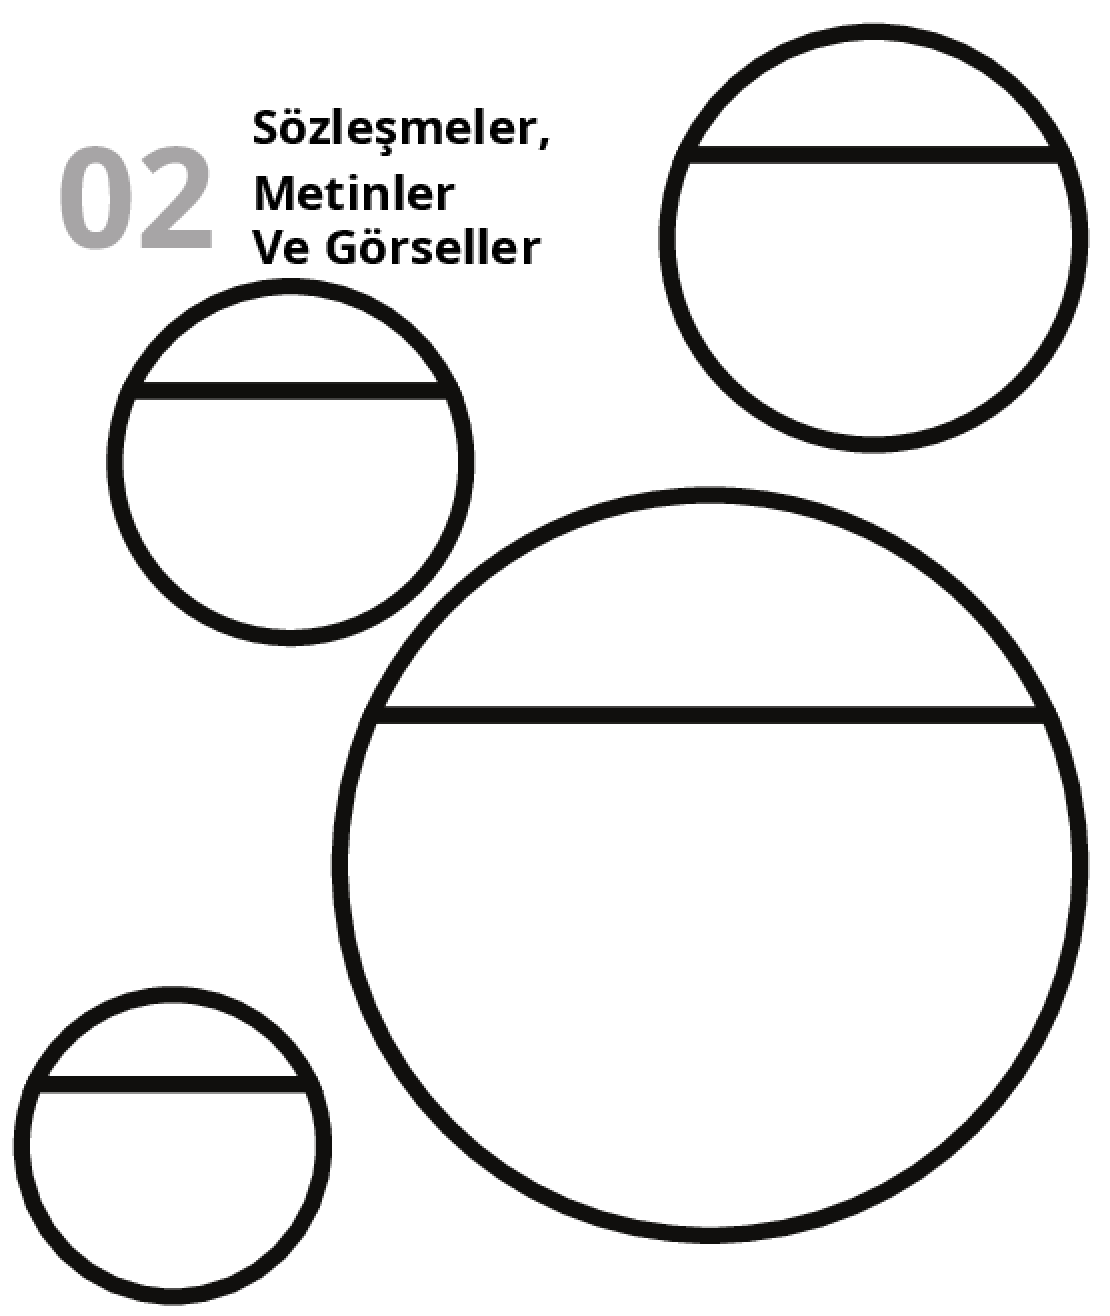
\includegraphics[width=1\linewidth]{cebir-bolum-02-000.png}
\newpage
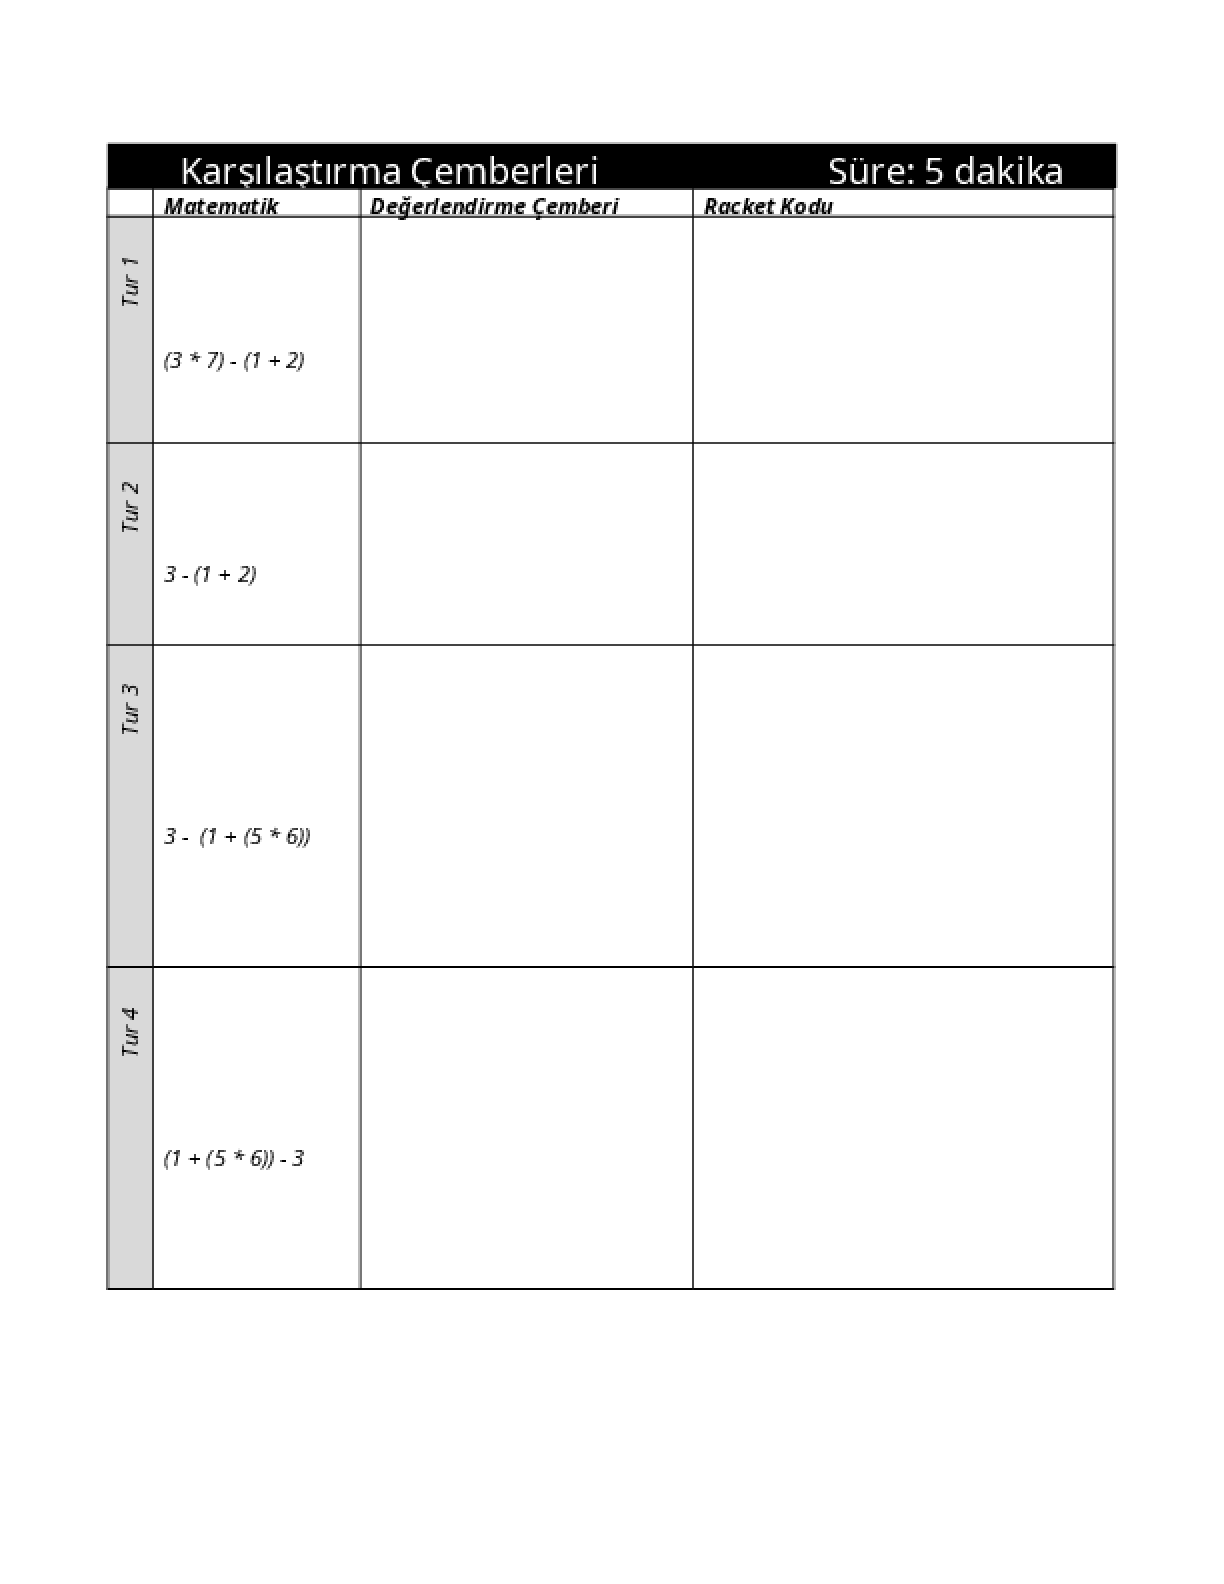
\includegraphics[width=1\linewidth]{cebirsplit-6.png}
\newpage
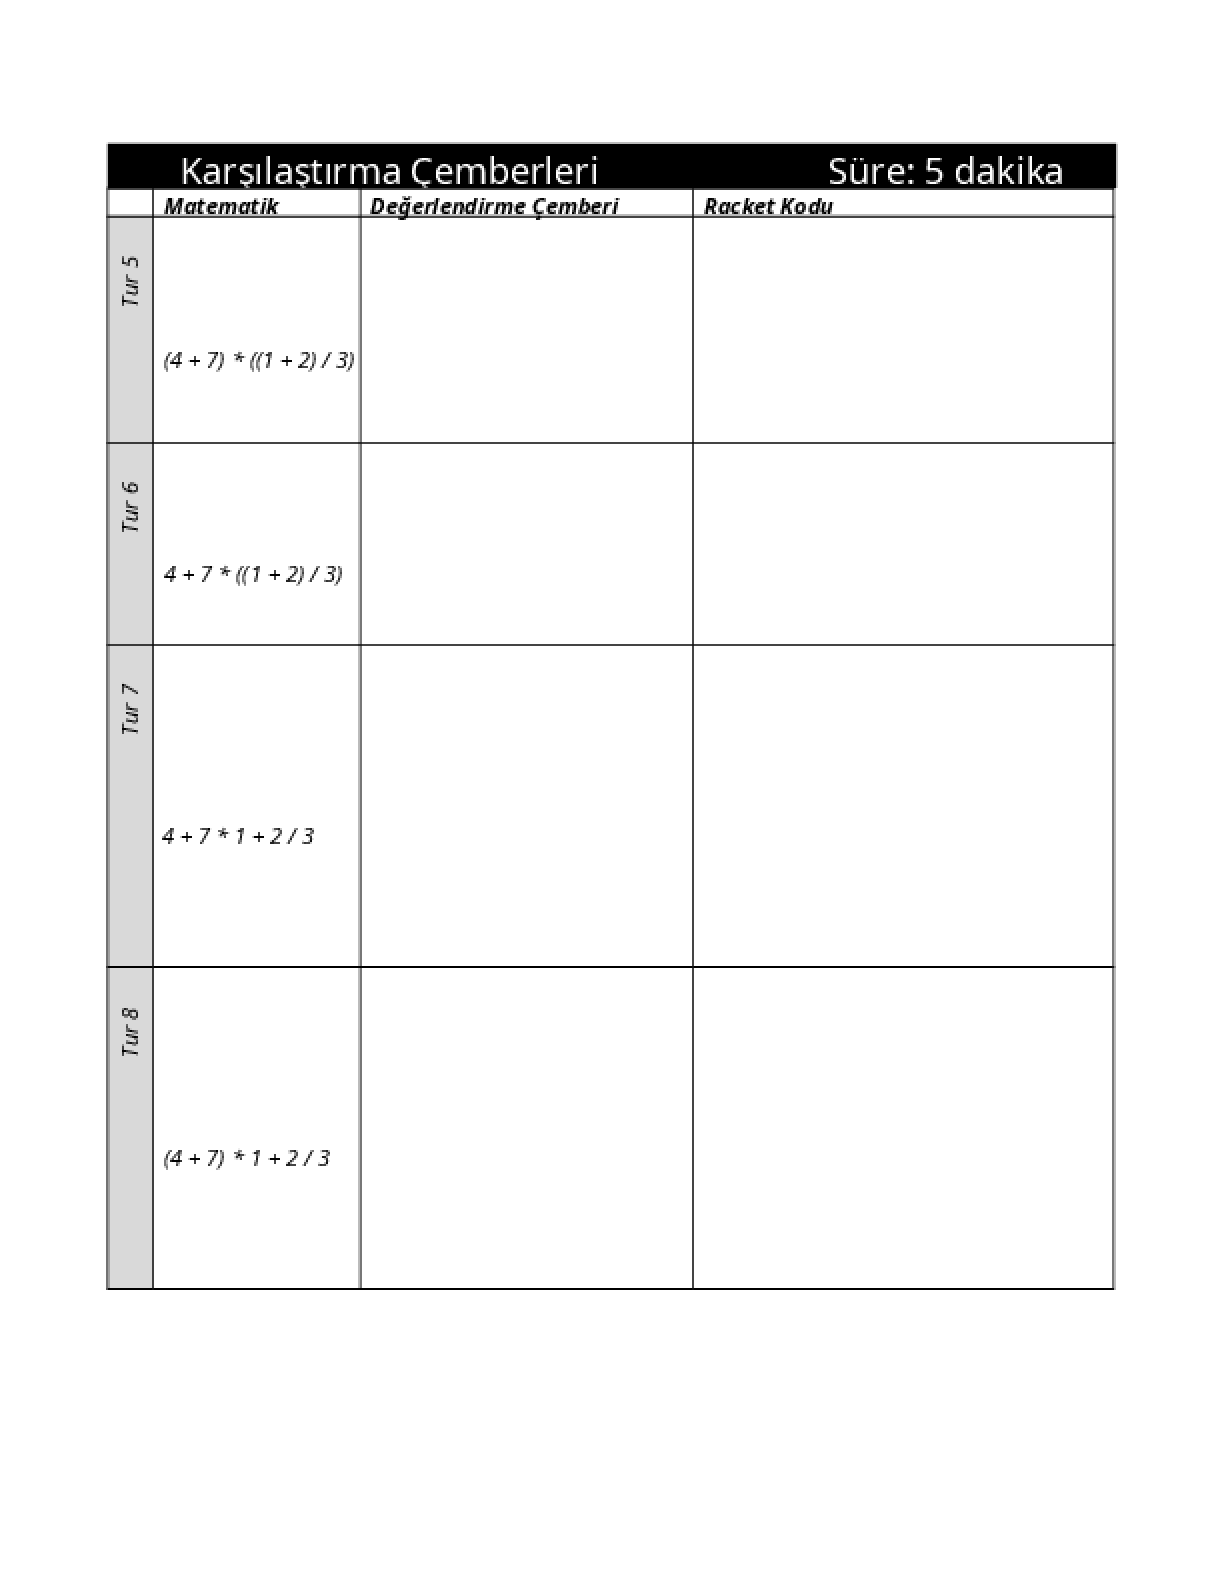
\includegraphics[width=1\linewidth]{cebirsplit-7.png}
\newpage
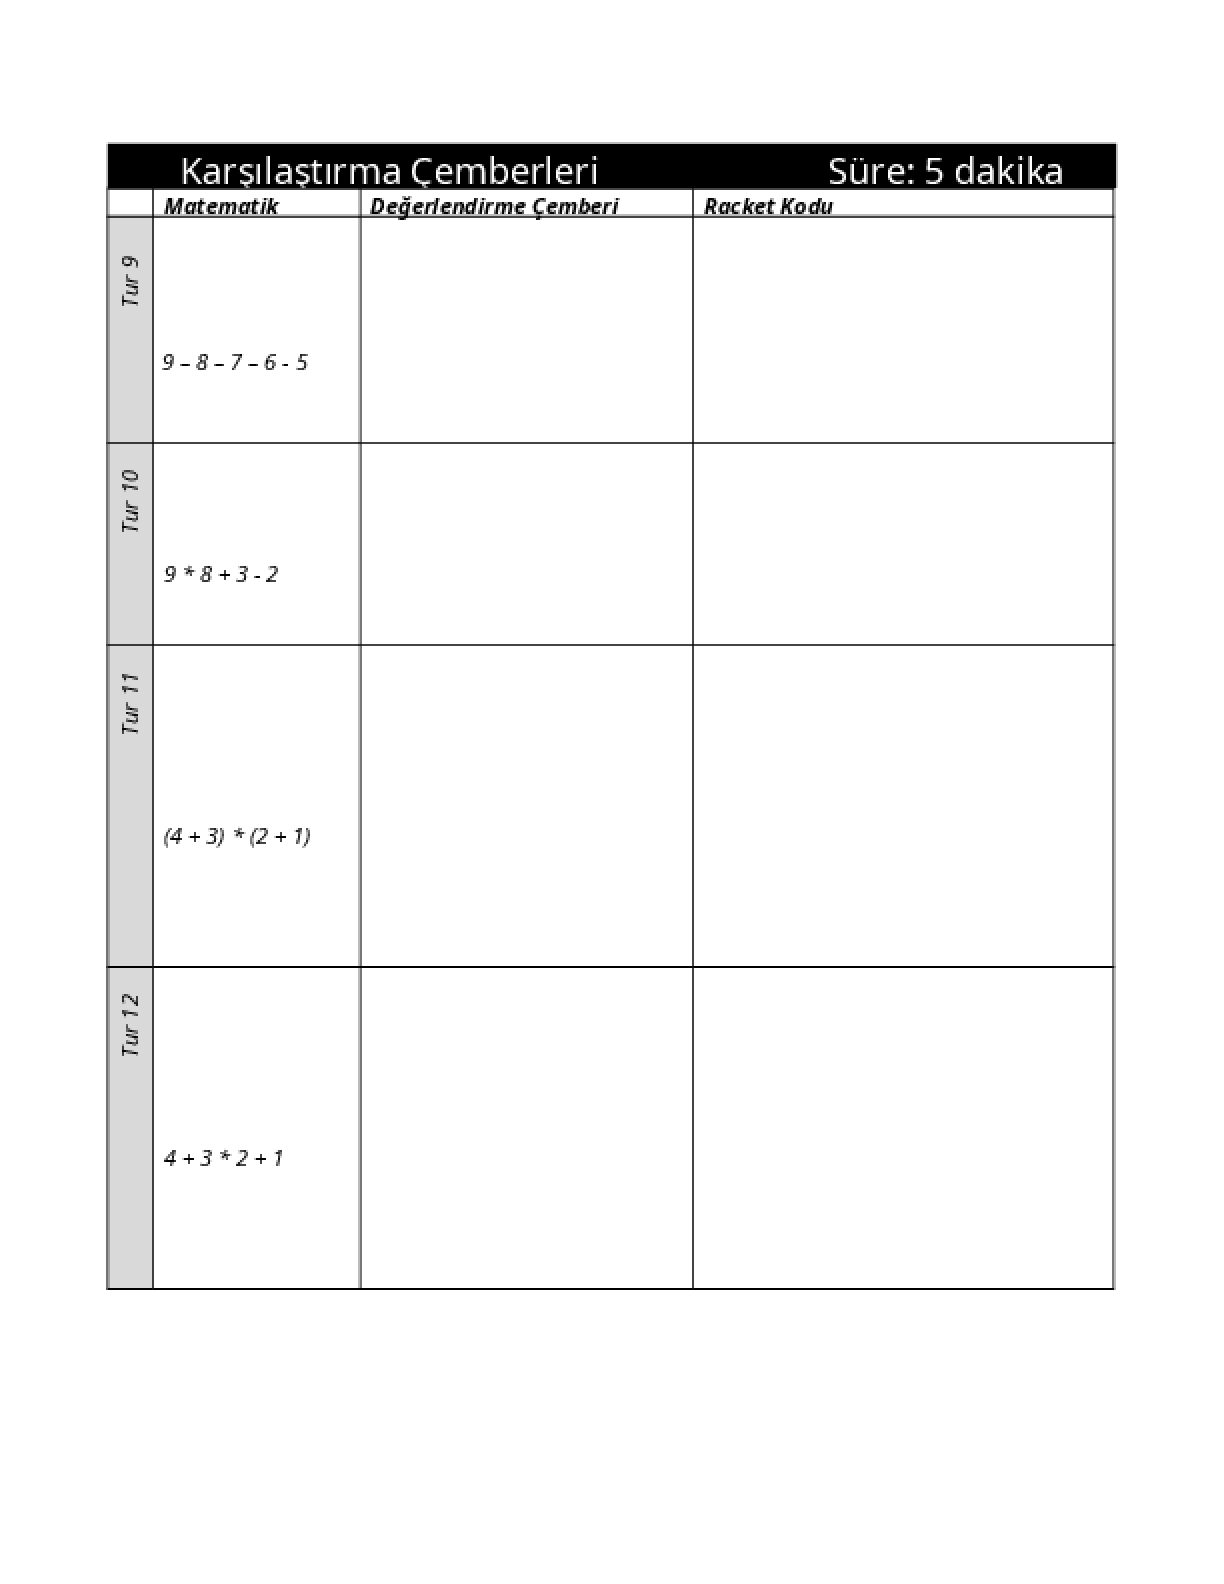
\includegraphics[width=1\linewidth]{cebirsplit-8.png}
\newpage
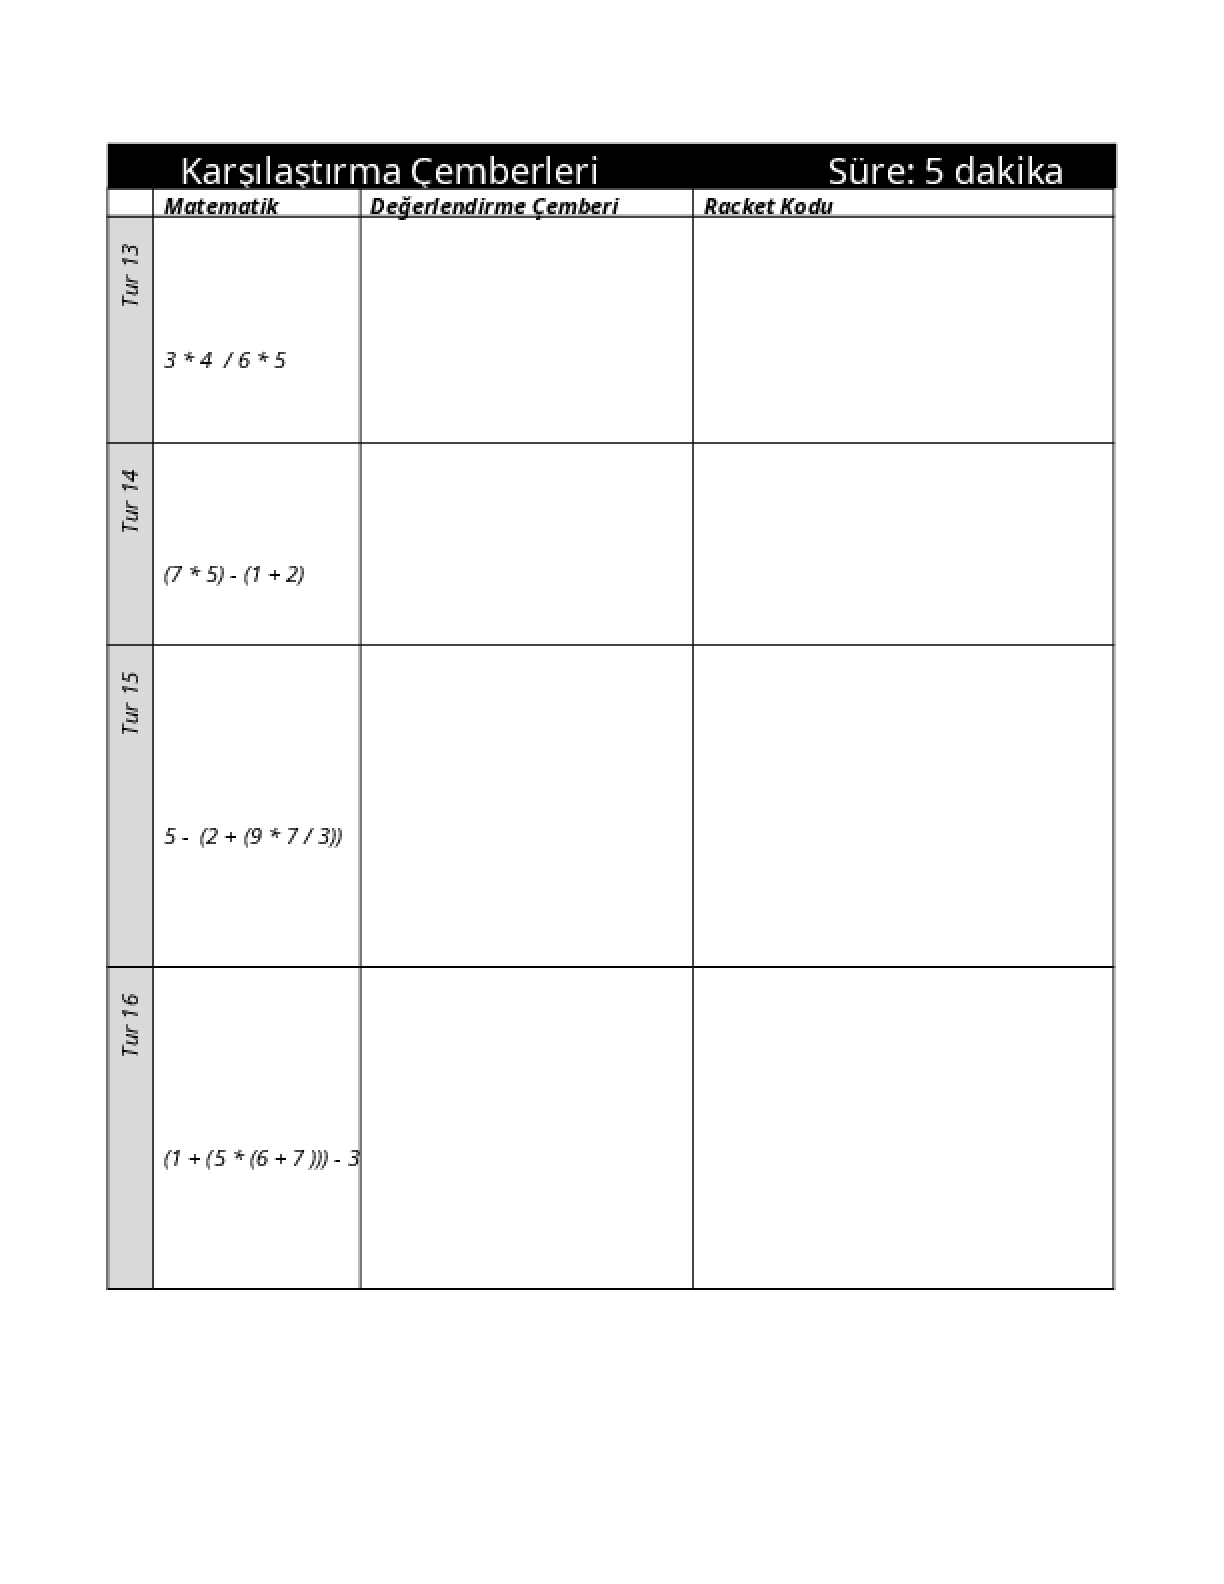
\includegraphics[width=1\linewidth]{cebirsplit-9.png}
\newpage
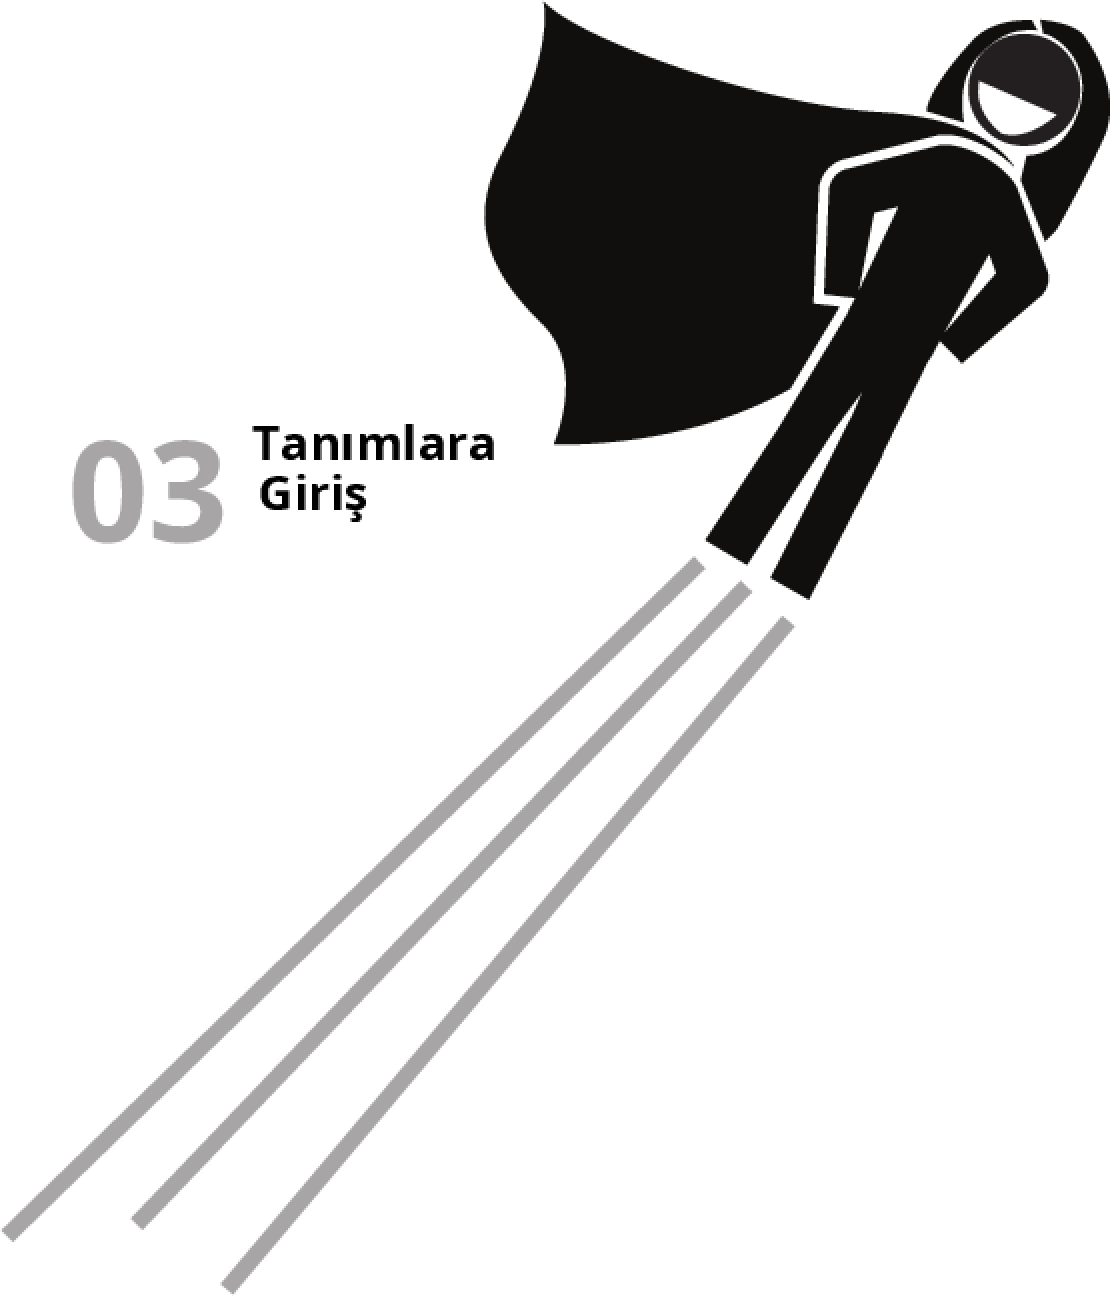
\includegraphics[width=1\linewidth]{cebir-bolum-03-000.png}
\newpage
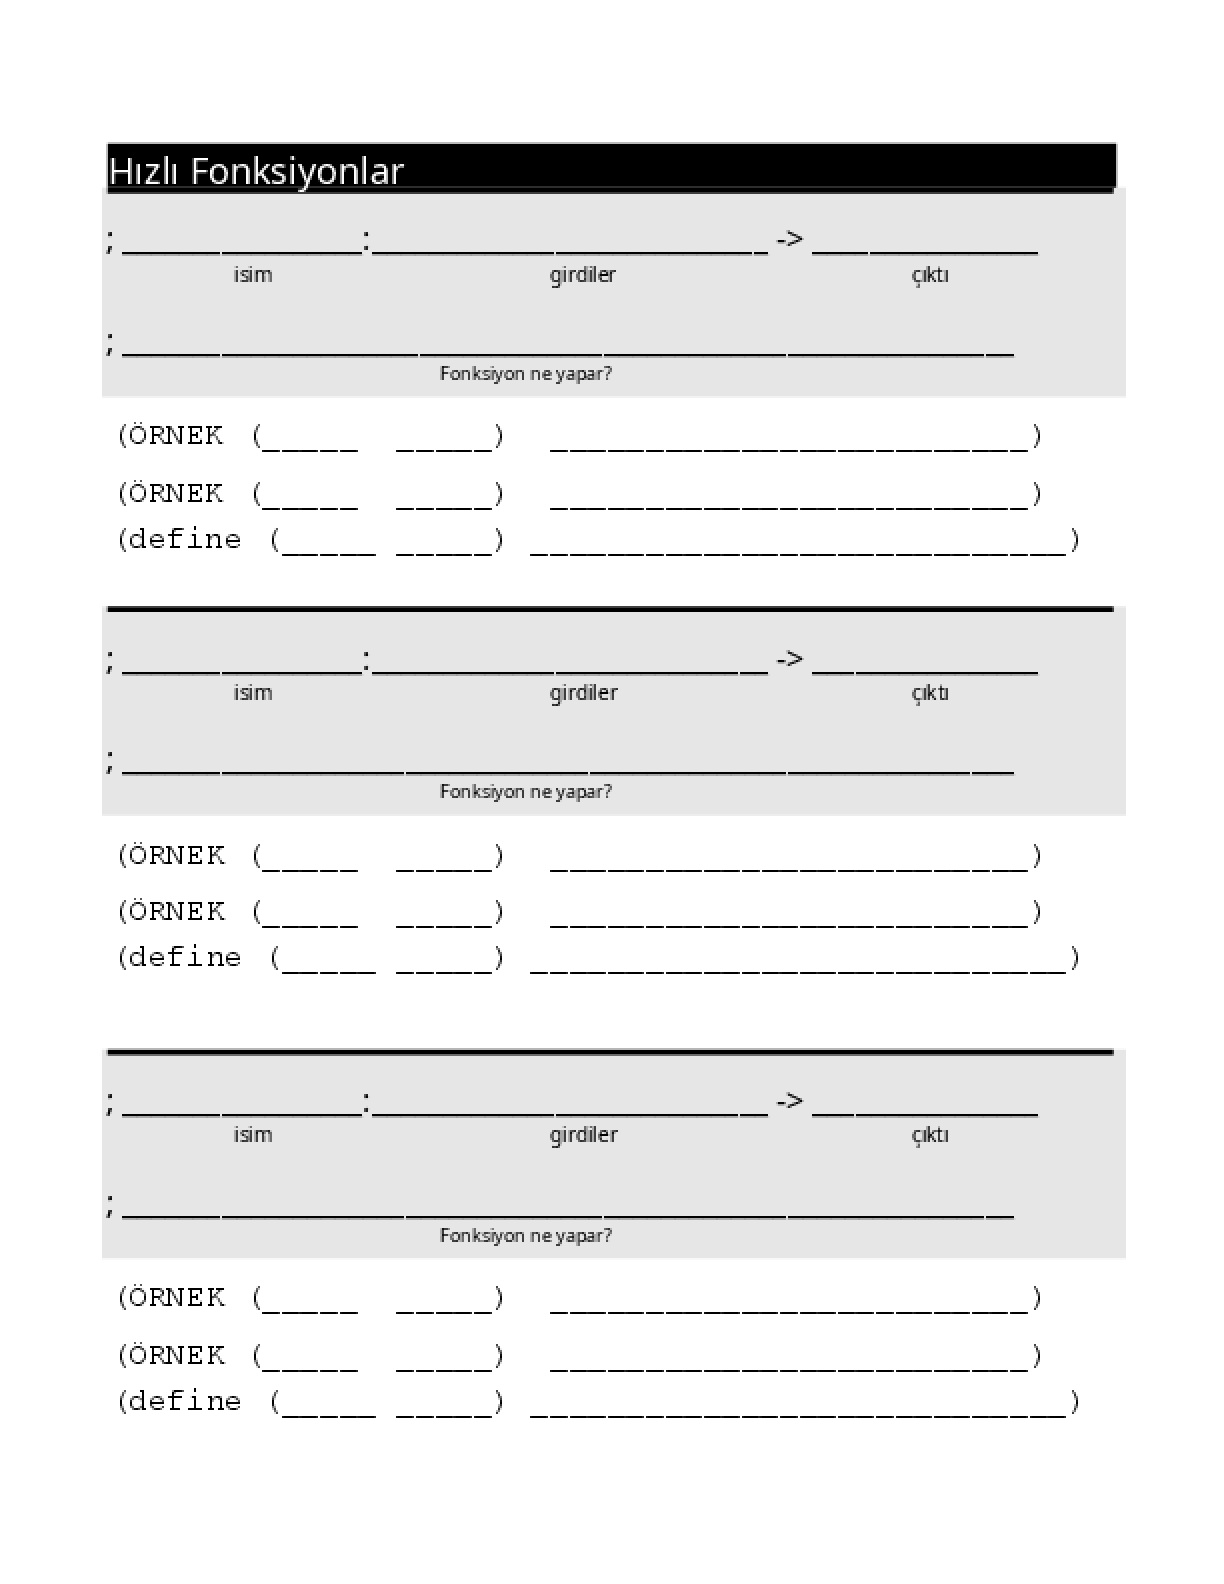
\includegraphics[width=1\linewidth]{cebirsplit-11.png}
\newpage
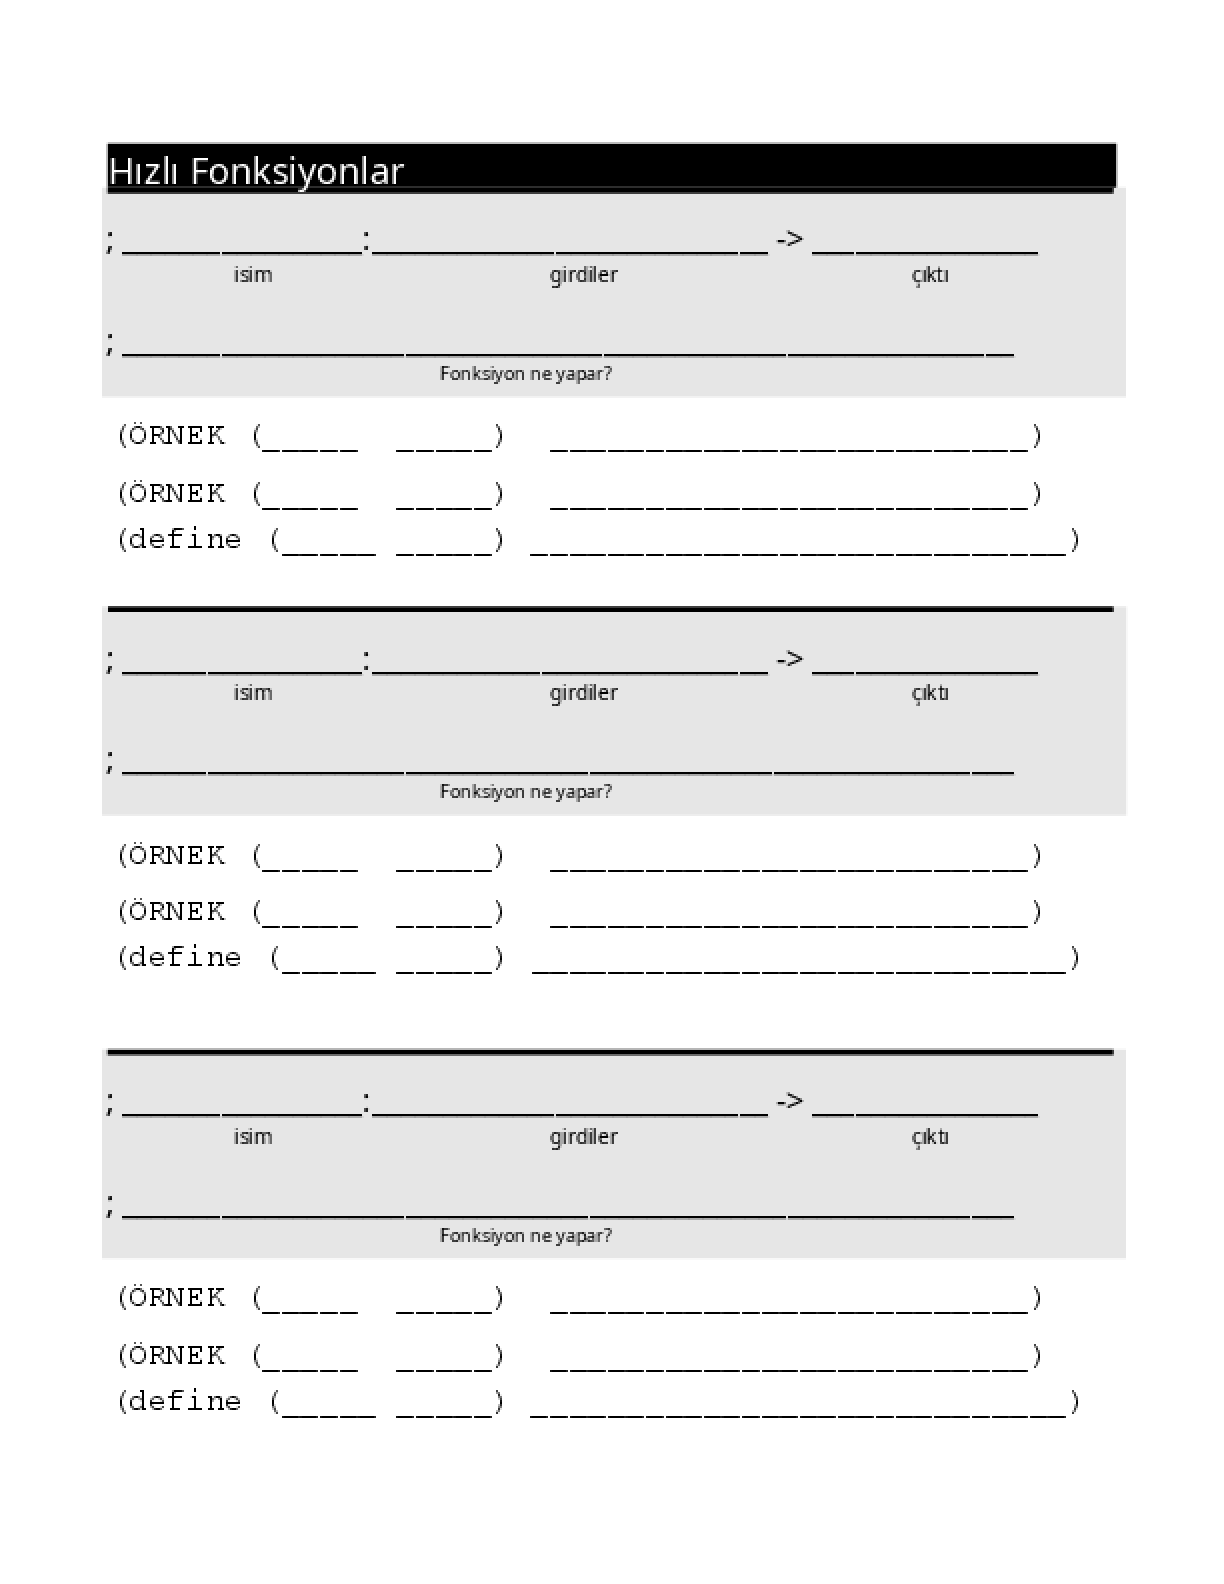
\includegraphics[width=1\linewidth]{cebirsplit-12.png}
\newpage
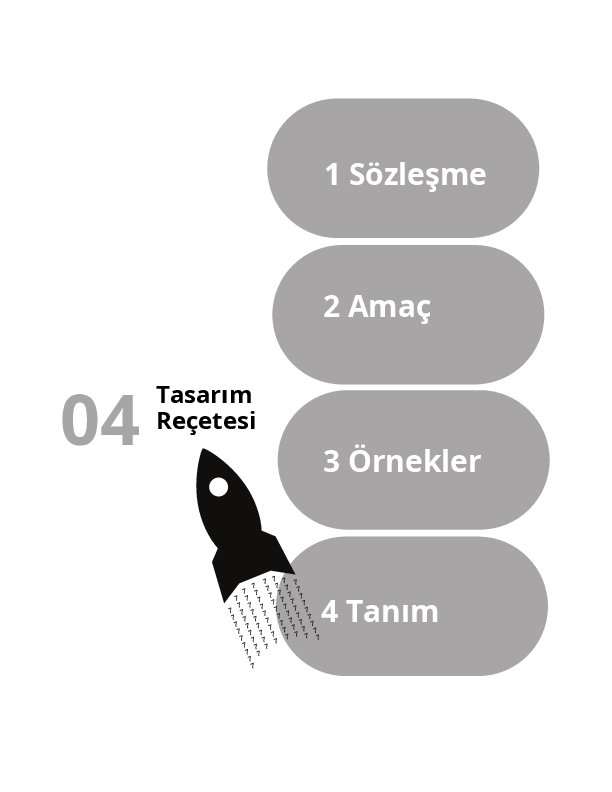
\includegraphics[width=1\linewidth]{cebir-bolum-04-000.png}
\newpage

\noindent \begin{tabular}{p{16cm}}
\section*{Sayfa inşaat sırasında. Orijinalı bir sonraki sayfada}
{\Large \center Problem: Roket Yüksekliği}\\
\textit{Talimatlar: Bir roket saatte 7 m/s hızla hareket edecek şekilde havalanıyor. Roketin kalktığı andan itibaren geçen süreyi alan ve roketin yüksekliğini veren, roket-yüksekliği adında bir fonksiyon yazınız.}\\
\large Sözleşme ve Amaç Açıklaması\\
\textit{Her sözleşme üç bölümden oluşur...}\\
% \\
\end{tabular}\\
\noindent \begin{tabular}{L{4cm} L{6cm} L{6cm}}
;\dotfill &:\dotfill &$\rightarrow$\dotfill \\
\end{tabular}
\noindent \begin{tabular}{C{4cm} C{6cm} C{6cm}}
\textit{fonksiyon adı} & \textit{girdiler} & \textit{çıktı} \\
\end{tabular}\\
\\
\noindent \begin{tabular}{L{17cm}}
{;\dotfill}\\
\end{tabular}
\noindent \begin{tabular}{C{17cm}}
{\textit{Fonksiyon ne yapar?}}\\
\end{tabular}

%Örnekler
%Birkaç örnek yazıp, değişenleri yuvarlak içine alarak işaretleyiniz.
%(ÖRNEK())
%fonksiyon adı&girdi(ler)&Fonksiyonun ürettiği nedir?
%Tanım
%Tanımı ve her değişken için verilen isimleri yazınız.
%(define ()
%fonksiyon adı&Değişkenler ya da girdiler
%Fonksiyon verilen değişkenlerle ne yapar? 
\newpage
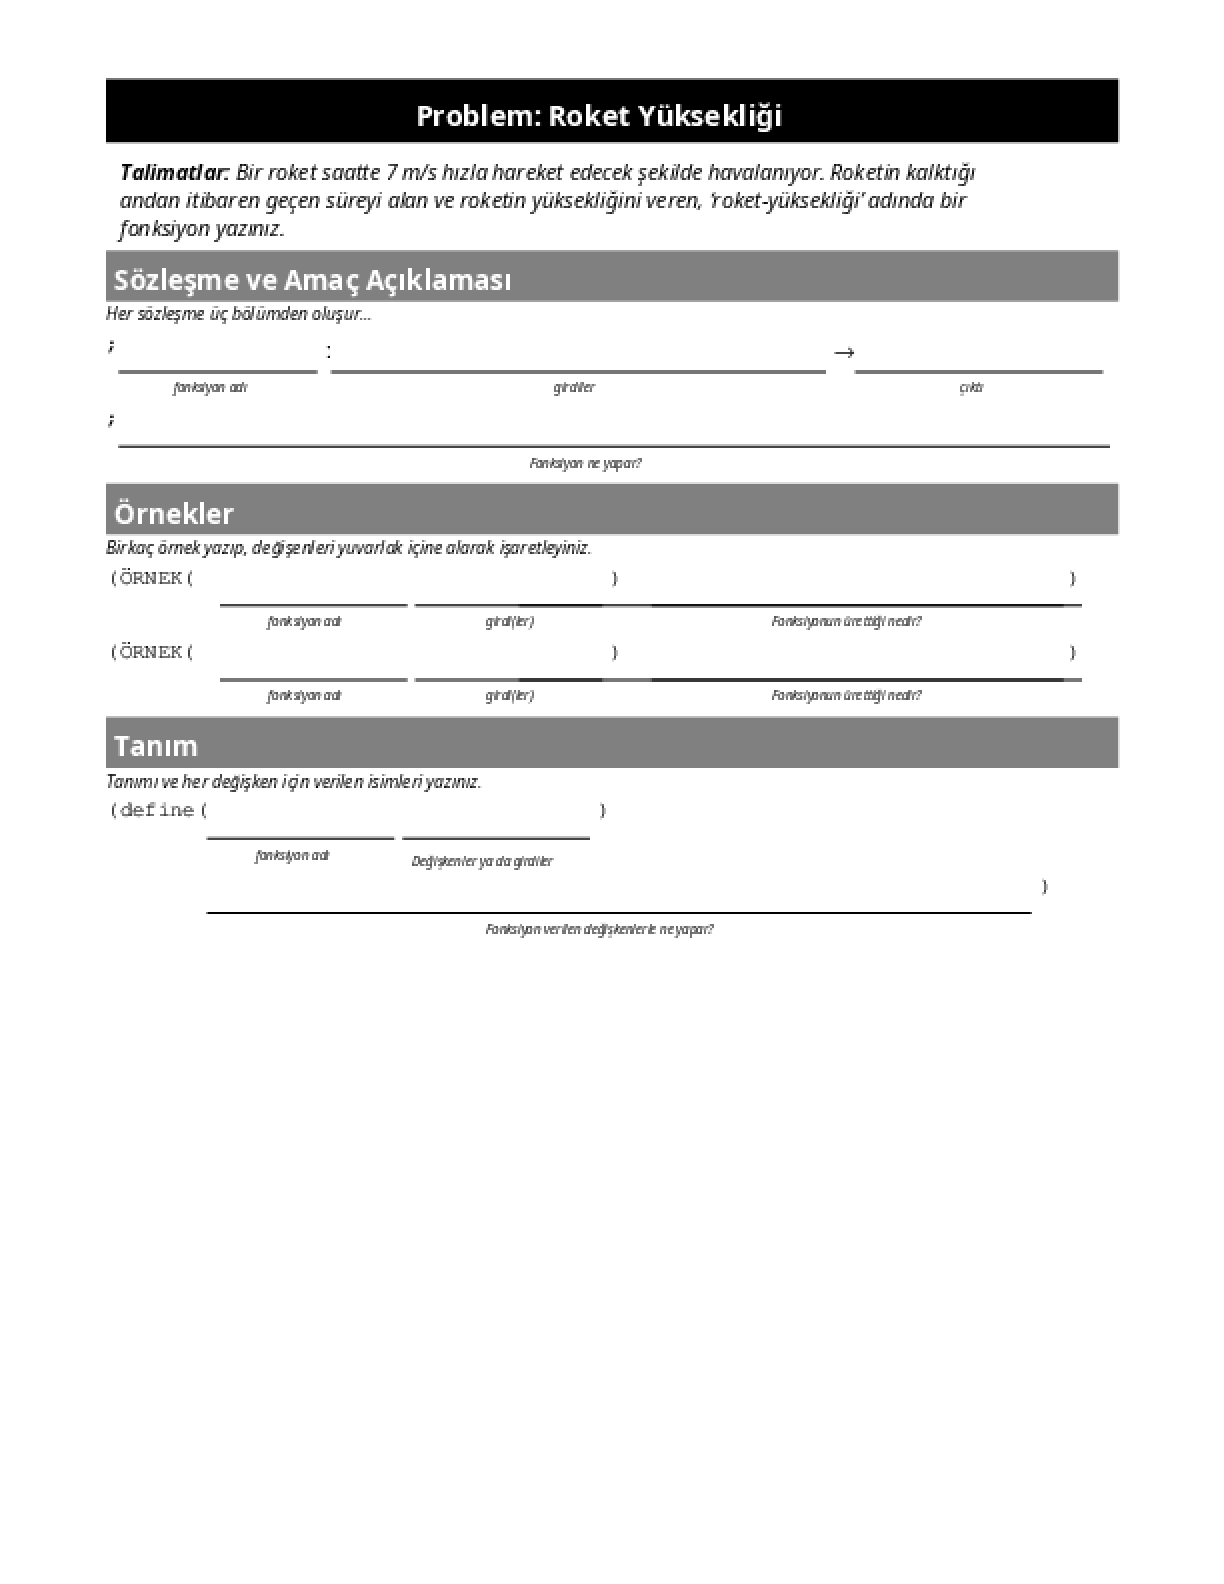
\includegraphics[width=1\linewidth]{cebirsplit-14.png}
\newpage
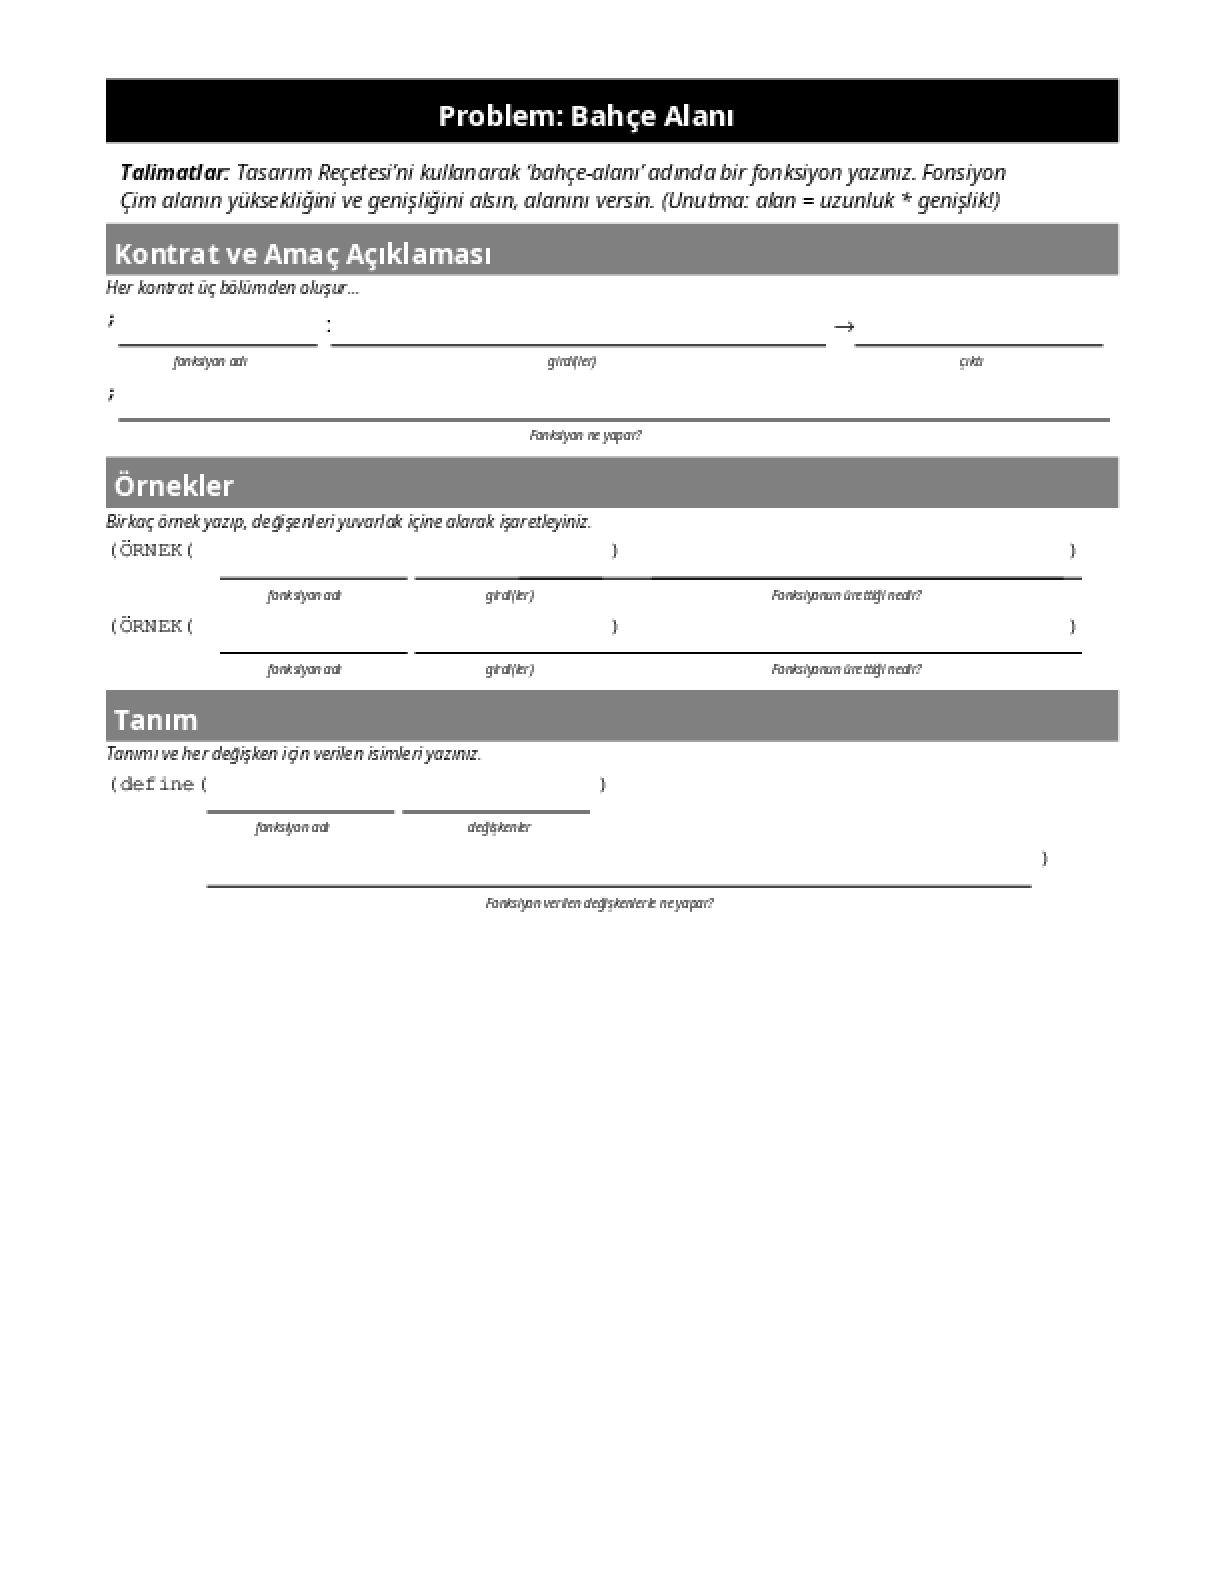
\includegraphics[width=1\linewidth]{cebirsplit-15.png}
\newpage
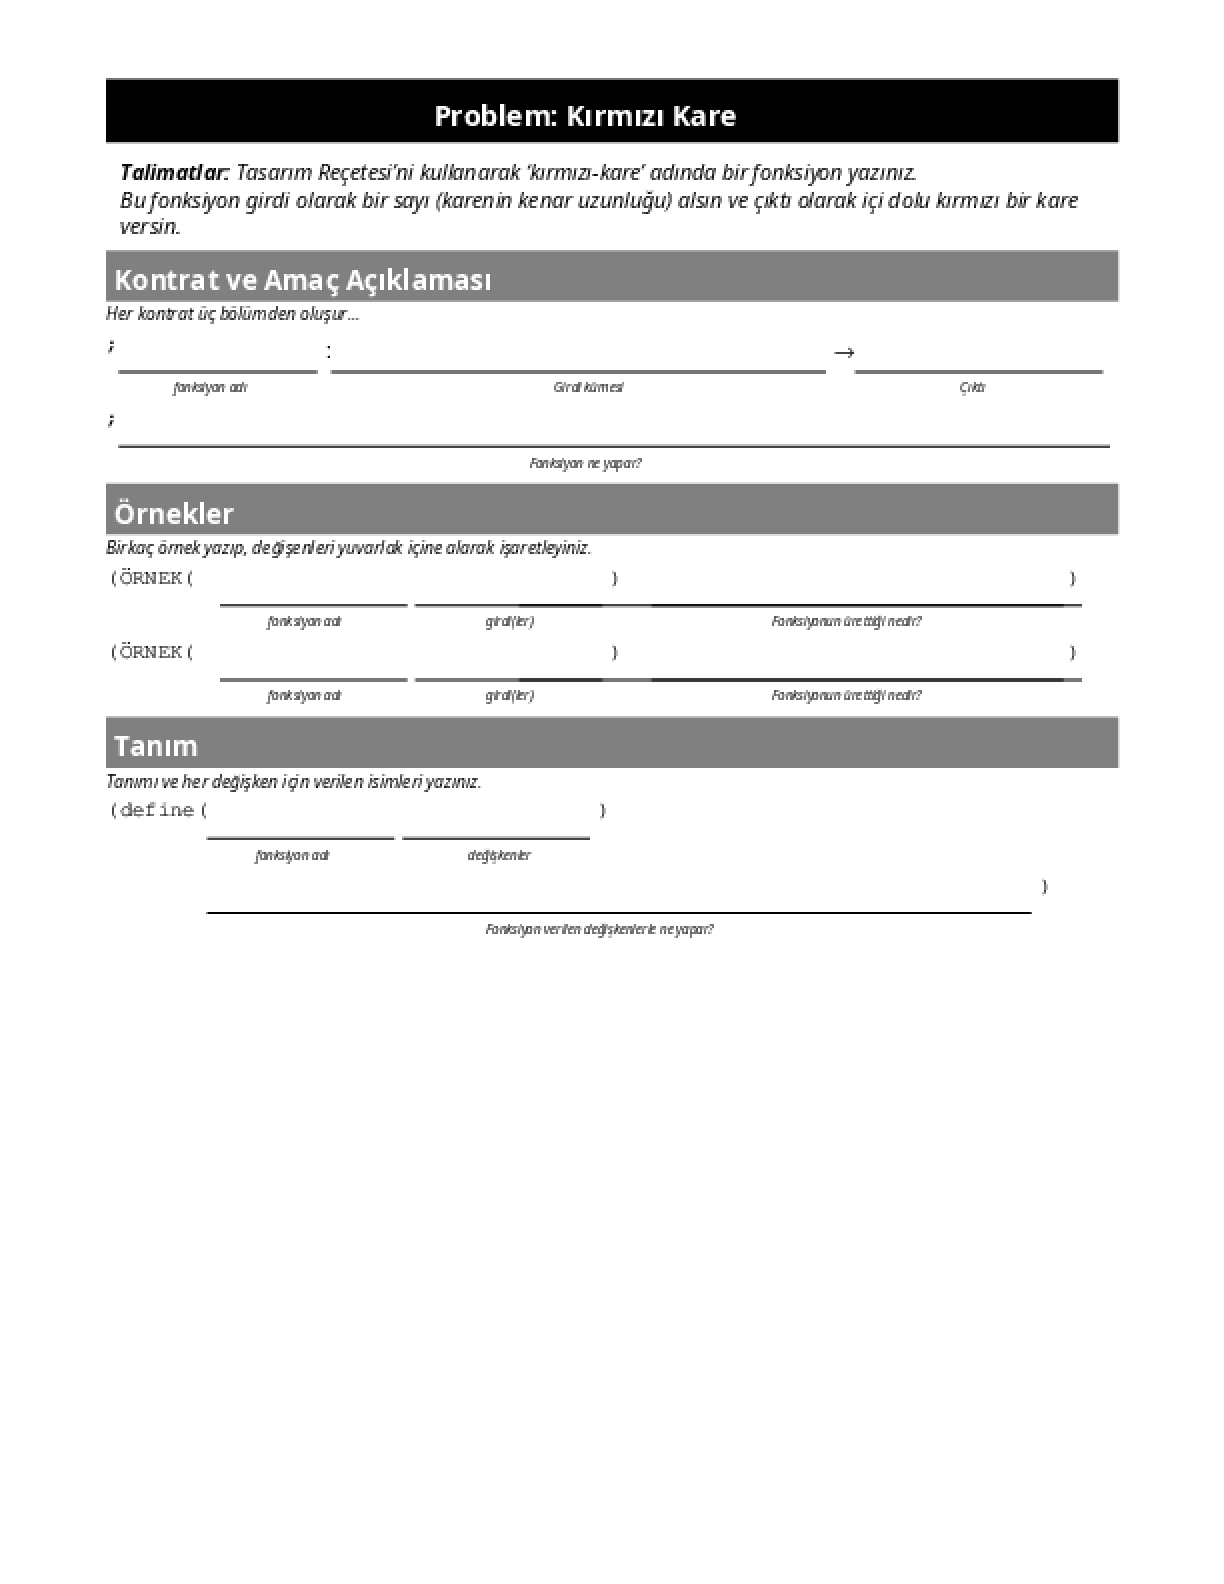
\includegraphics[width=1\linewidth]{cebirsplit-16.png}
\newpage
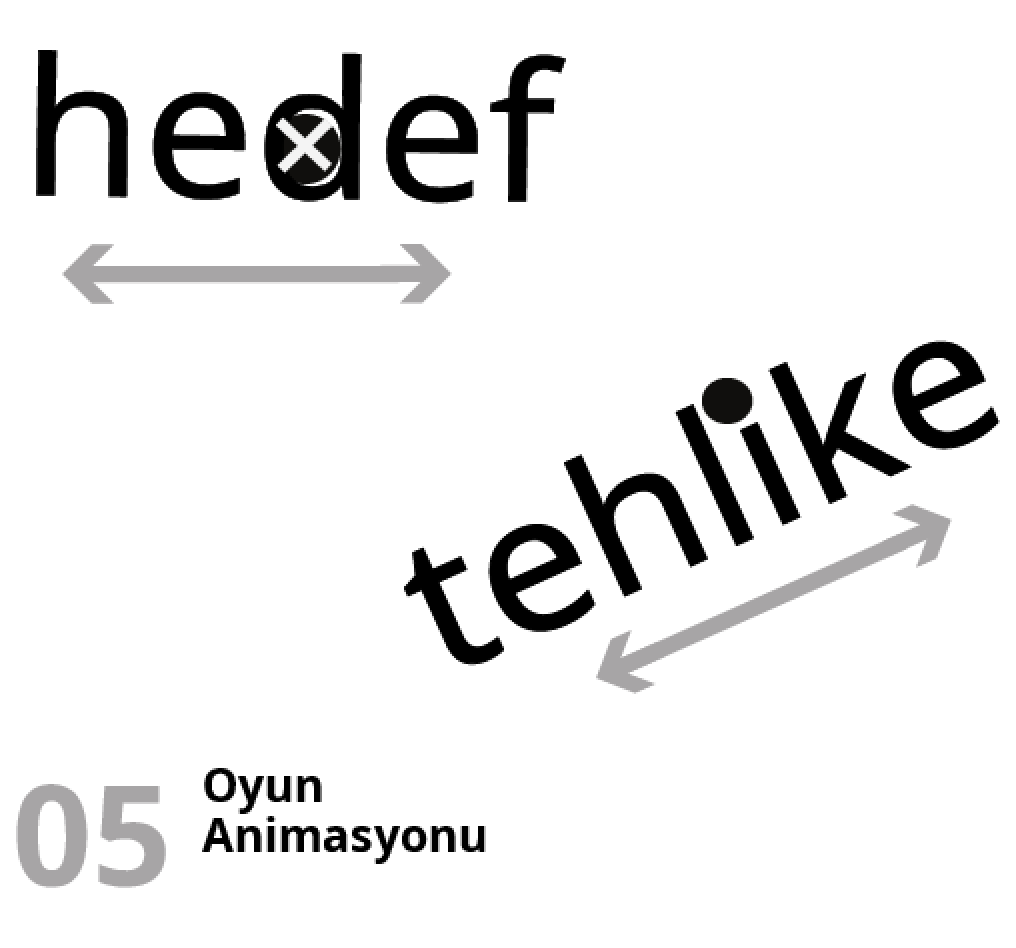
\includegraphics[width=1\linewidth]{cebir-bolum-05-000.png}
\newpage
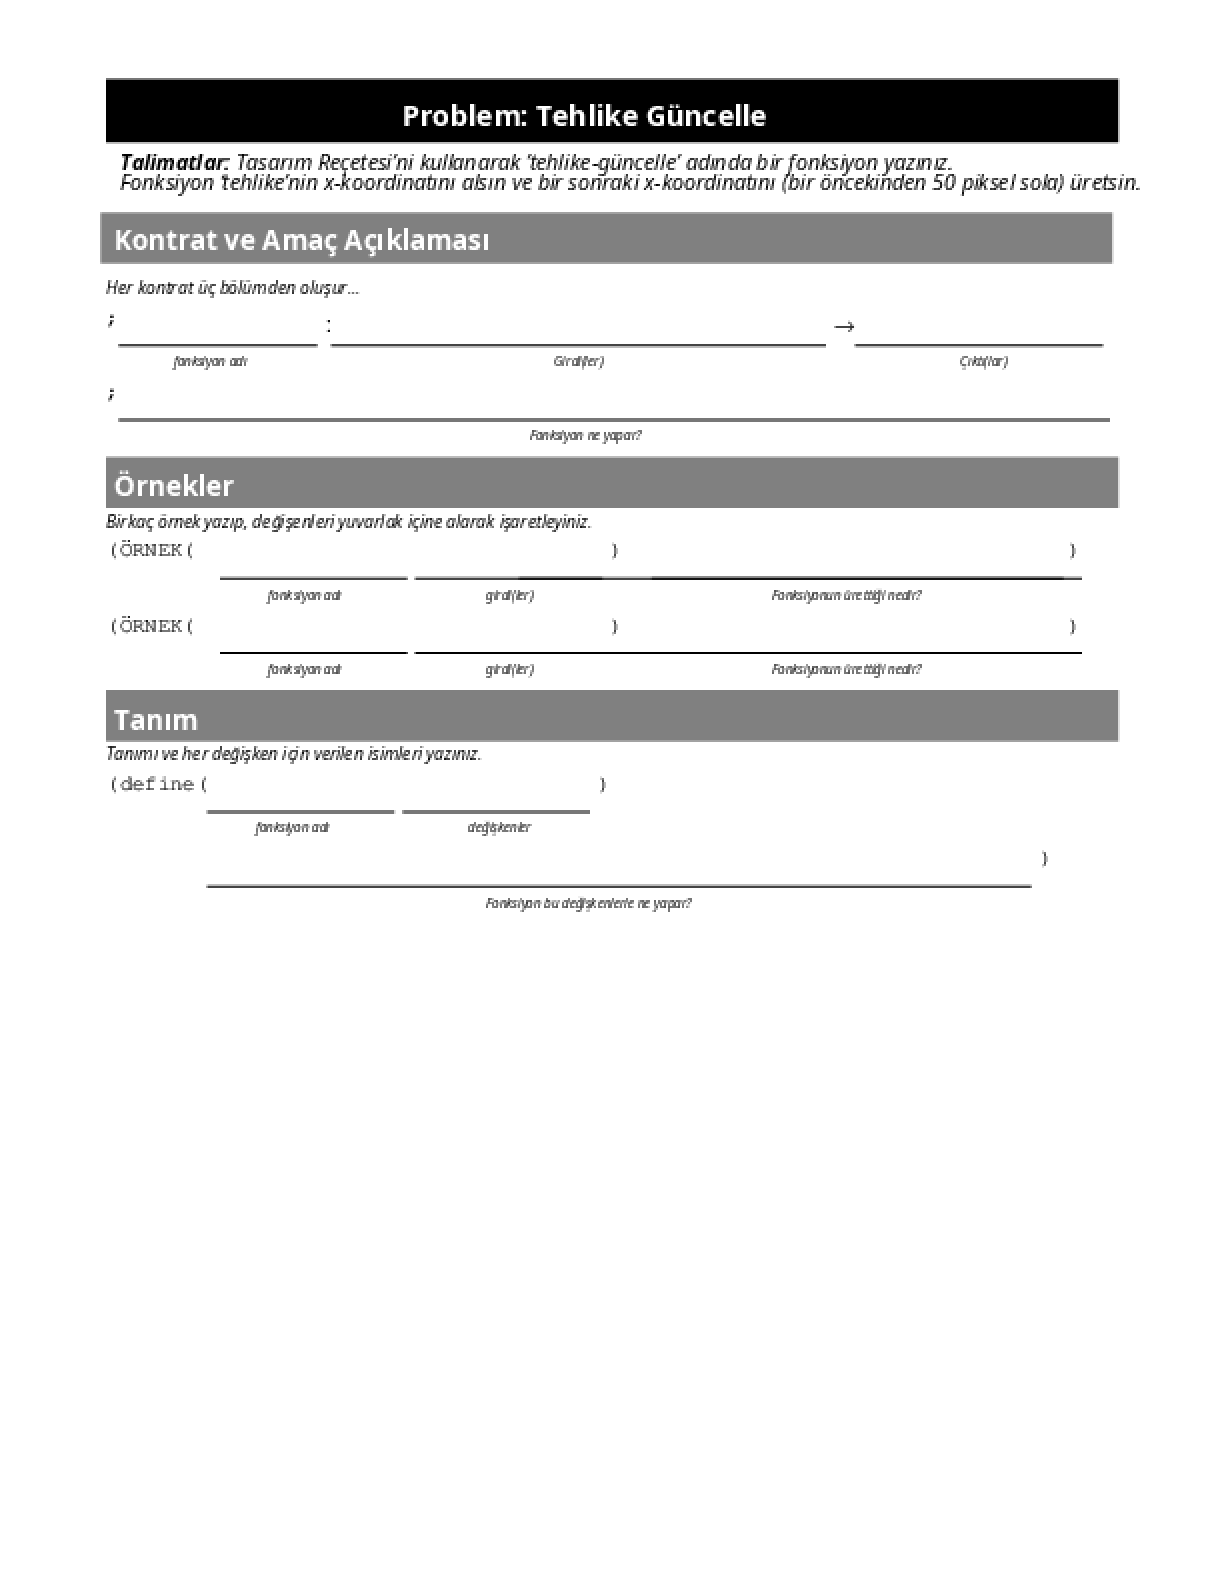
\includegraphics[width=1\linewidth]{cebirsplit-18.png}
\newpage
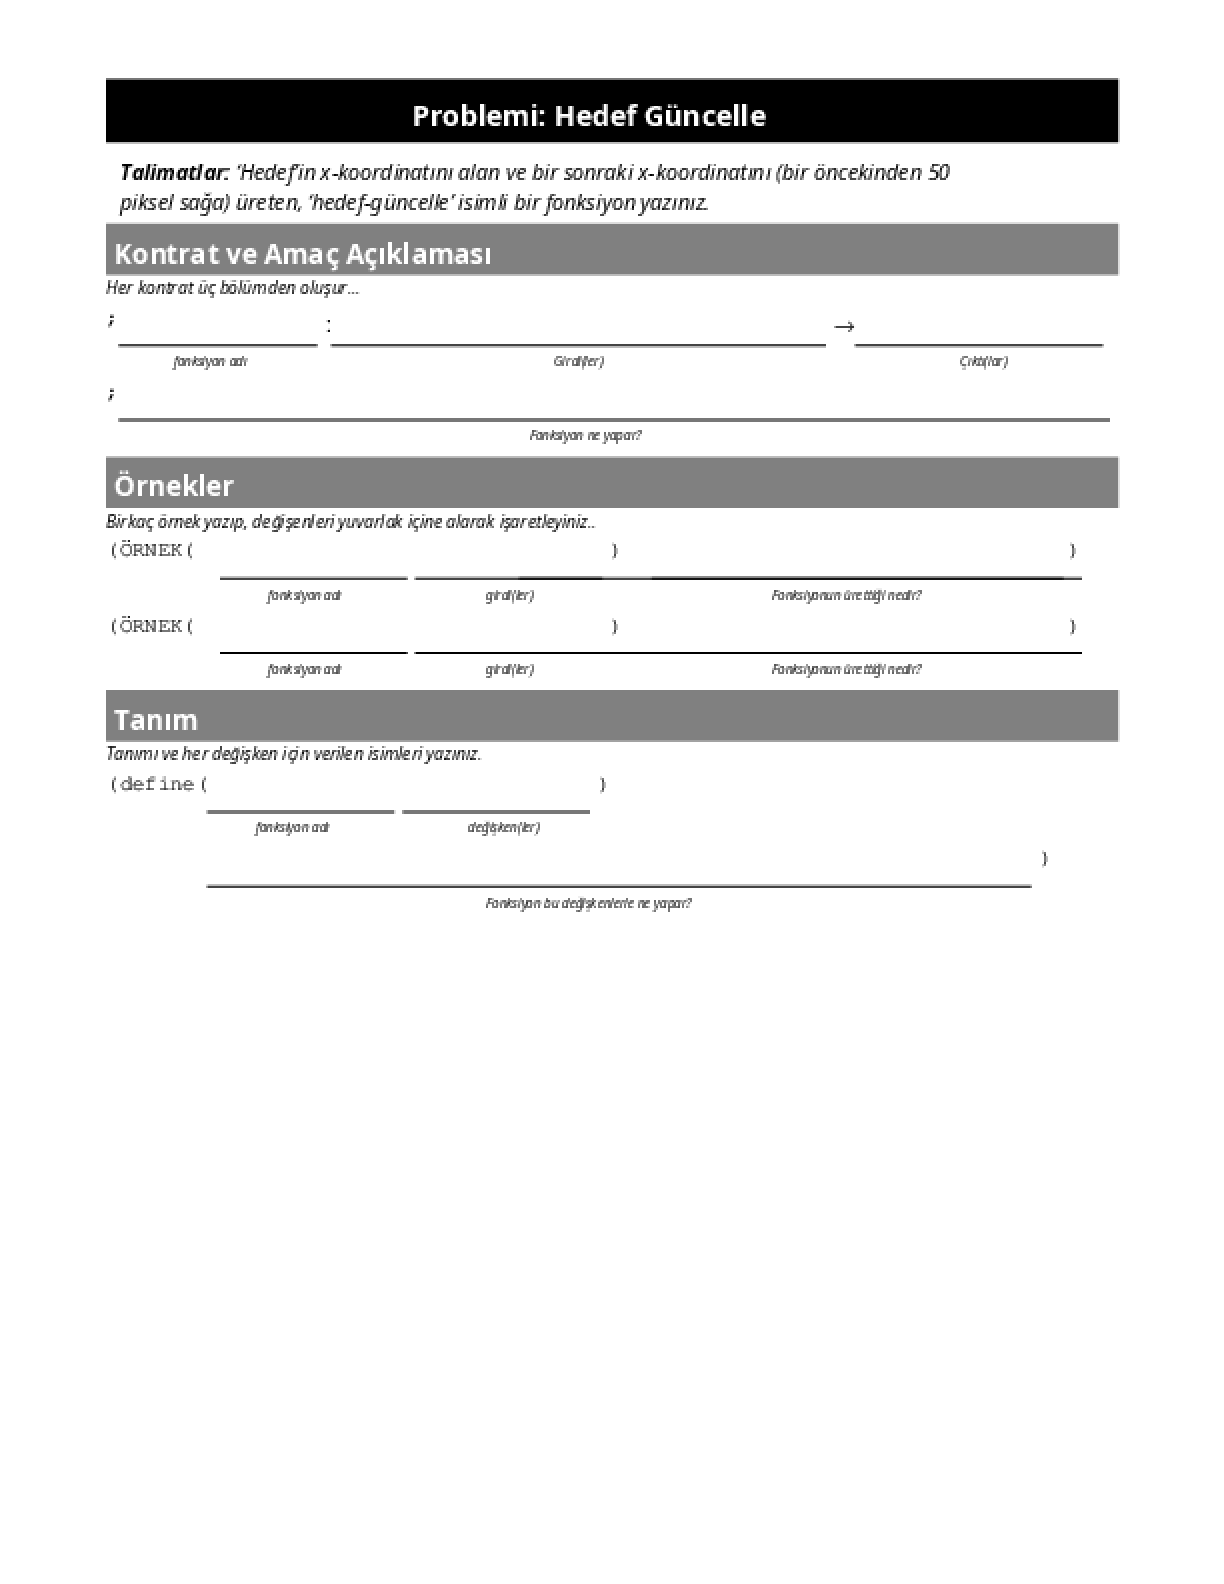
\includegraphics[width=1\linewidth]{cebirsplit-19.png}
\newpage
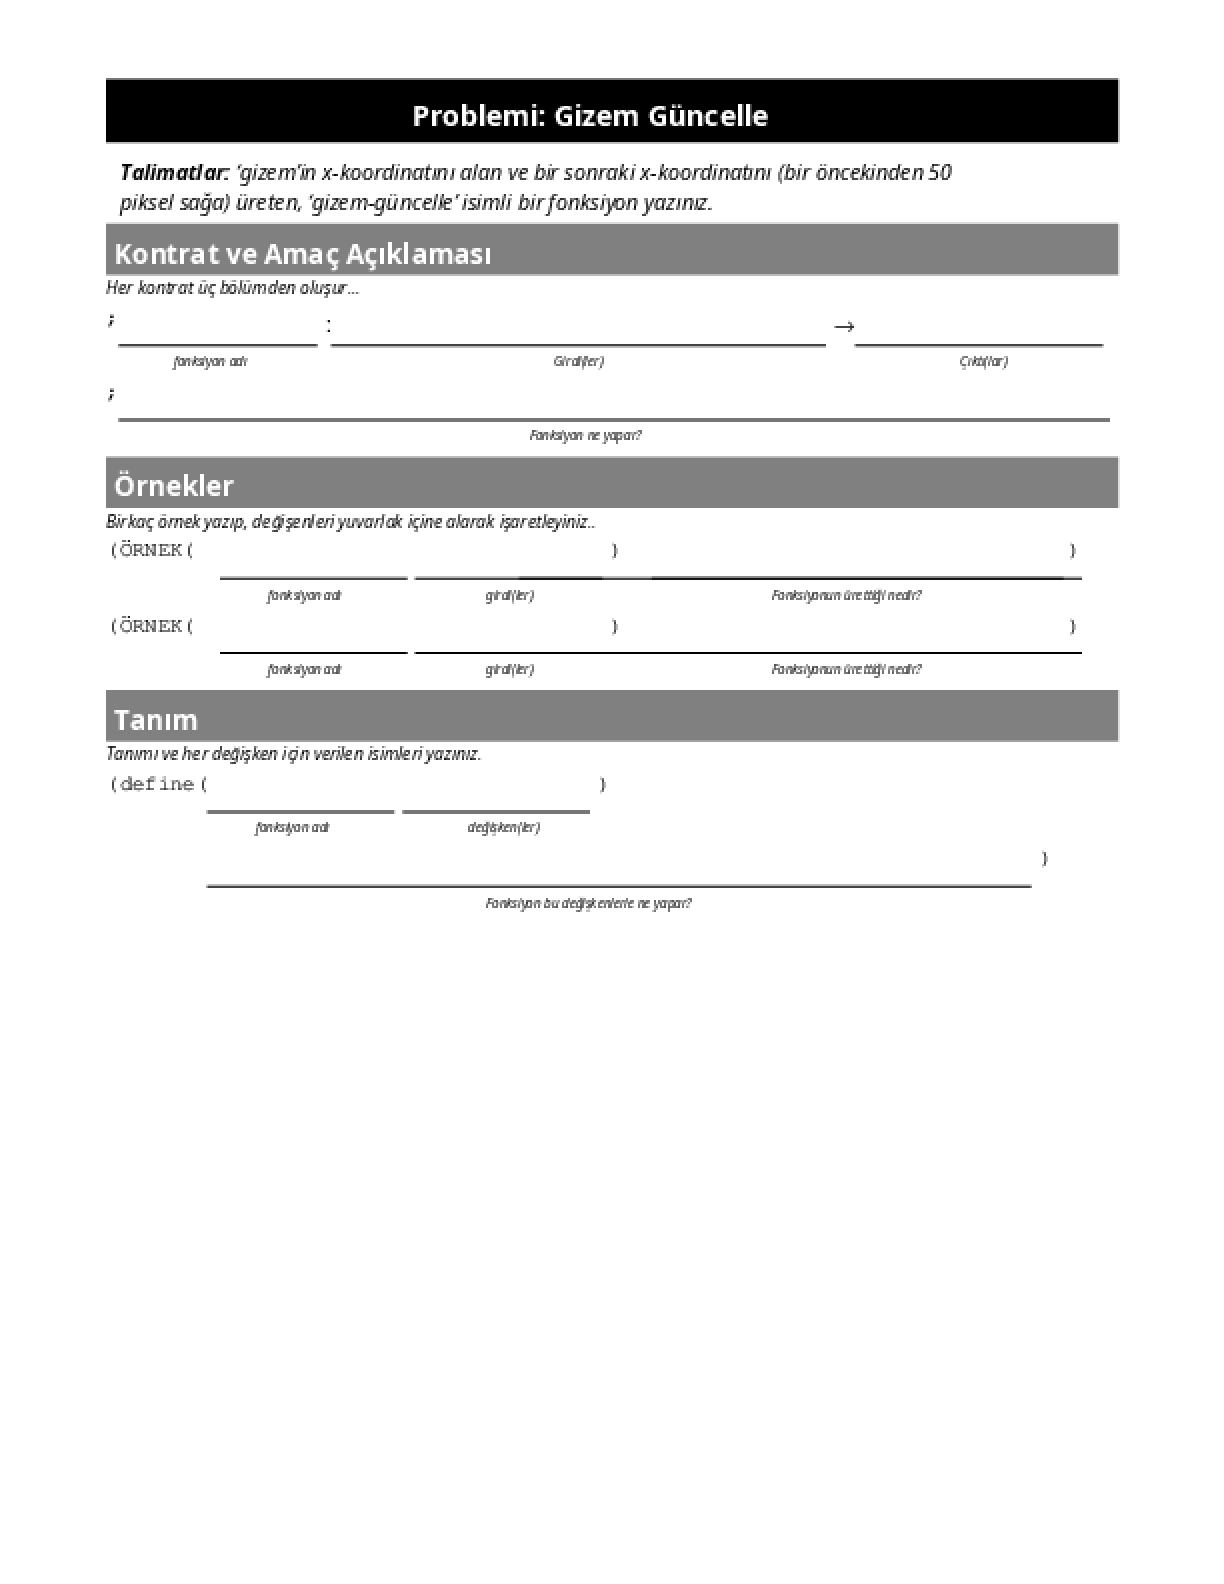
\includegraphics[width=1\linewidth]{cebirsplit-20.png}
\newpage
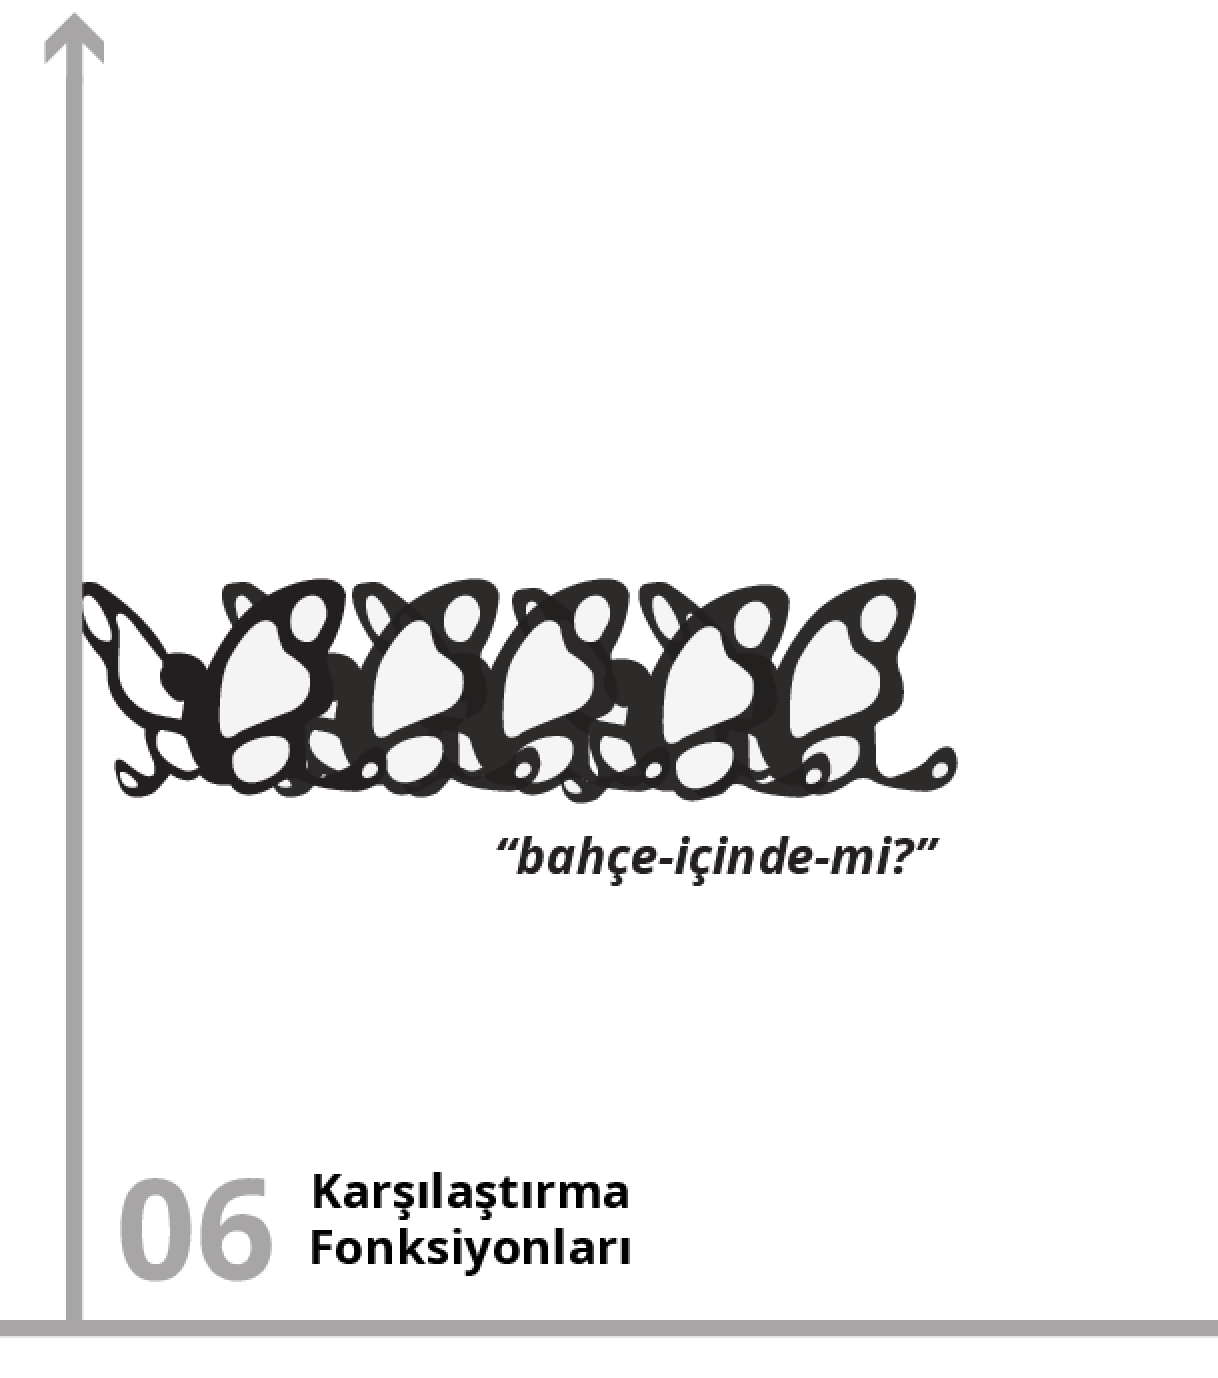
\includegraphics[width=1.2\linewidth]{cebir-bolum-06-000.png}
\newpage
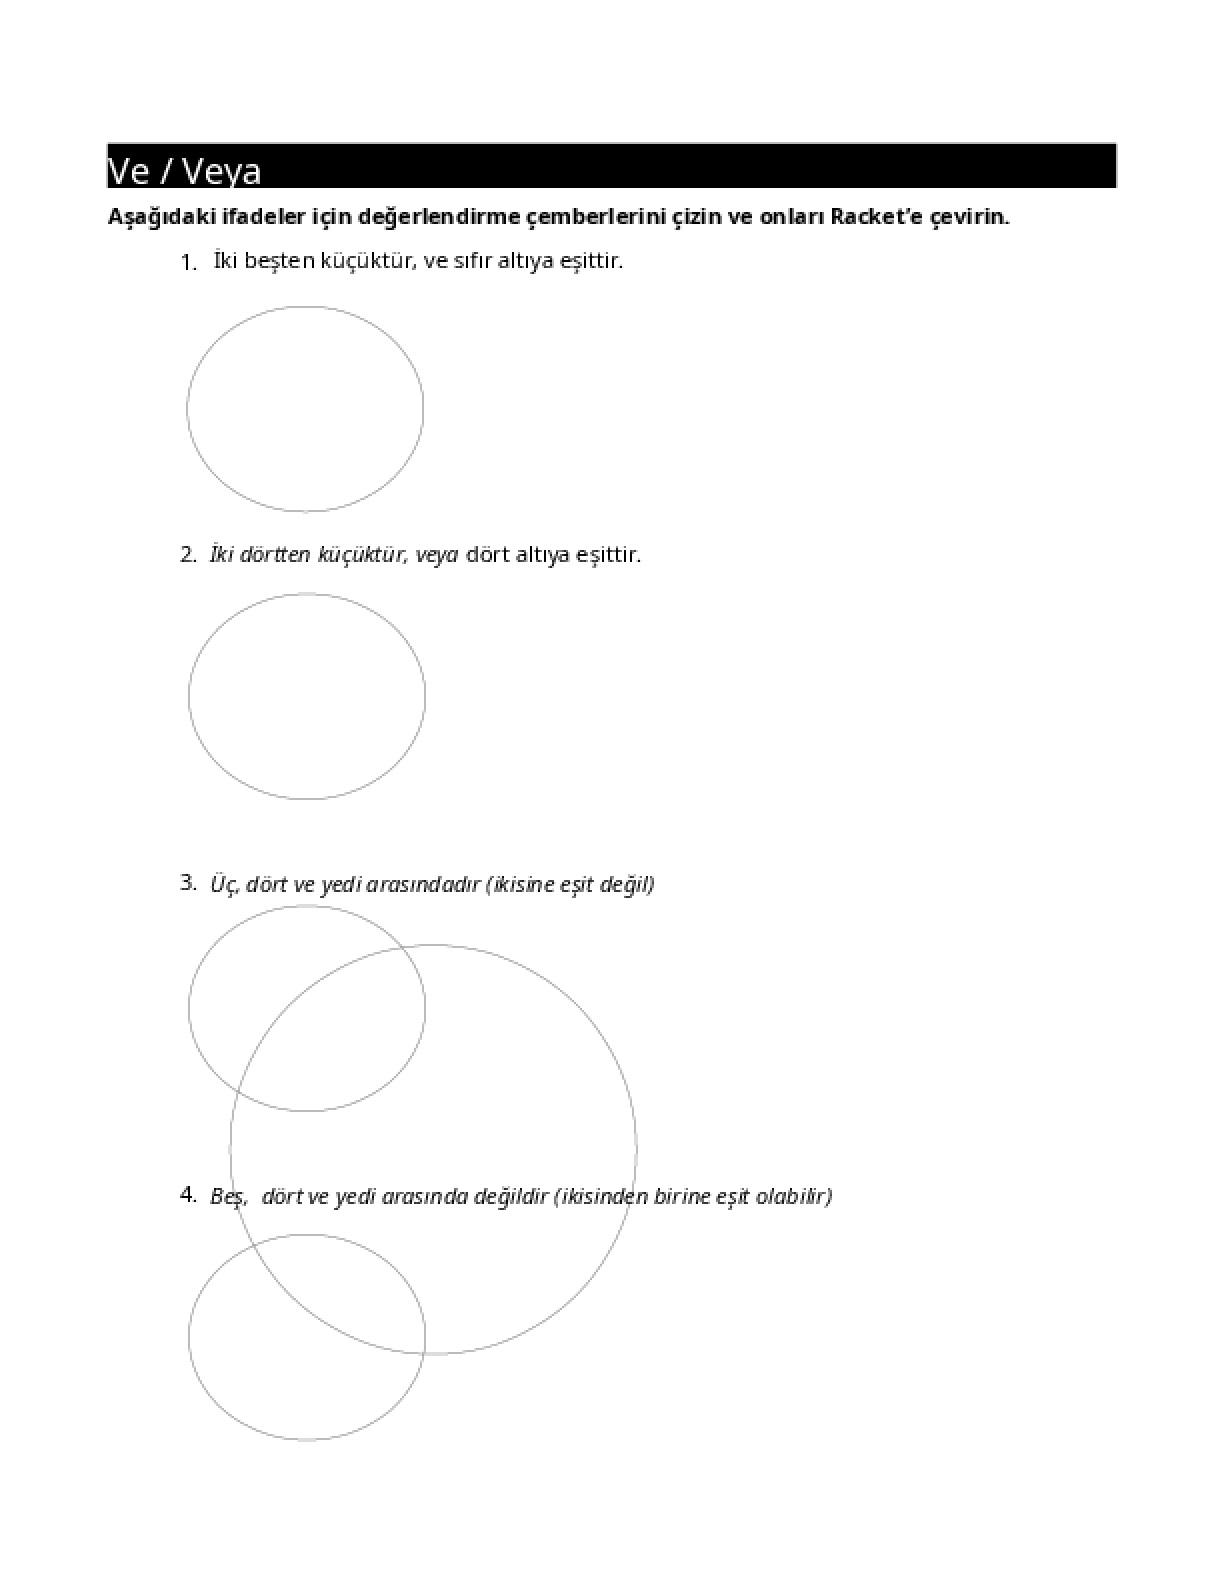
\includegraphics[width=1\linewidth]{cebirsplit-22.png}
\newpage
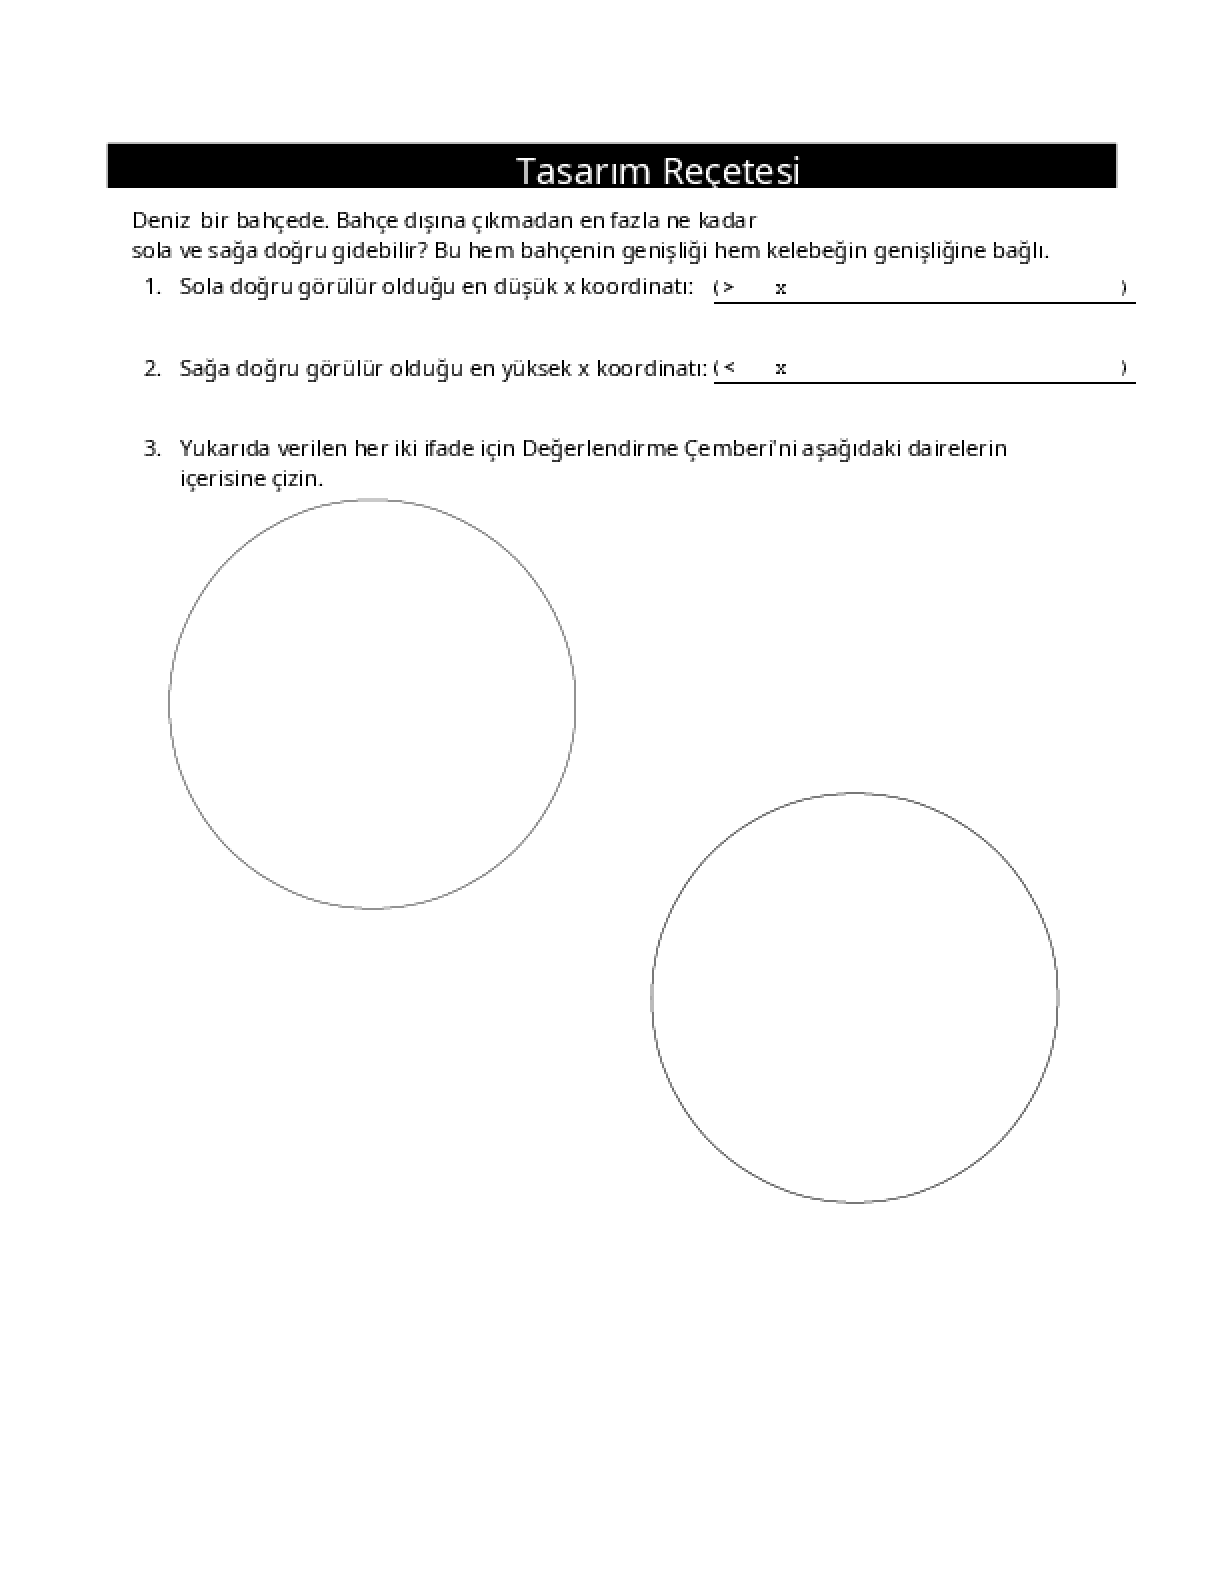
\includegraphics[width=1\linewidth]{cebirsplit-23.png}
\newpage
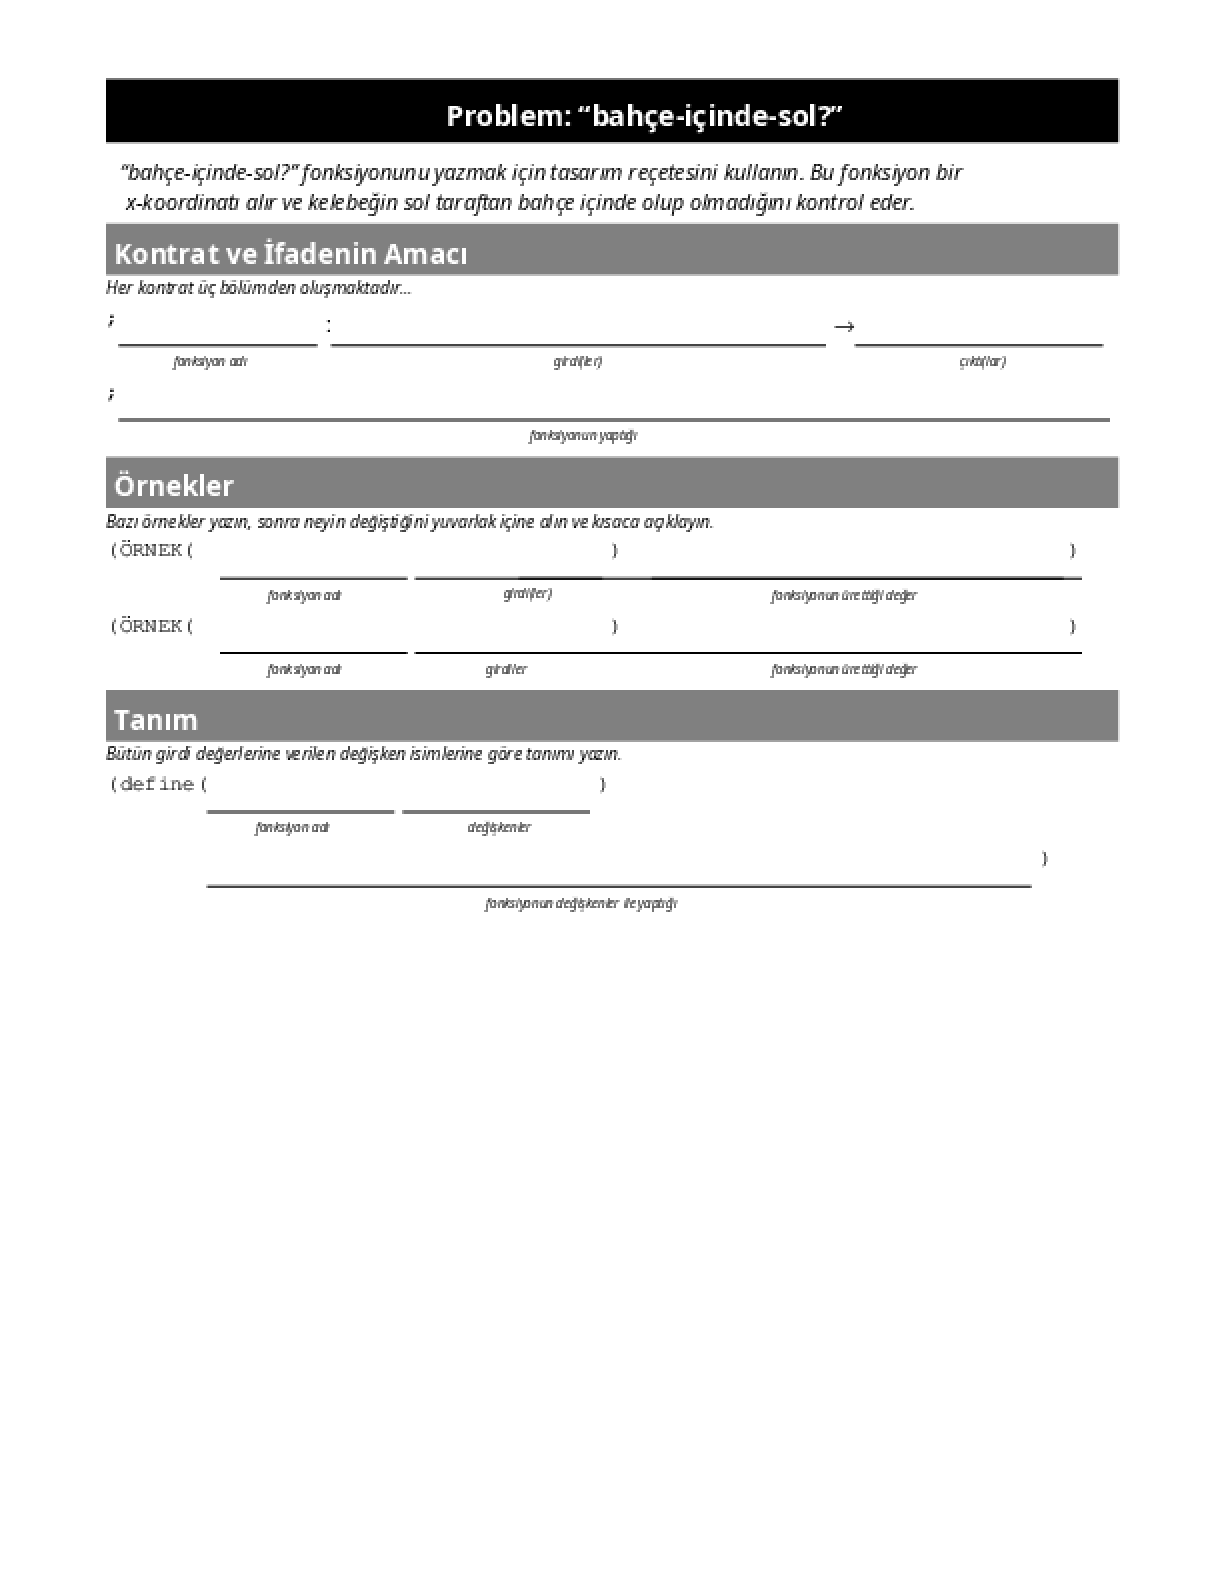
\includegraphics[width=1\linewidth]{cebirsplit-24.png}
\newpage
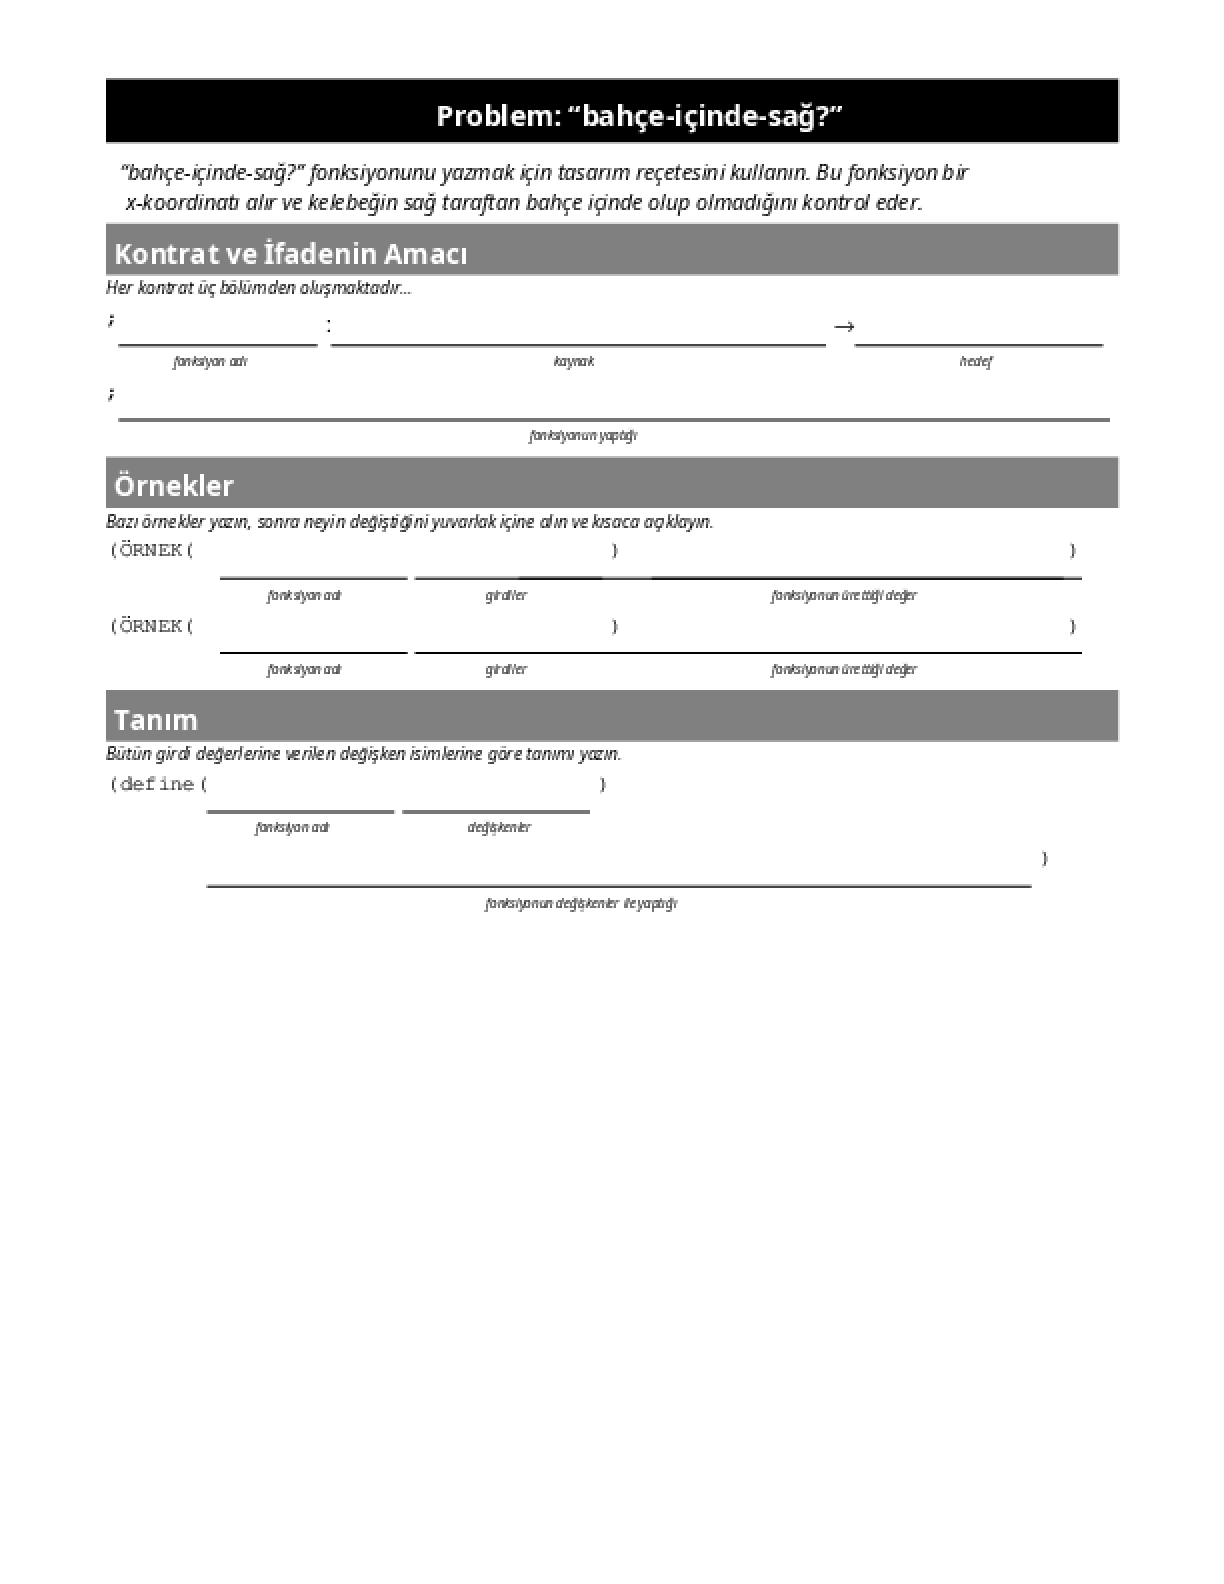
\includegraphics[width=1\linewidth]{cebirsplit-25.png}
\newpage
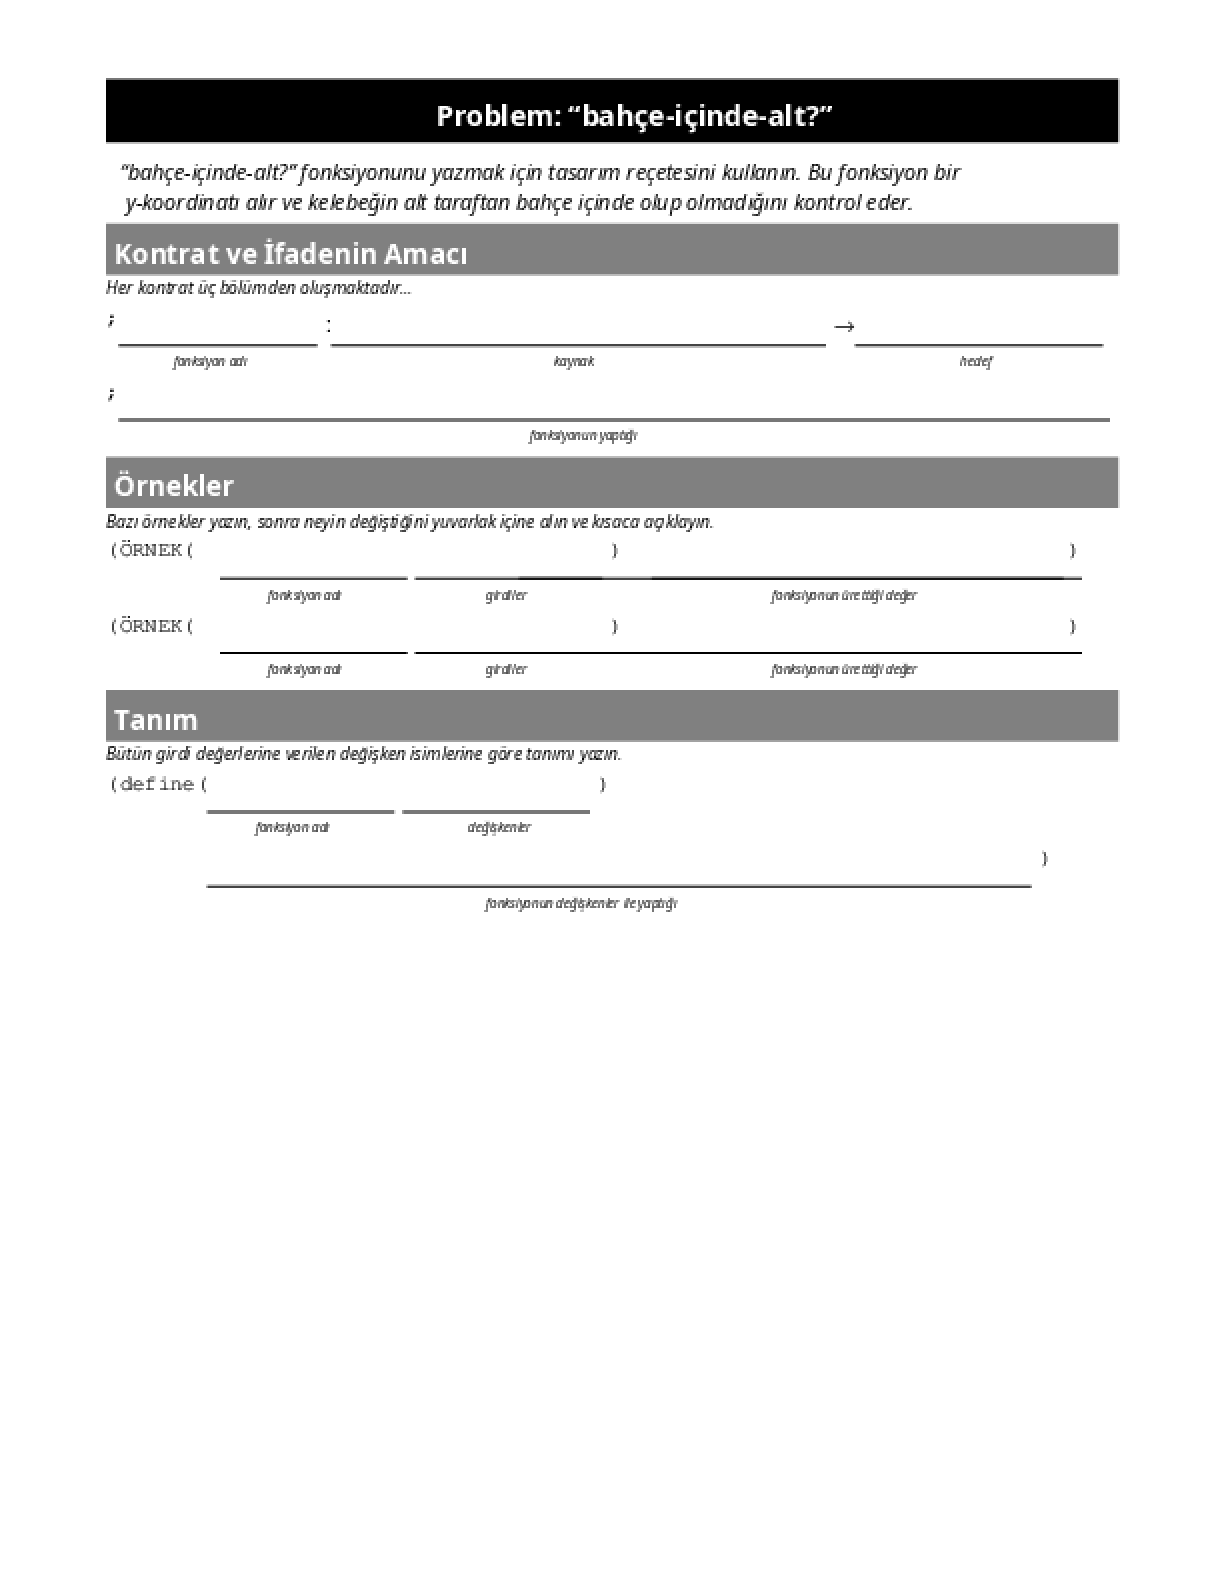
\includegraphics[width=1\linewidth]{cebirsplit-26.png}
\newpage
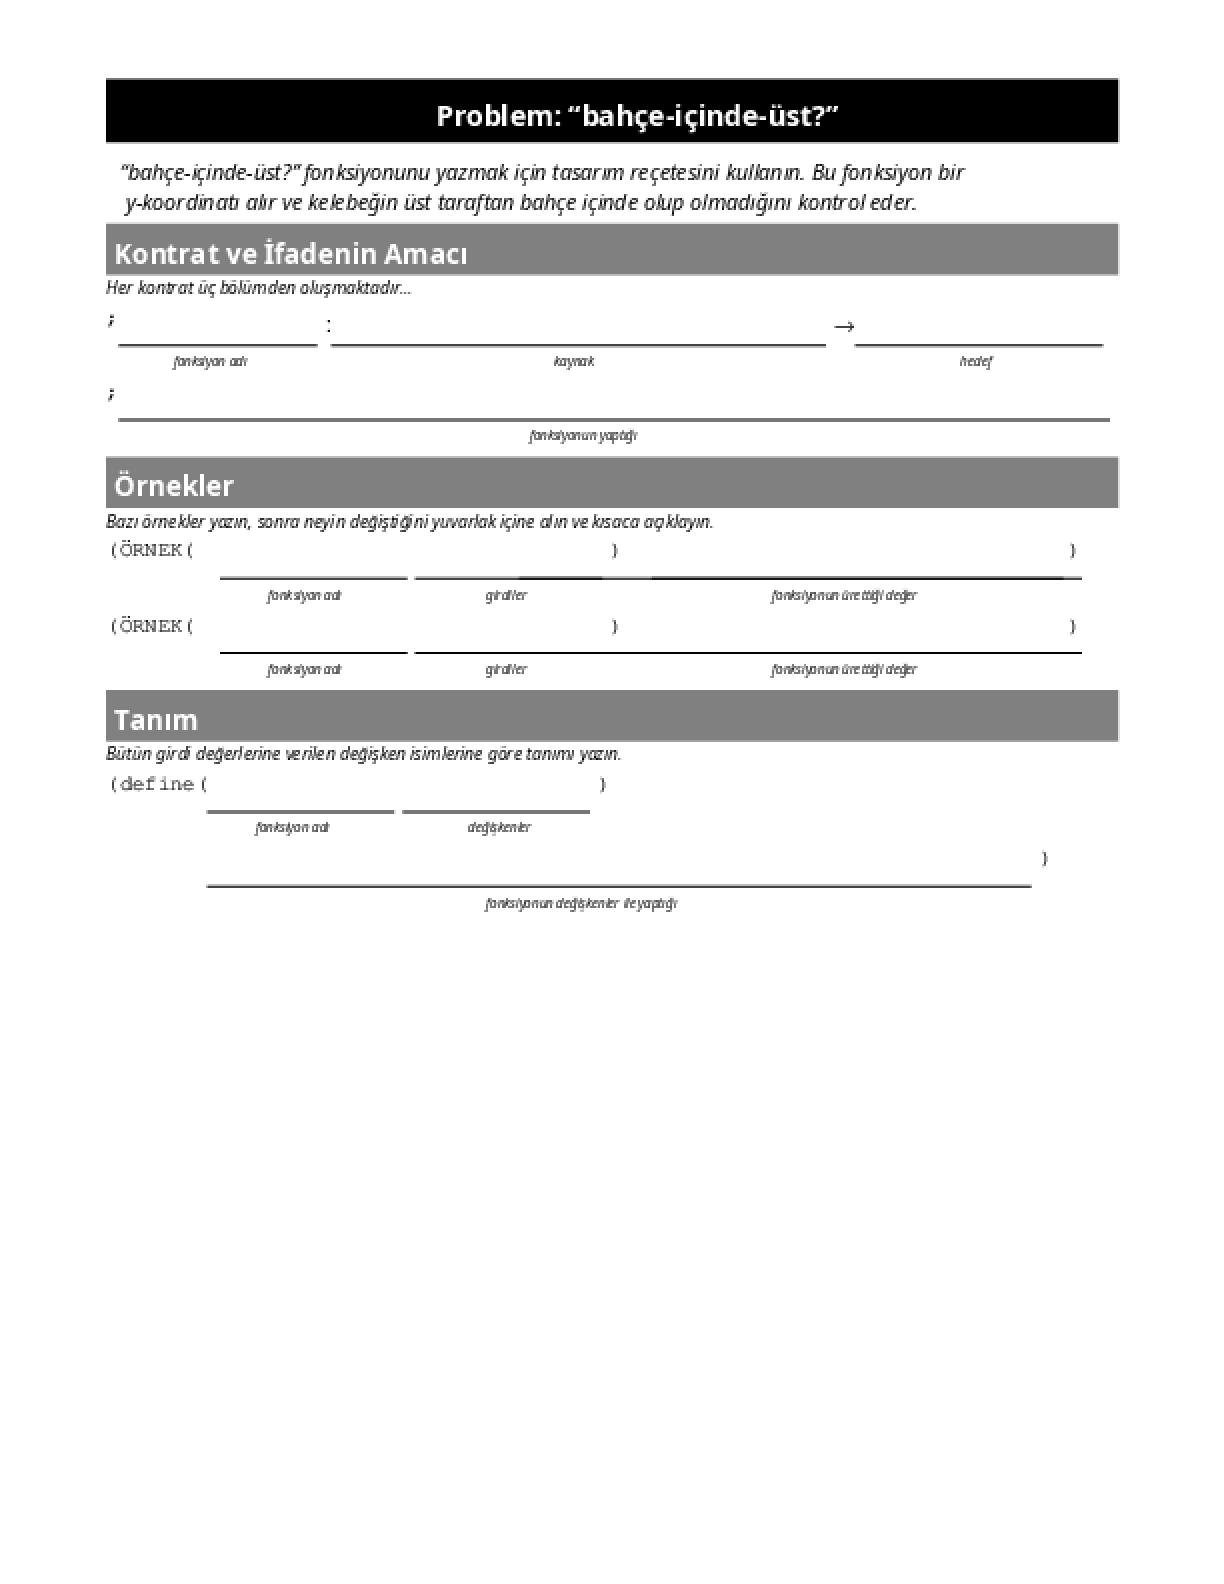
\includegraphics[width=1\linewidth]{cebirsplit-27.png}
\newpage
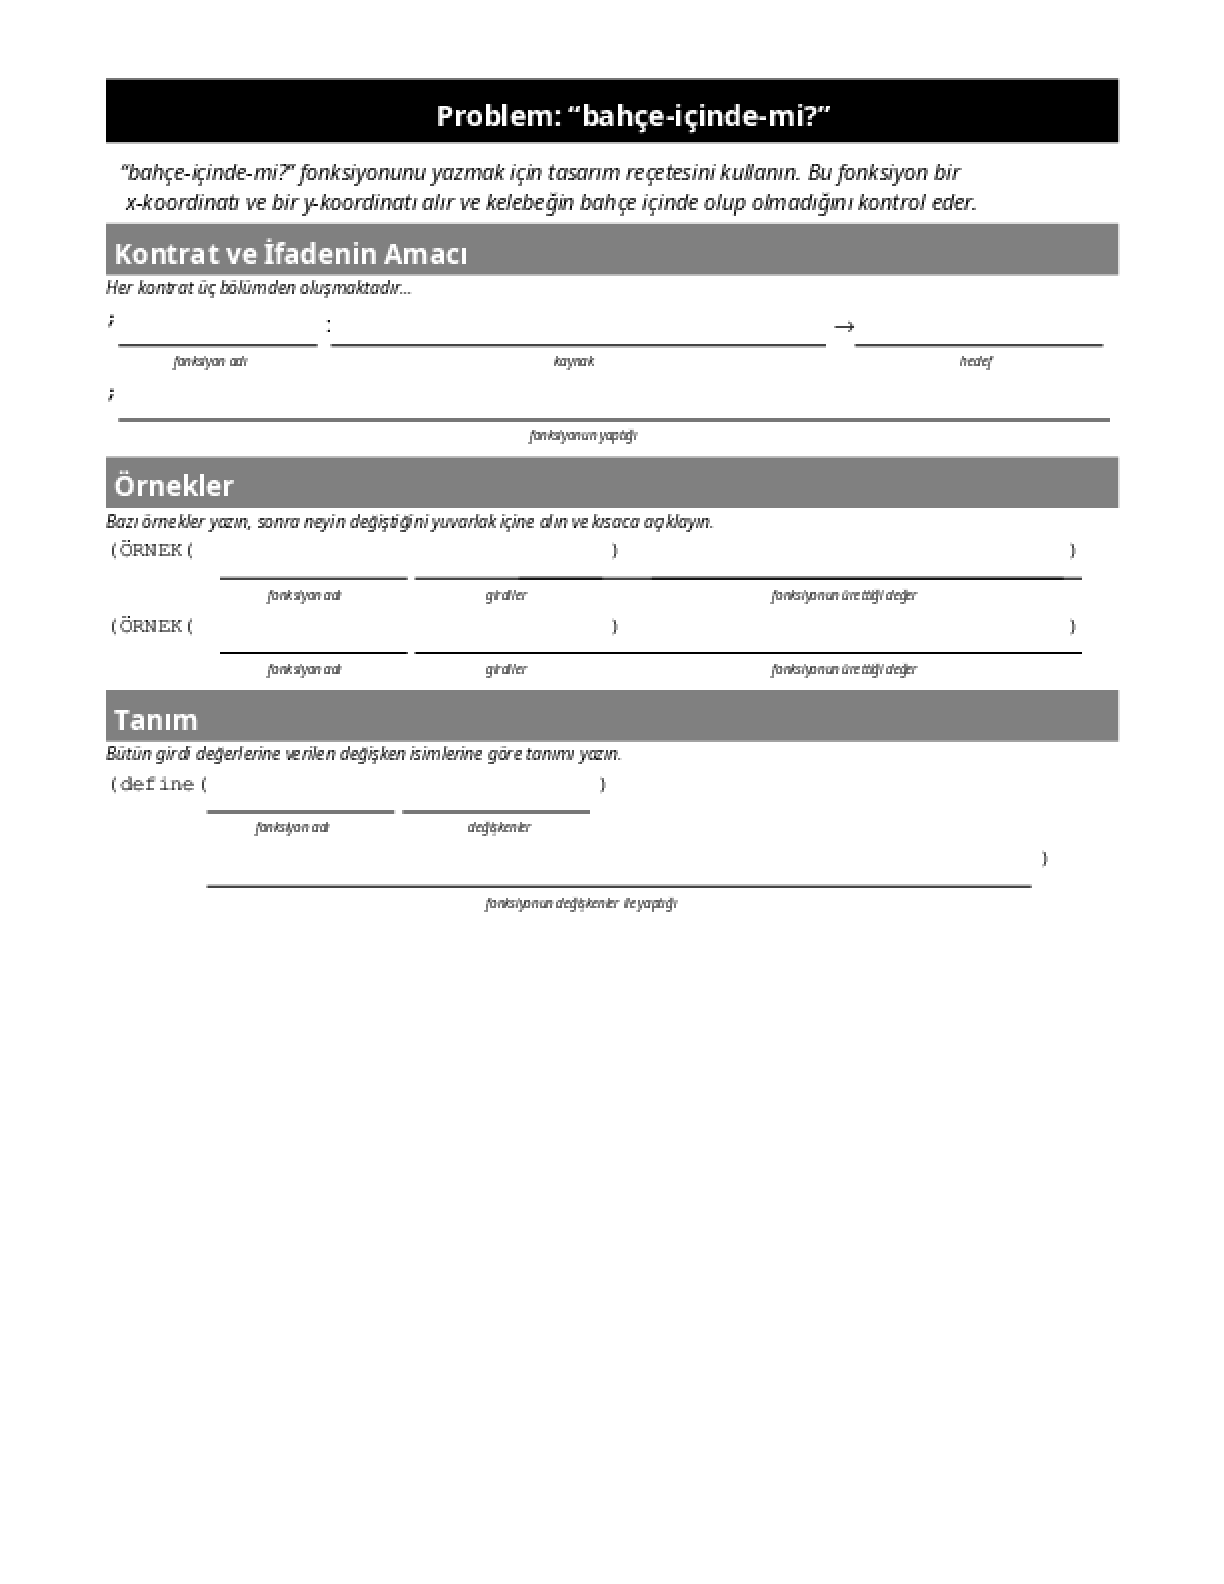
\includegraphics[width=1\linewidth]{cebirsplit-28.png}
\newpage
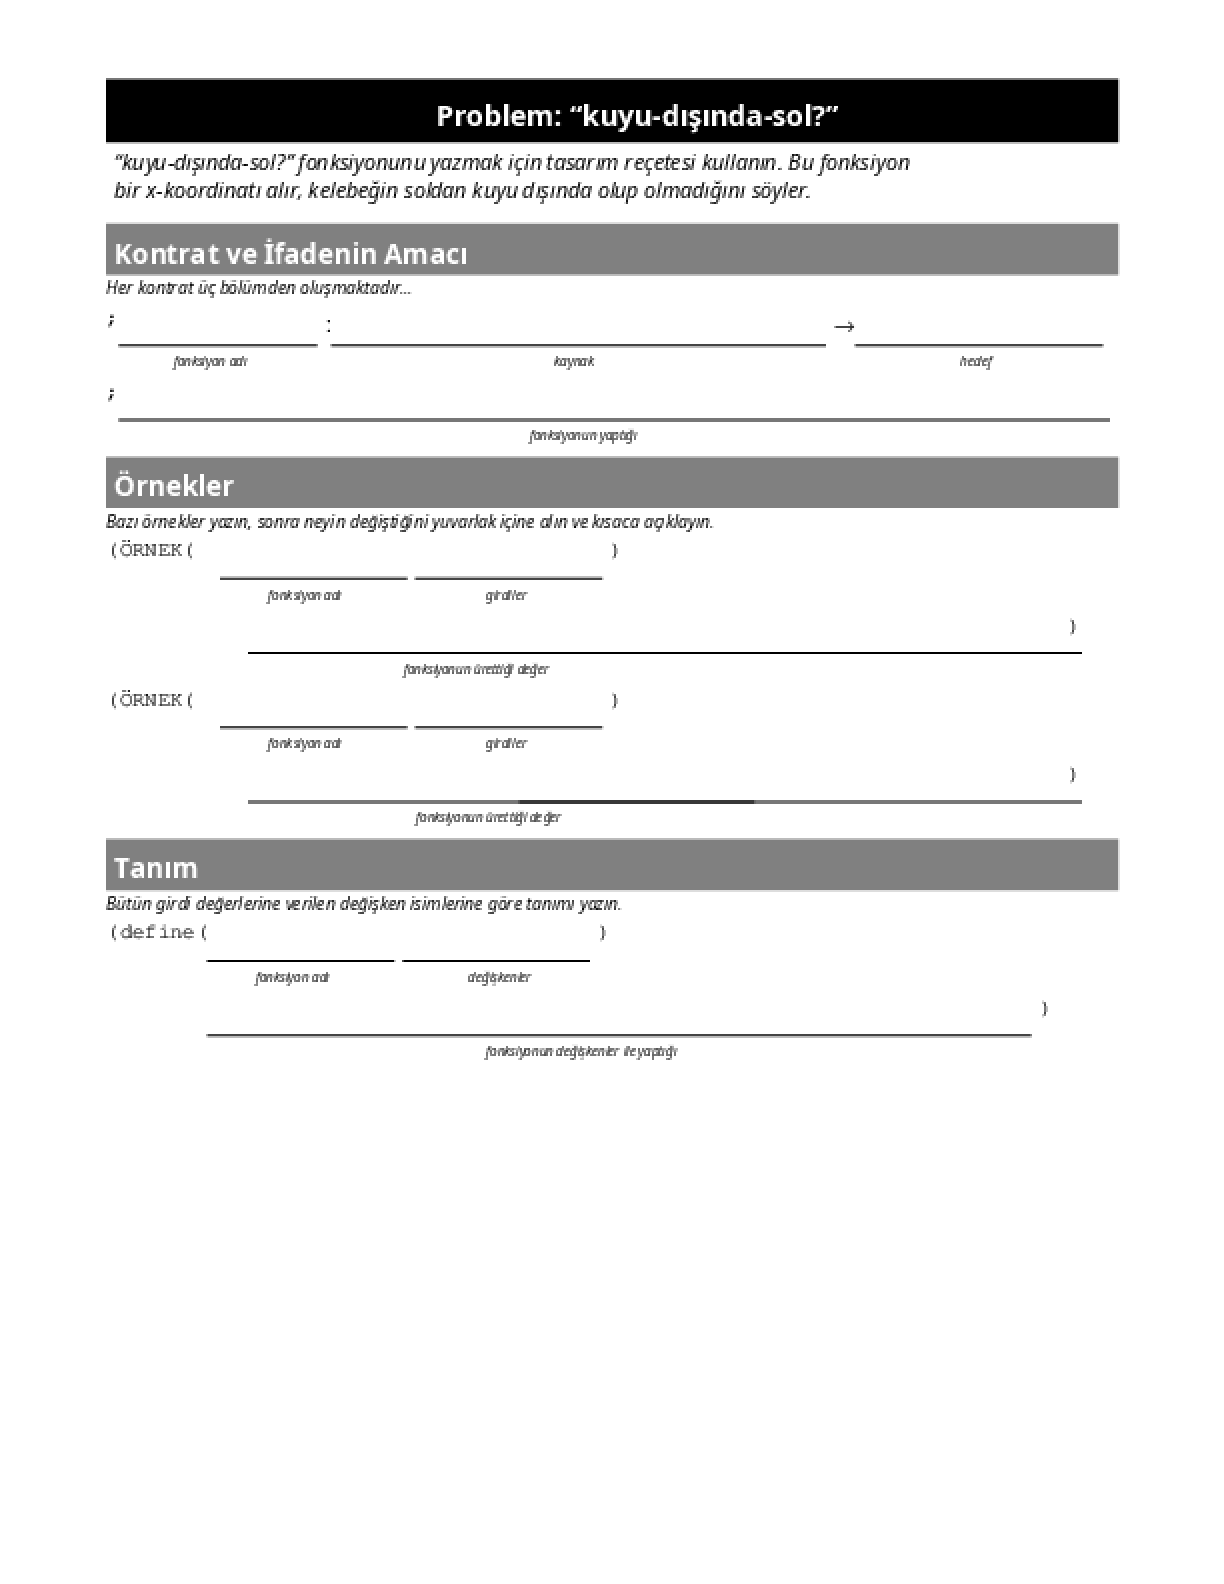
\includegraphics[width=1\linewidth]{cebirsplit-29.png}
\newpage
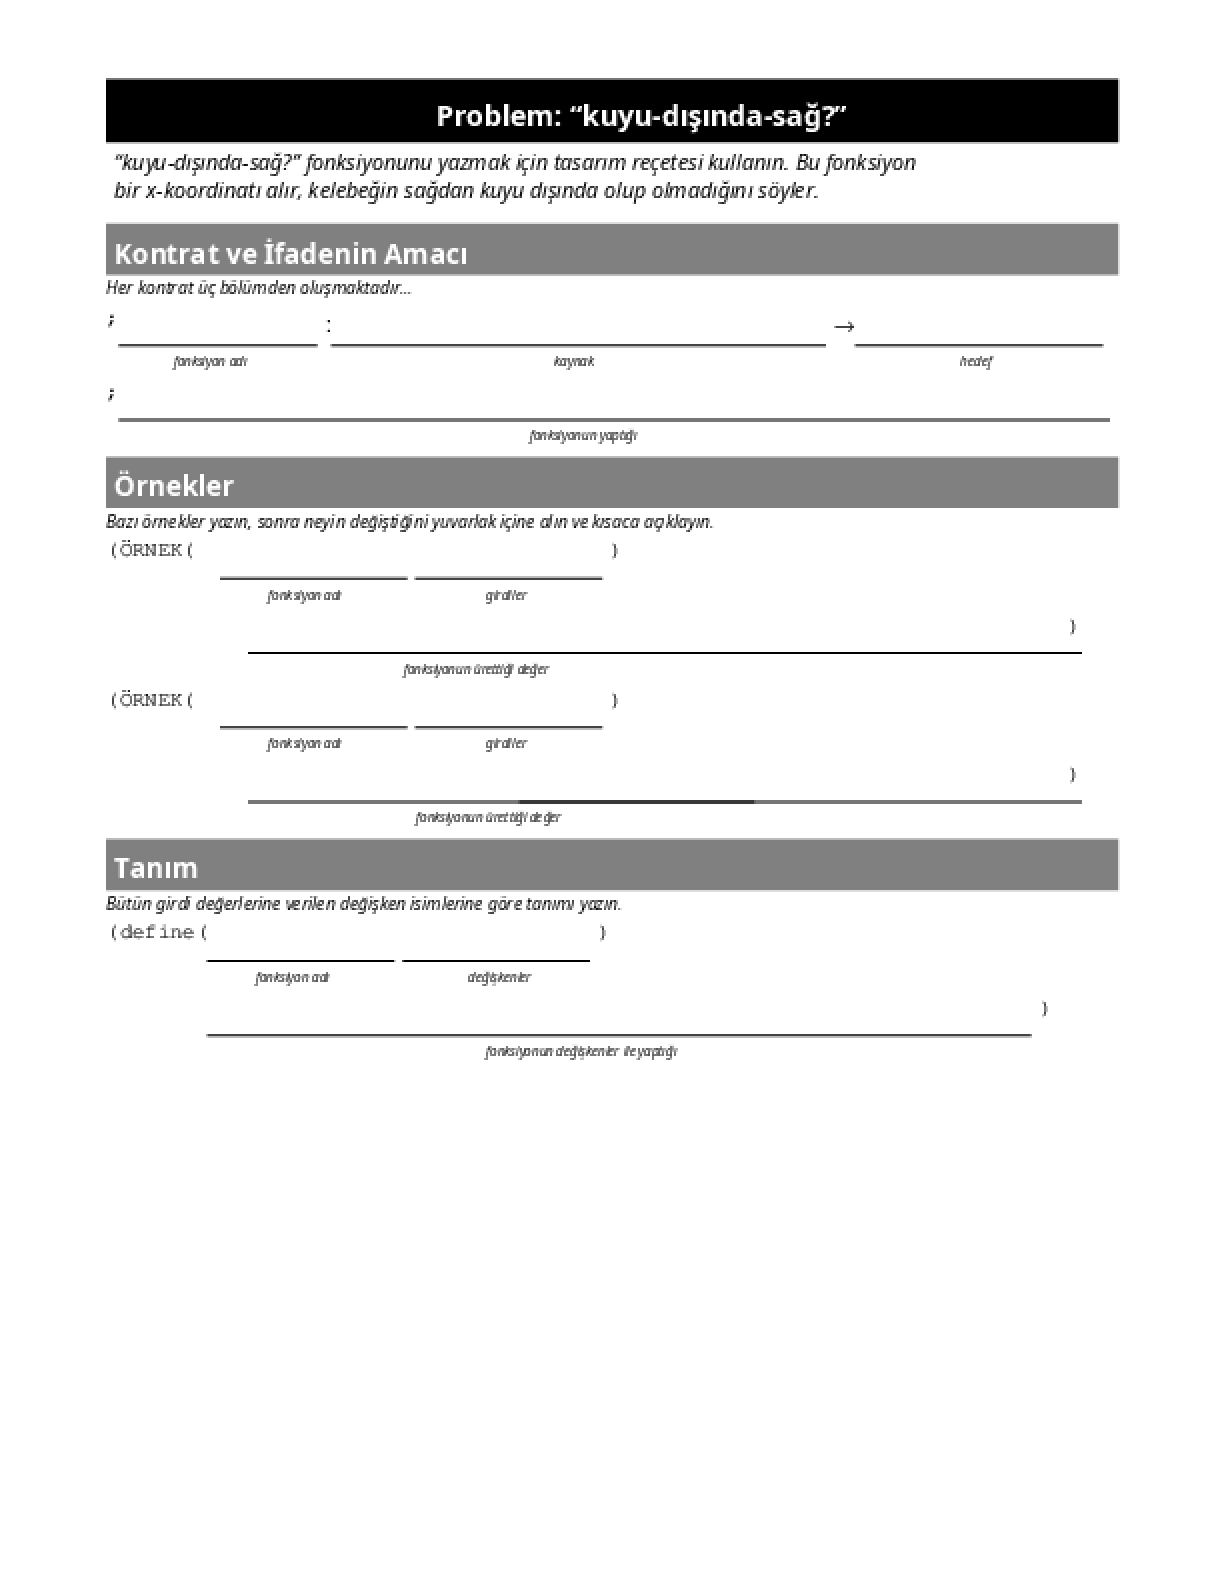
\includegraphics[width=1\linewidth]{cebirsplit-30.png}
\newpage
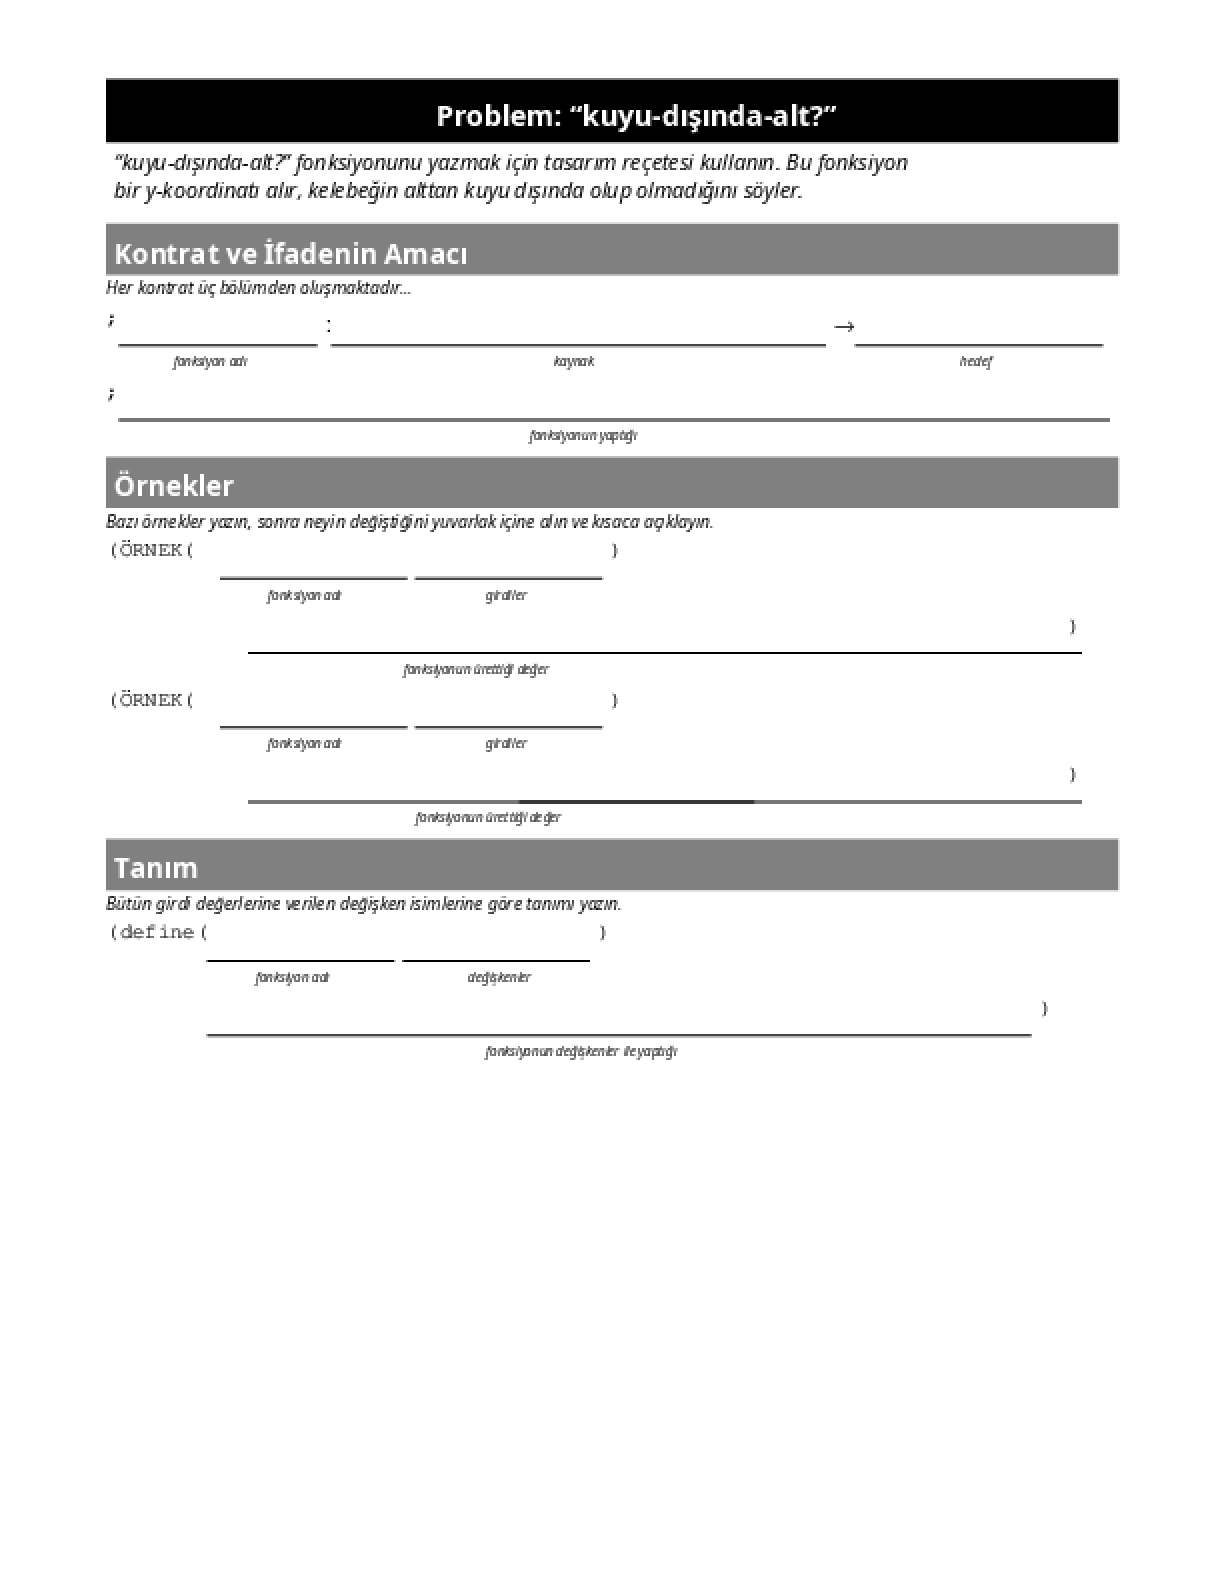
\includegraphics[width=1\linewidth]{cebirsplit-31.png}
\newpage
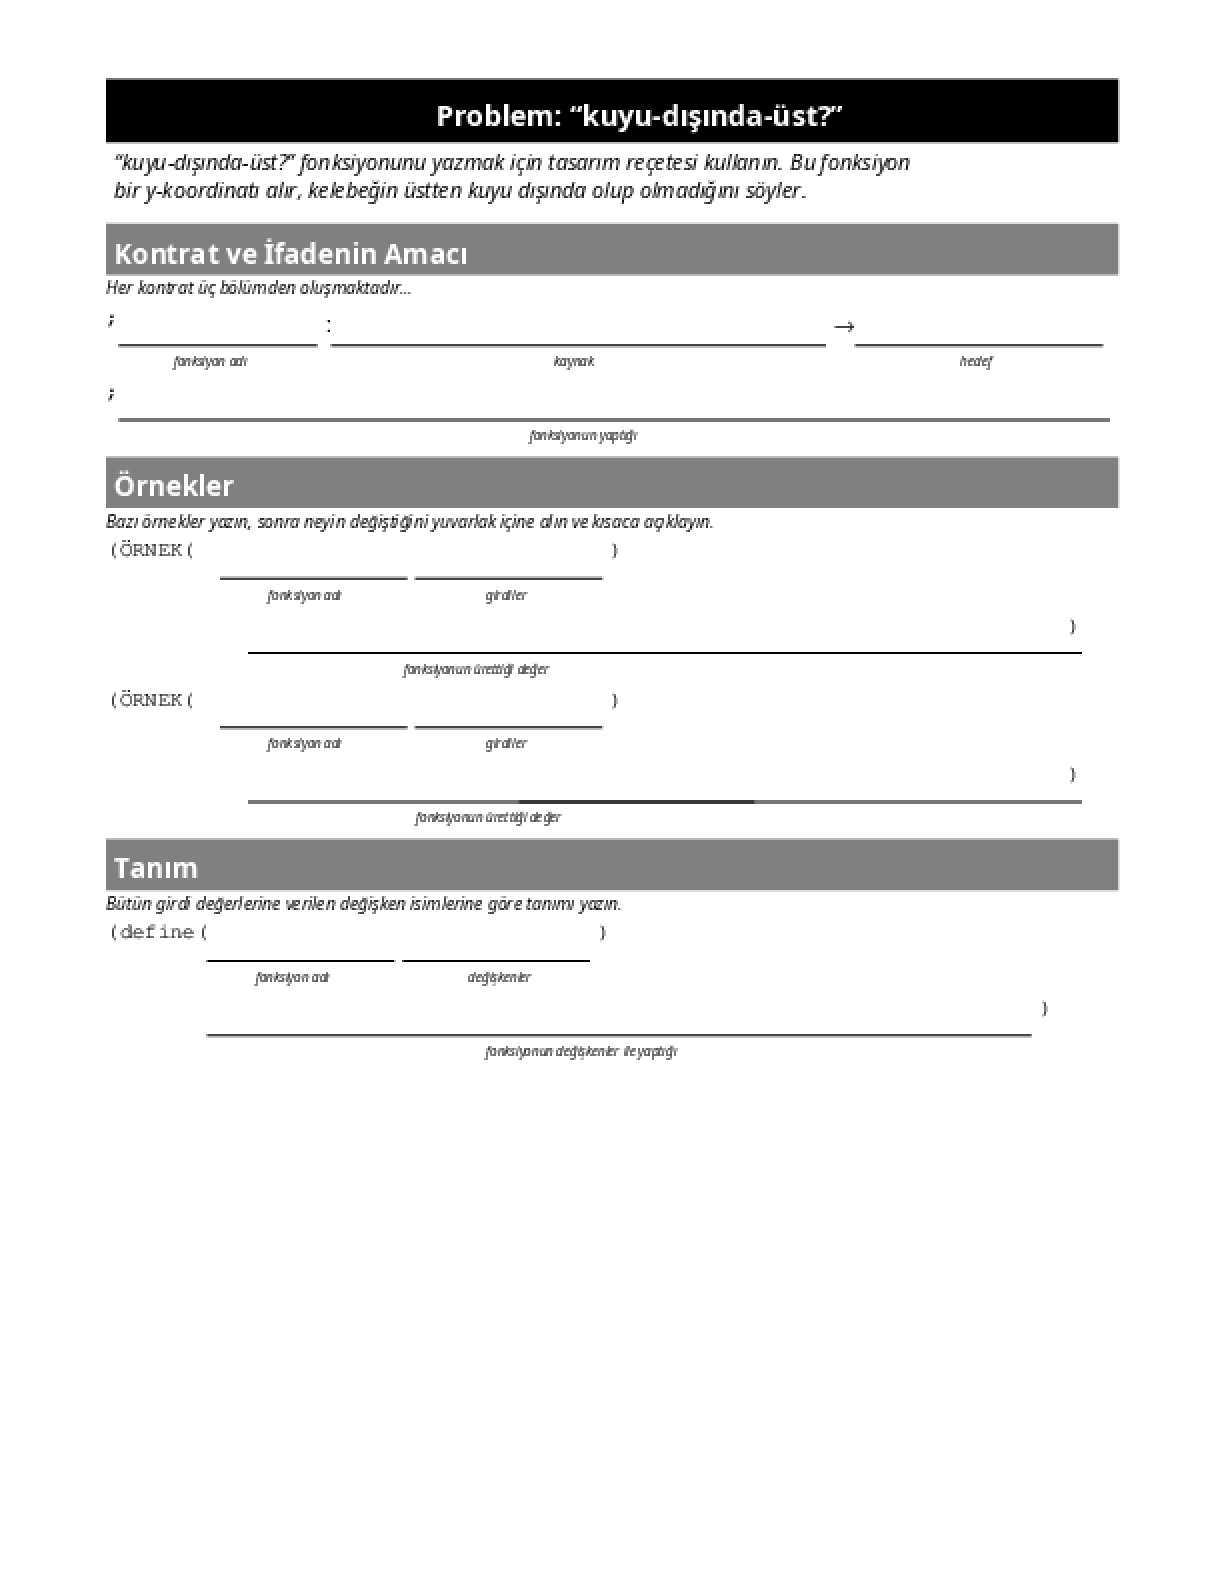
\includegraphics[width=1\linewidth]{cebirsplit-32.png}
\newpage
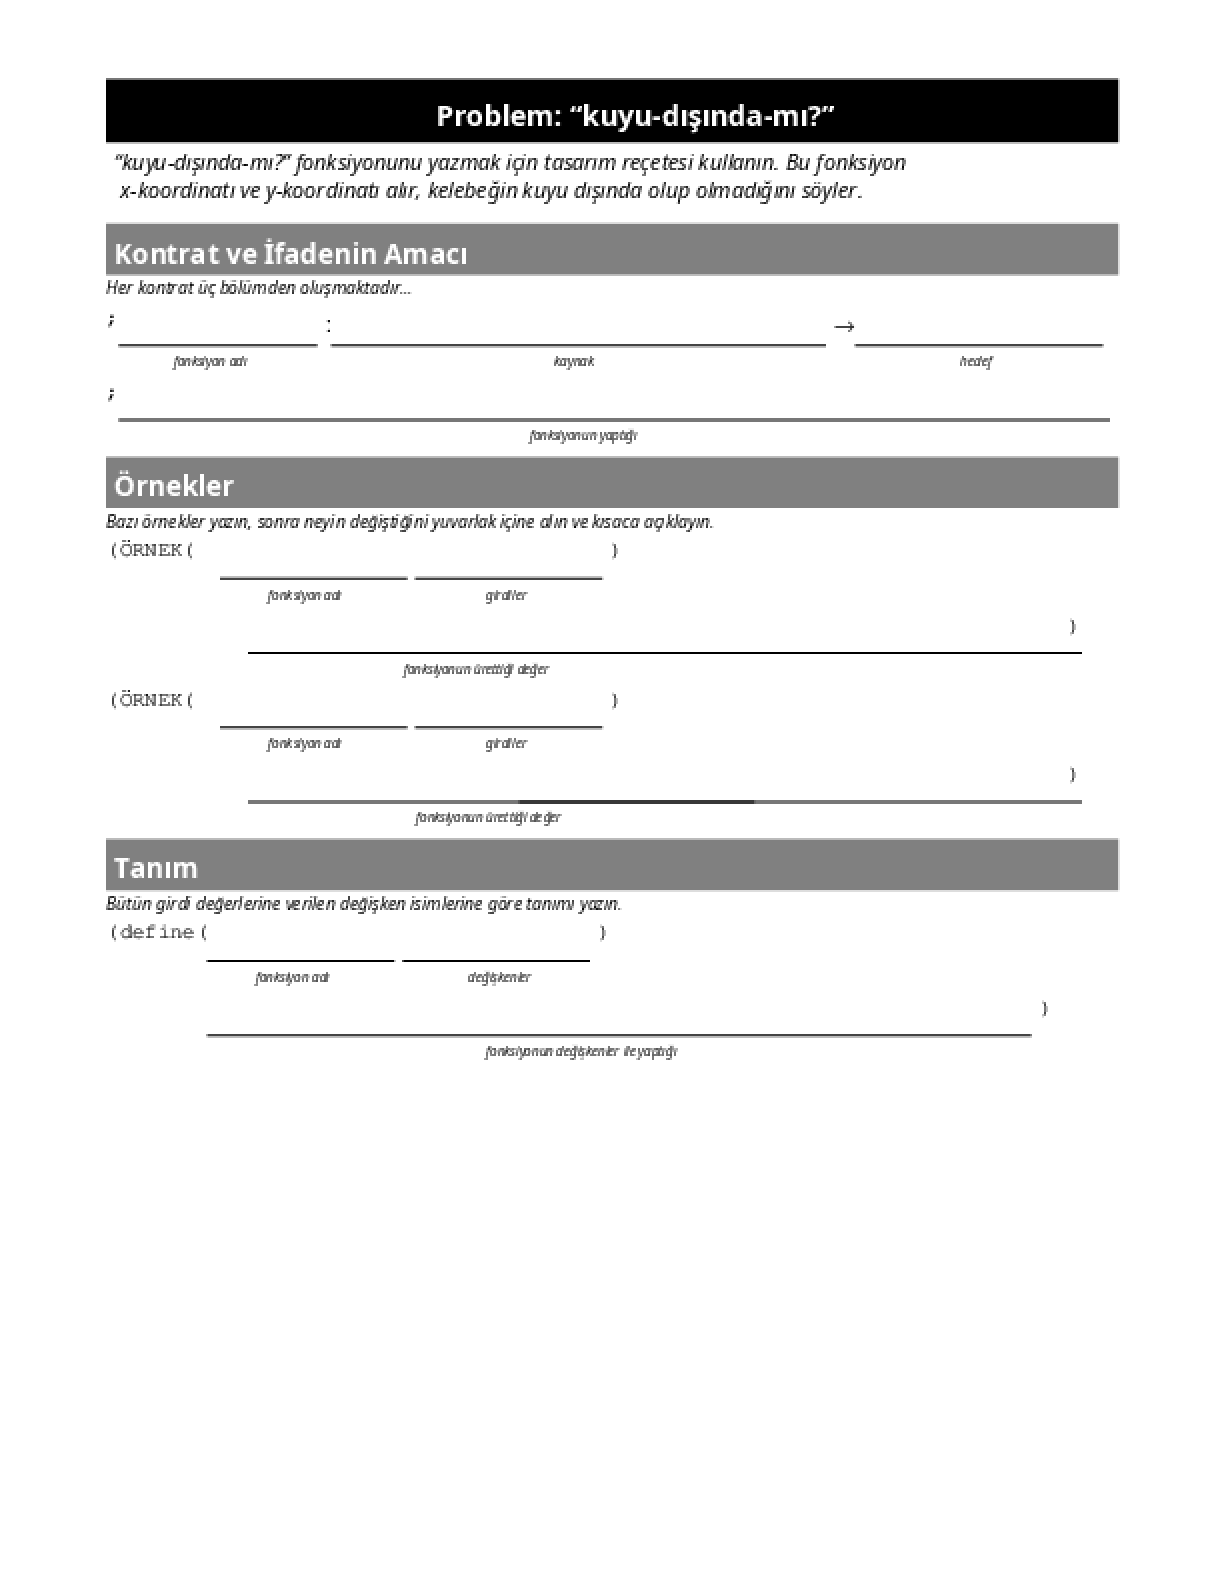
\includegraphics[width=1\linewidth]{cebirsplit-33.png}
\newpage
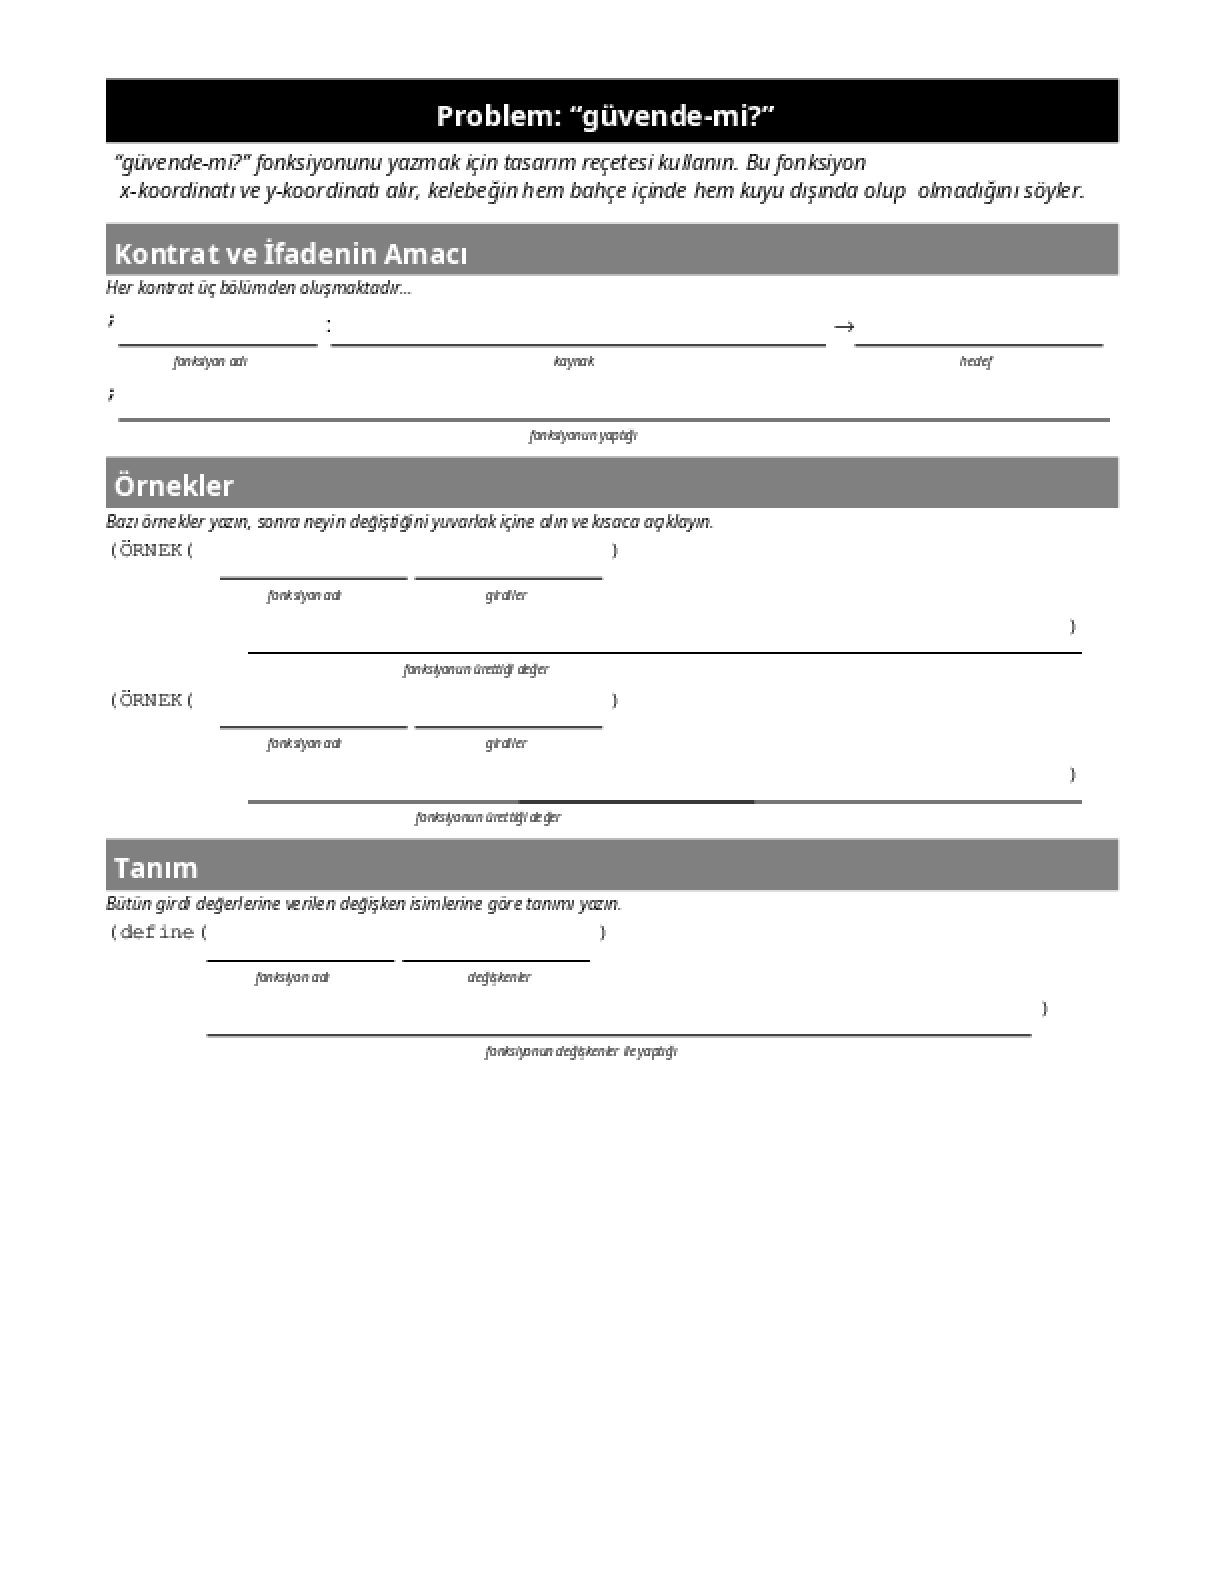
\includegraphics[width=1\linewidth]{cebirsplit-34.png}
\newpage
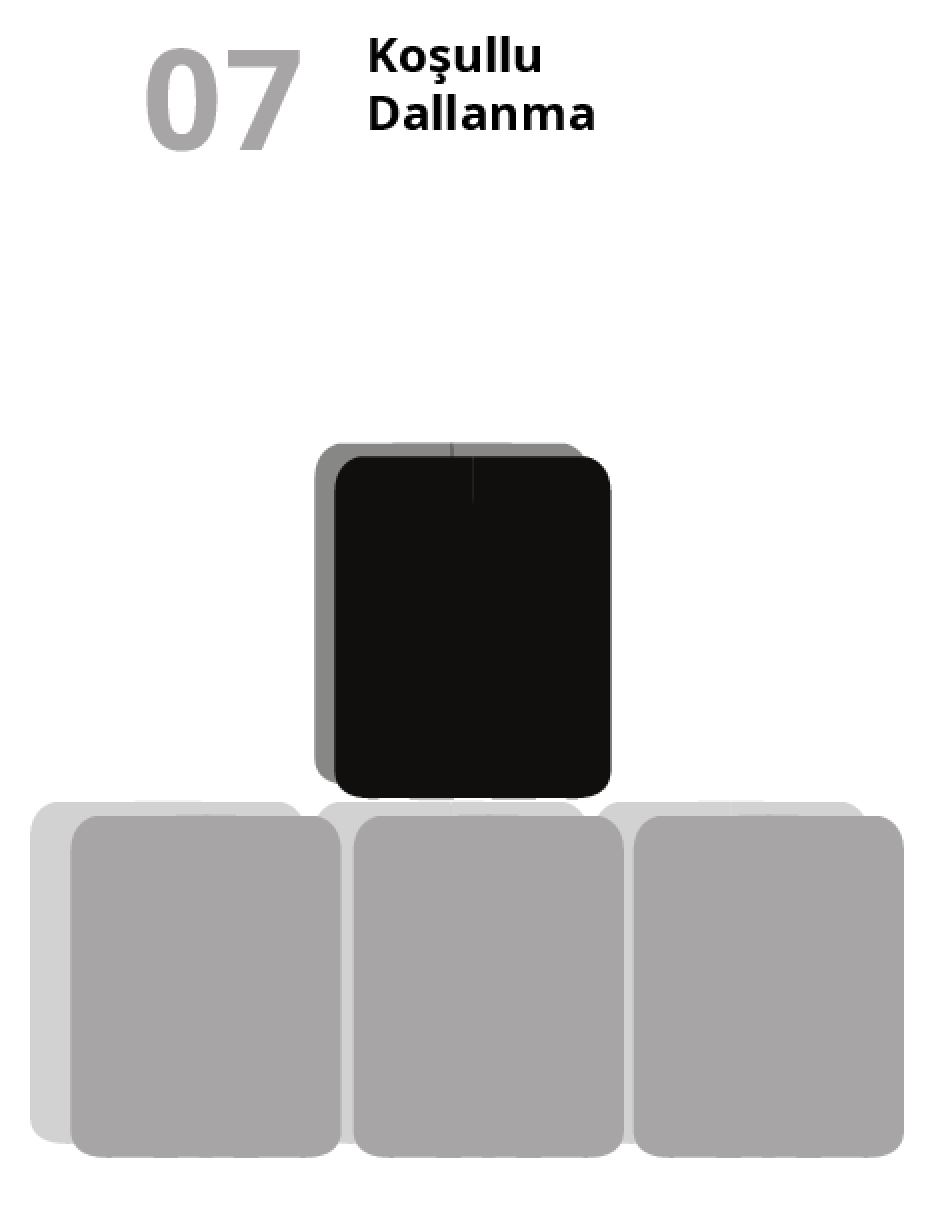
\includegraphics[width=1\linewidth]{cebir-bolum-07-000.png}
\newpage
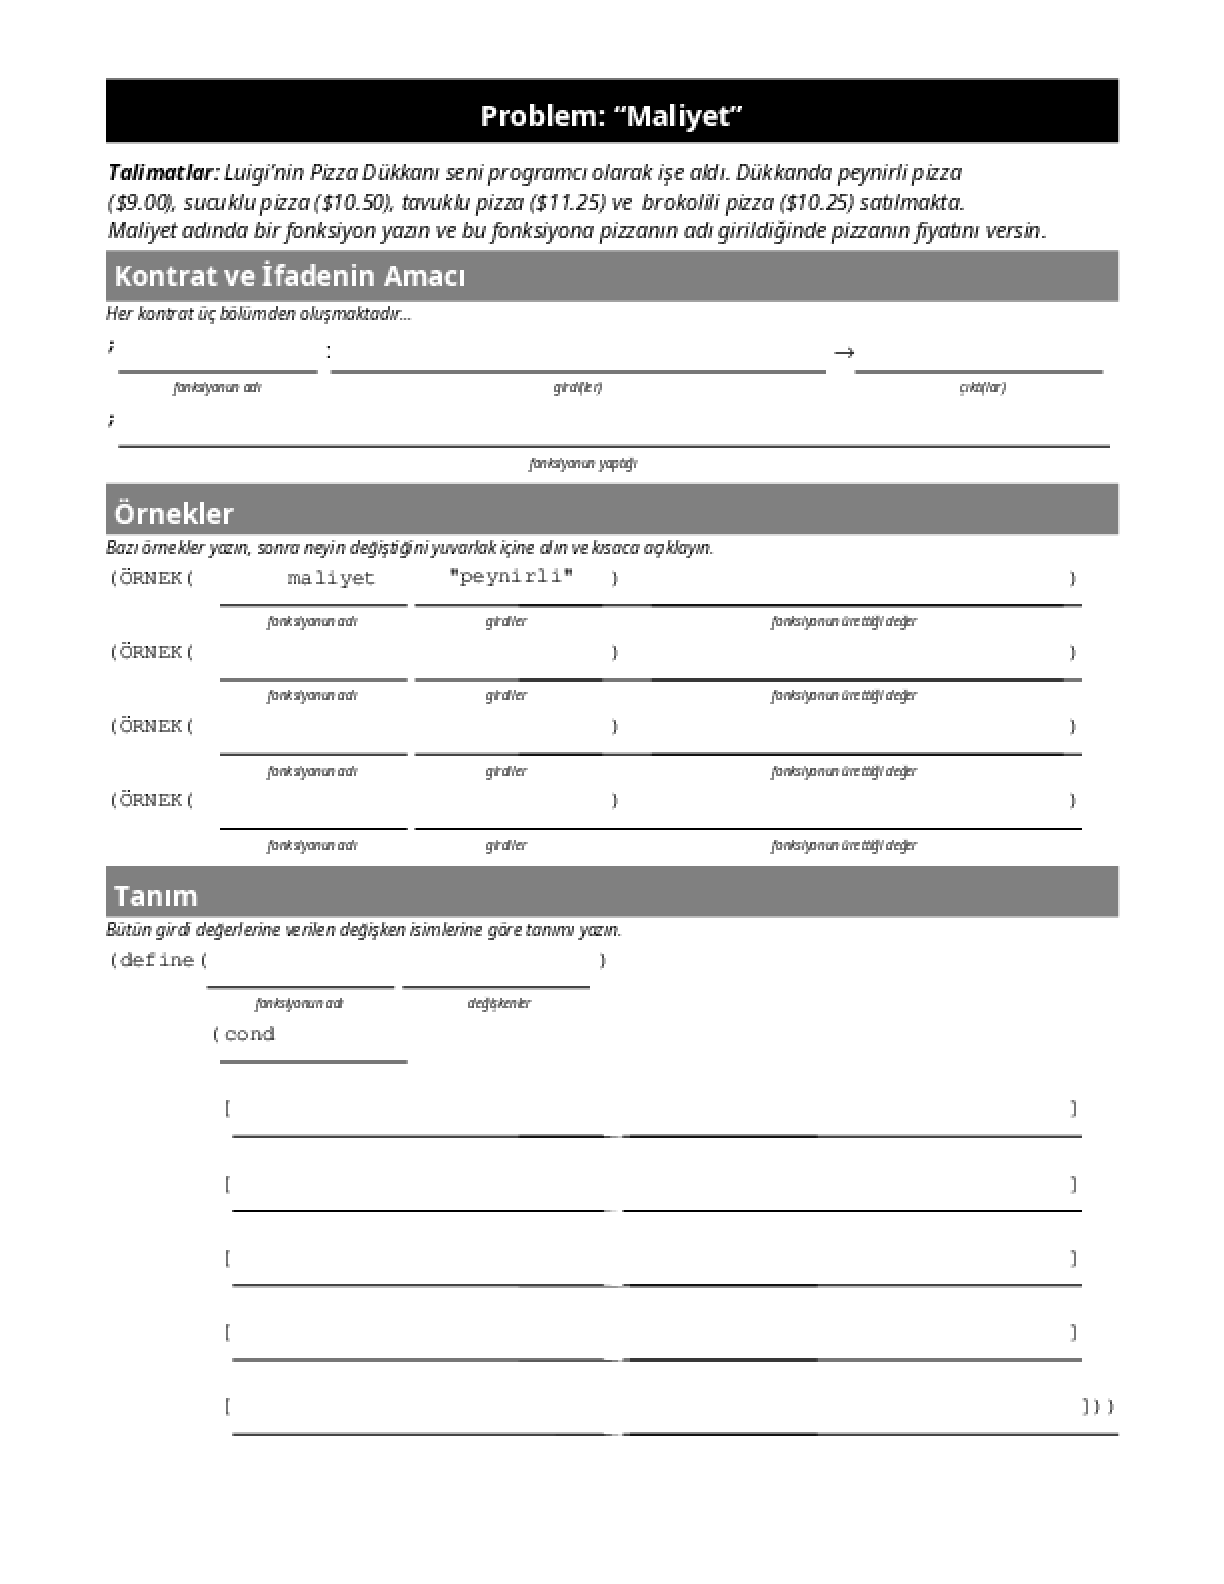
\includegraphics[width=1\linewidth]{cebirsplit-36.png}
\newpage
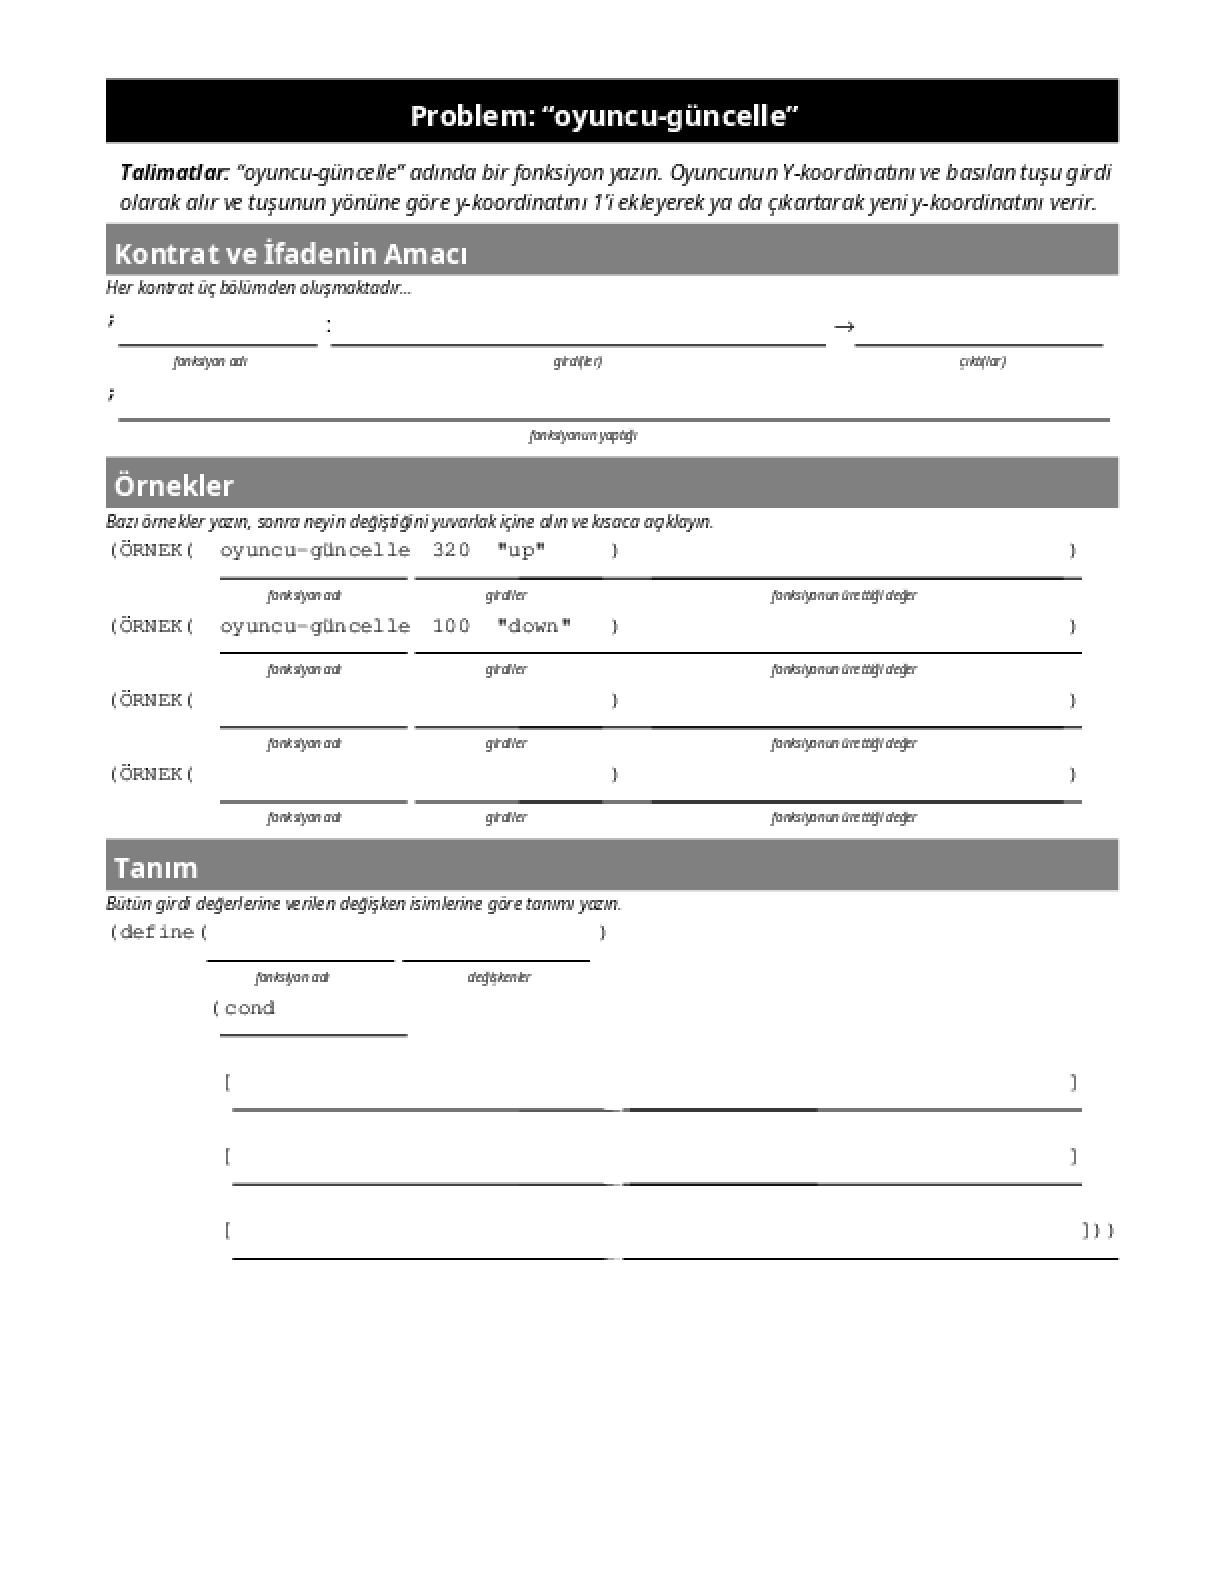
\includegraphics[width=1\linewidth]{cebirsplit-37.png}
\newpage
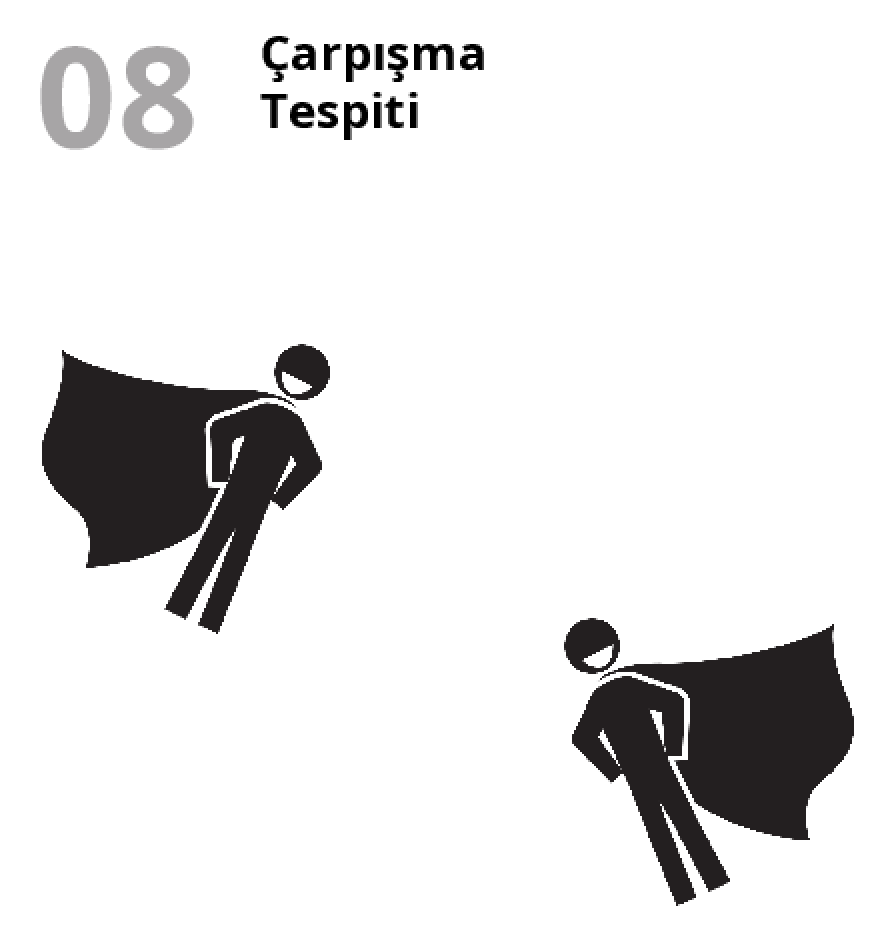
\includegraphics[width=1\linewidth]{cebir-bolum-08-000.png}
\newpage
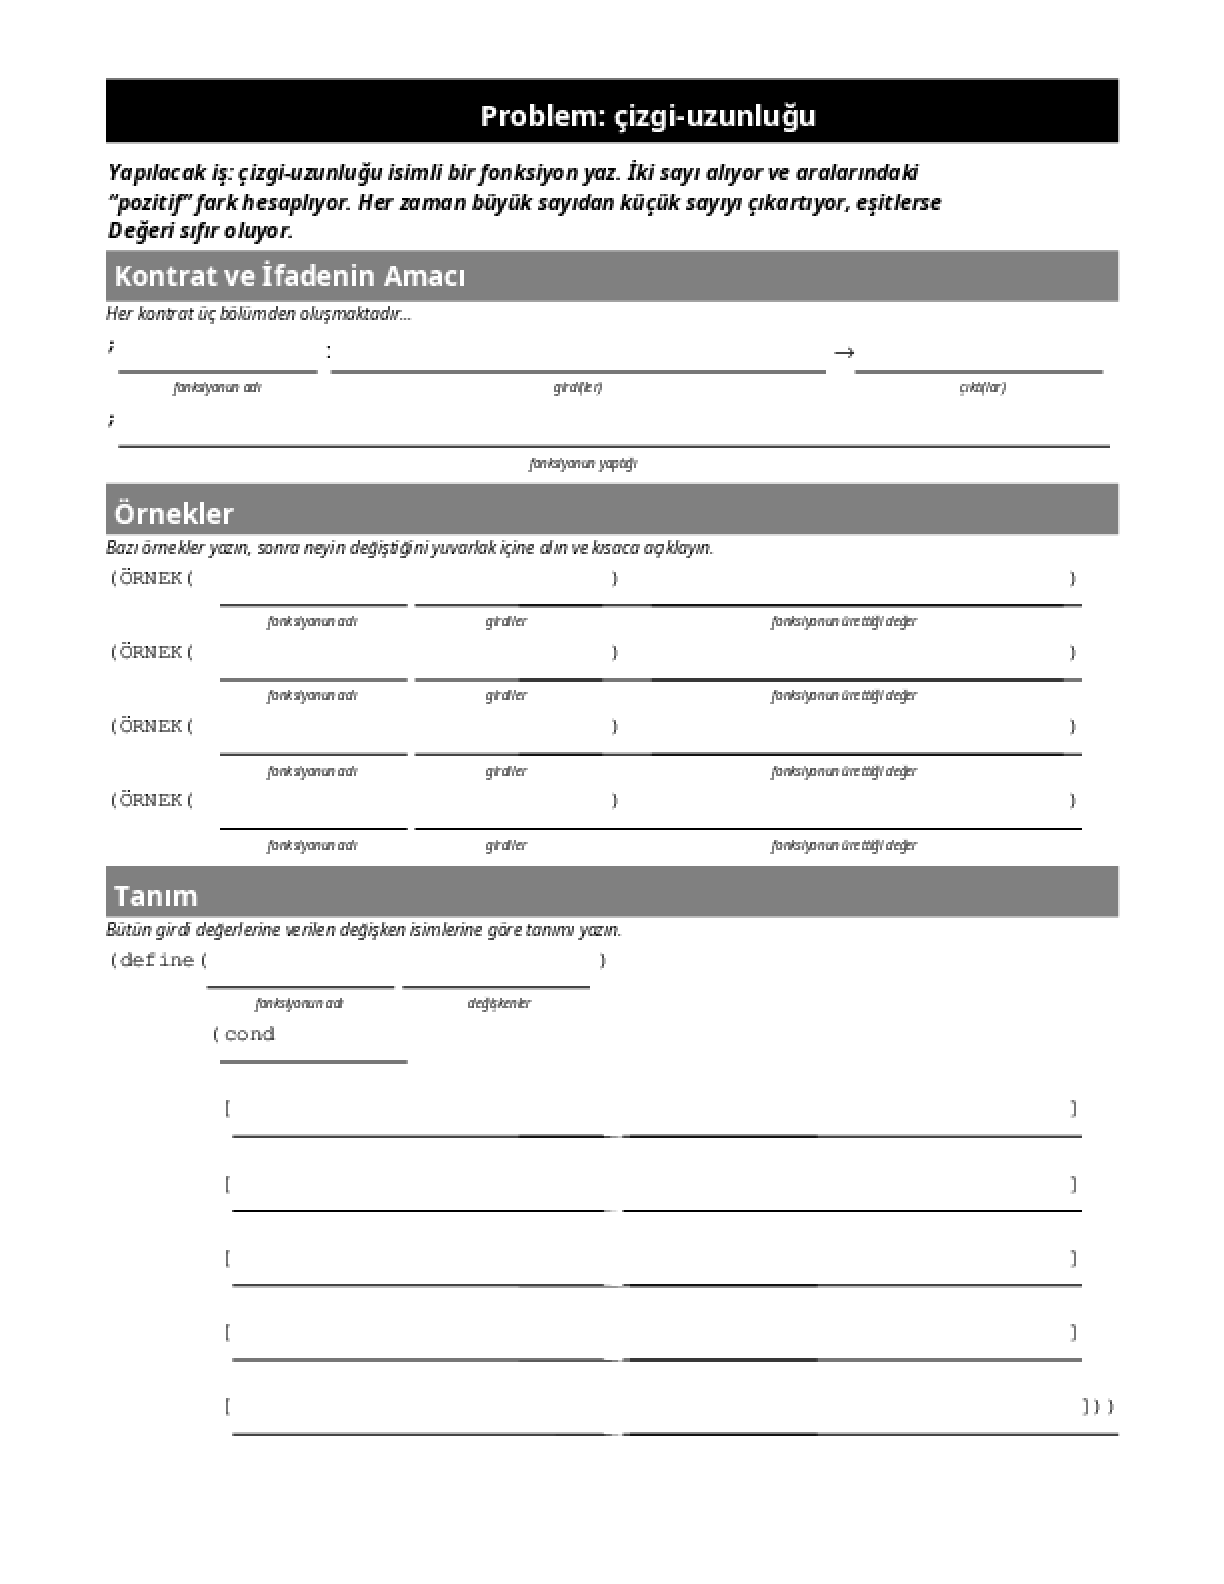
\includegraphics[width=1\linewidth]{cebirsplit-39.png}
\newpage
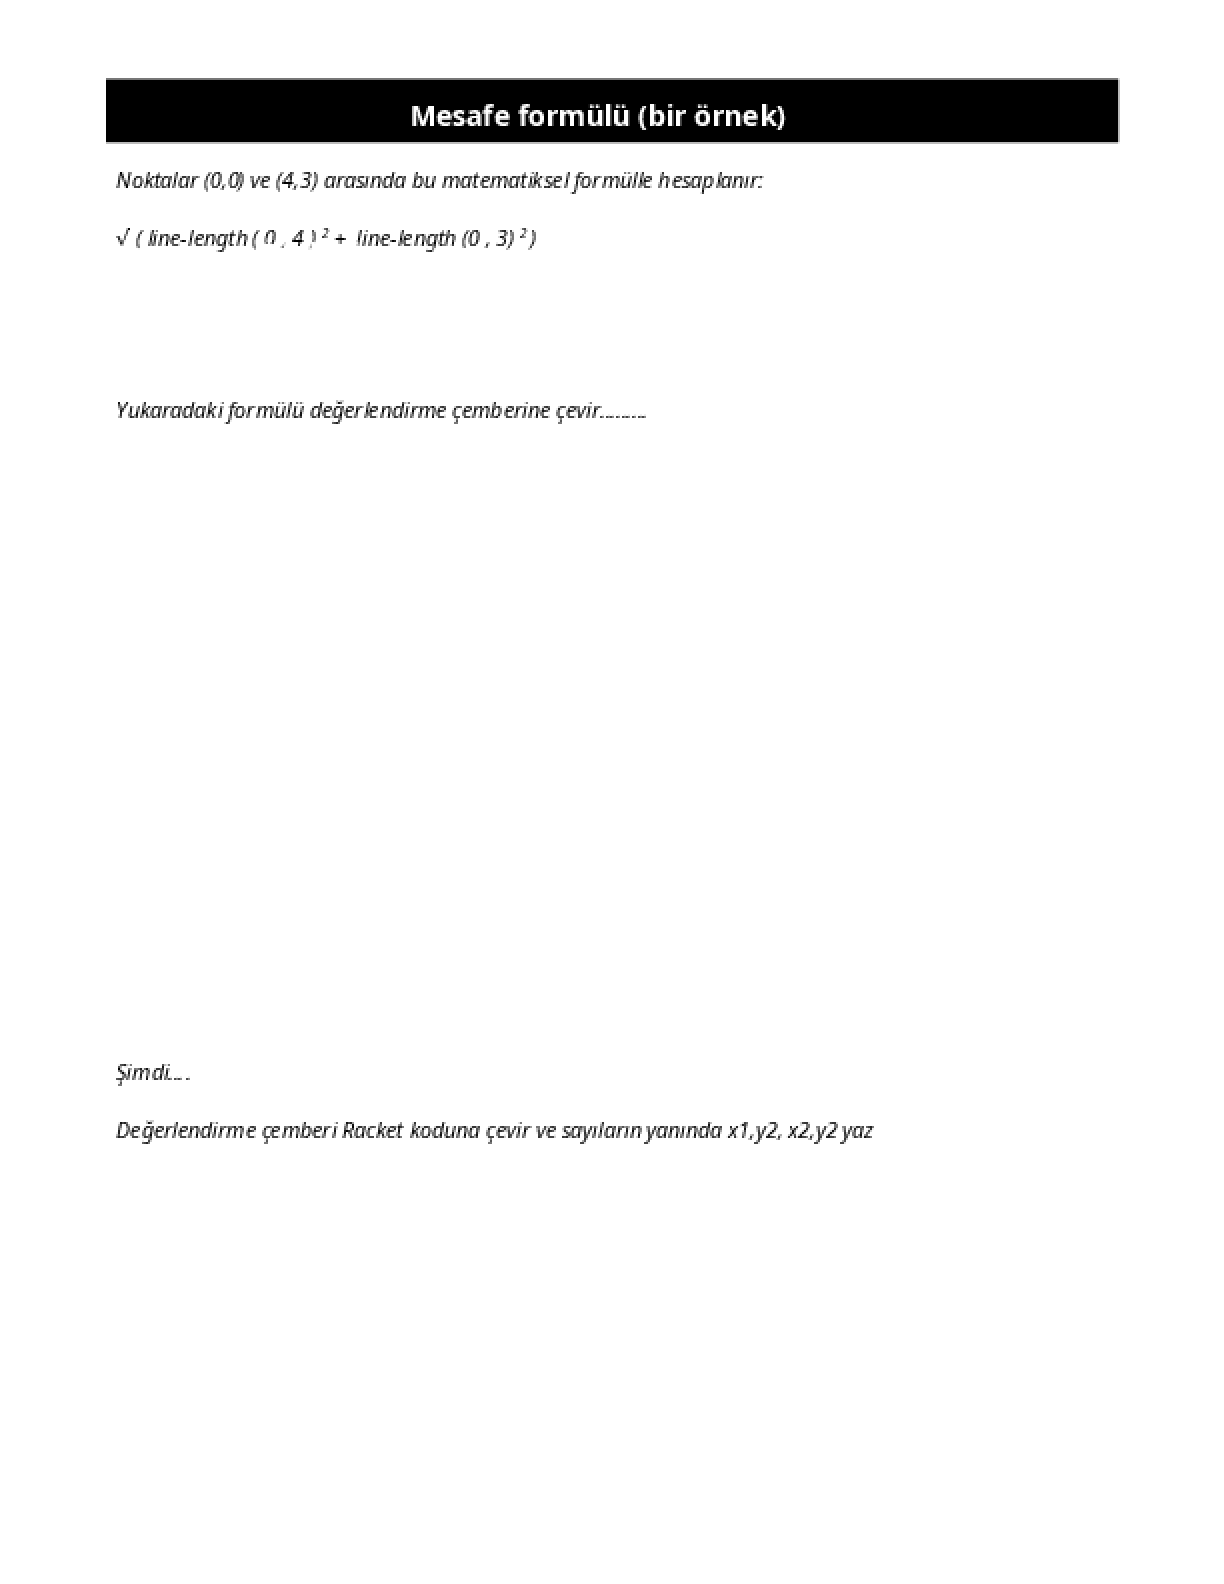
\includegraphics[width=1\linewidth]{cebirsplit-40.png}
\newpage
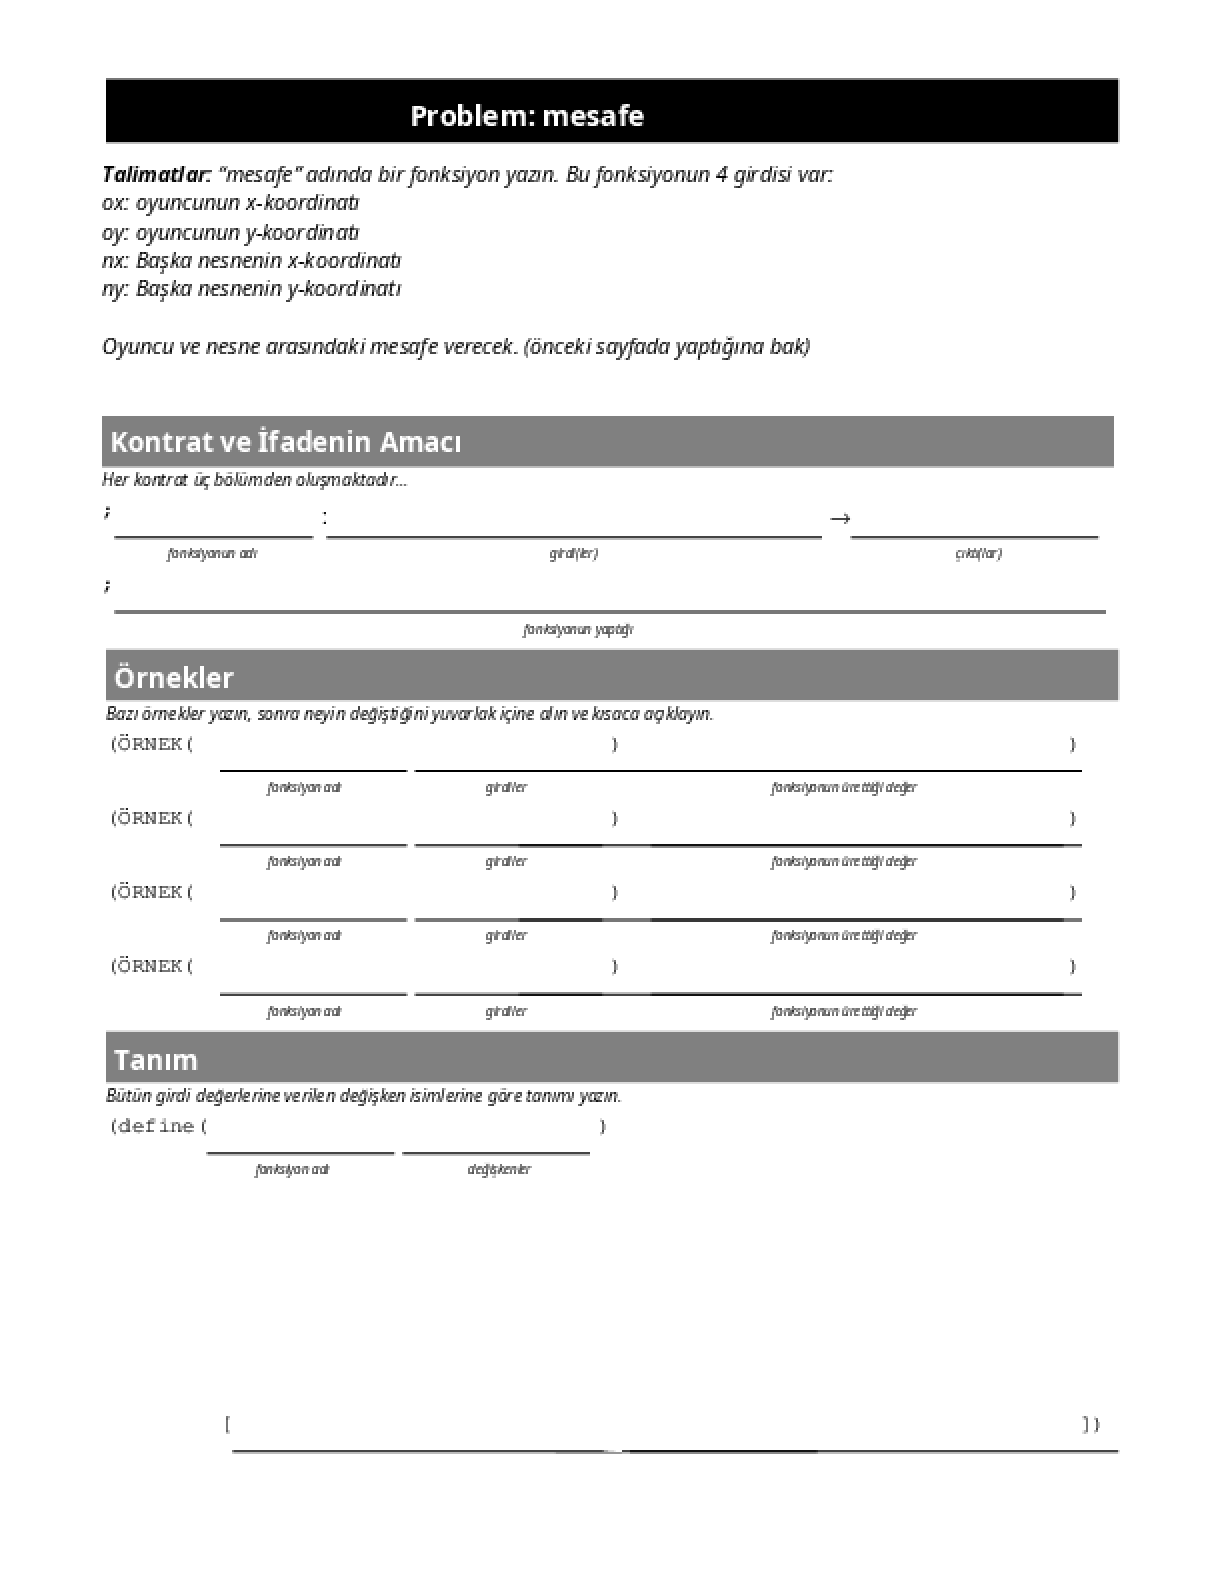
\includegraphics[width=1\linewidth]{cebirsplit-41.png}
\newpage
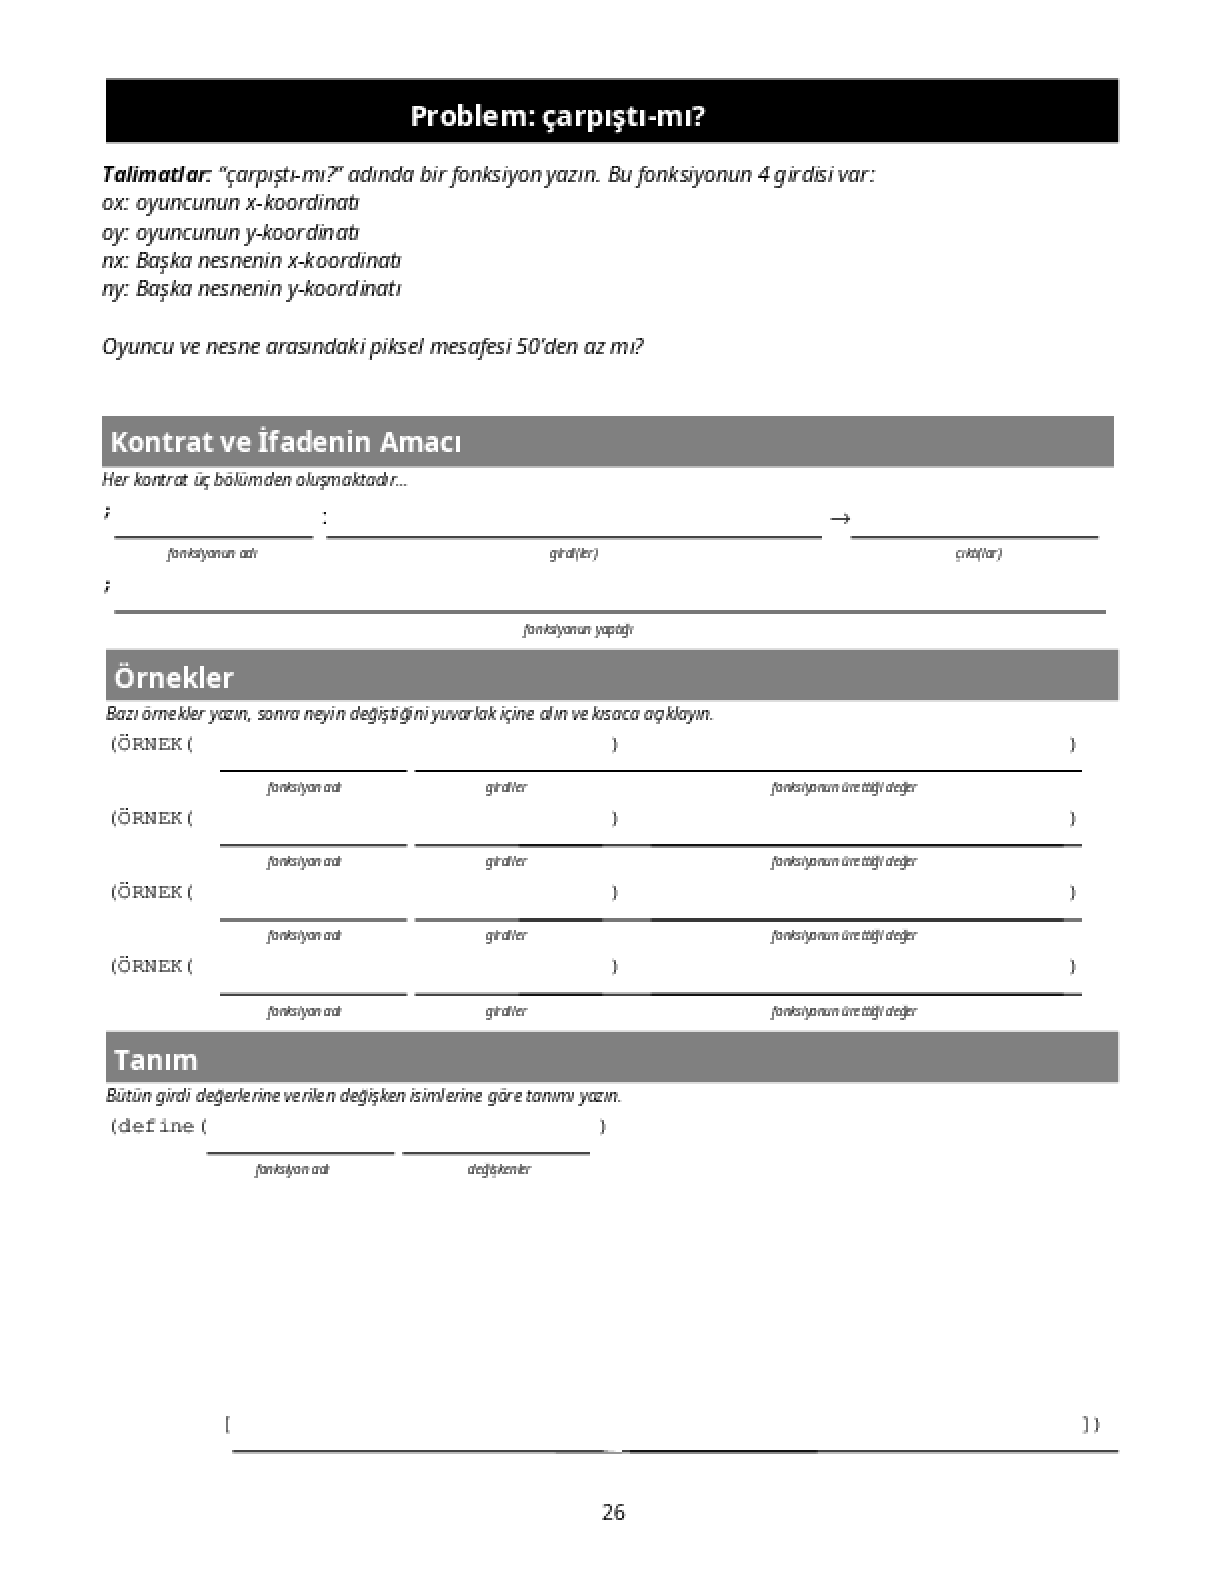
\includegraphics[width=1\linewidth]{cebirsplit-42.png}
\newpage
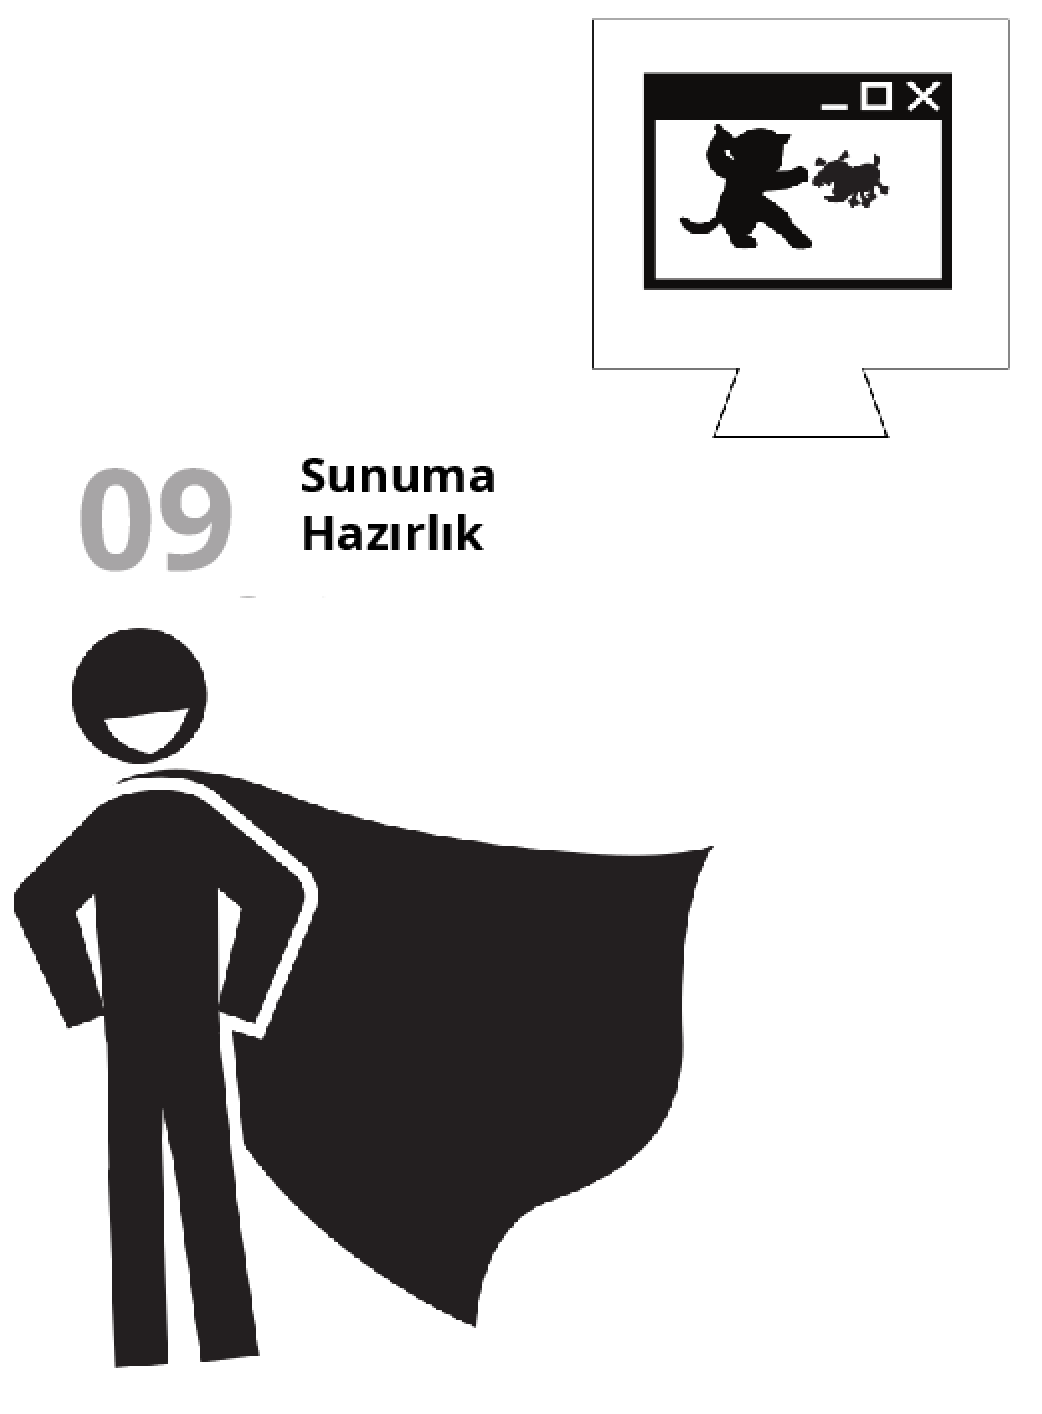
\includegraphics[width=1\linewidth]{cebir-bolum-09-000.png}
\newpage
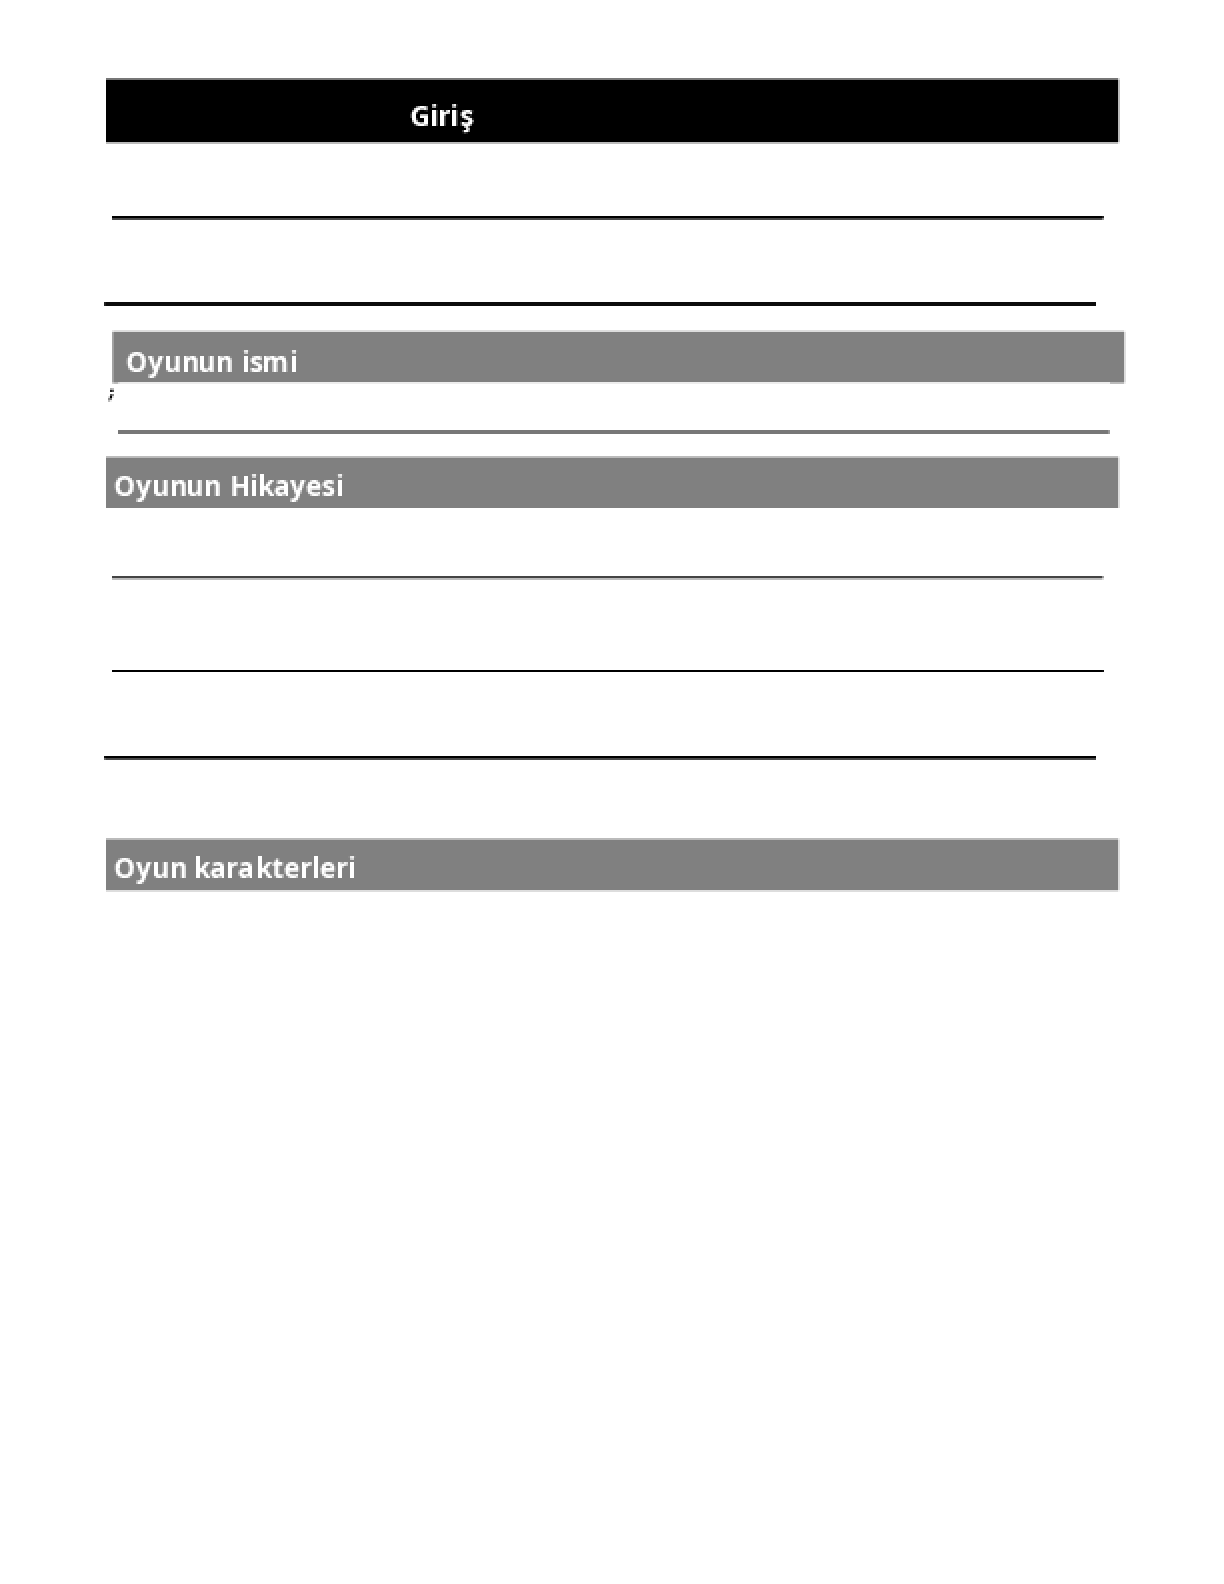
\includegraphics[width=1\linewidth]{cebirsplit-44.png}
\newpage
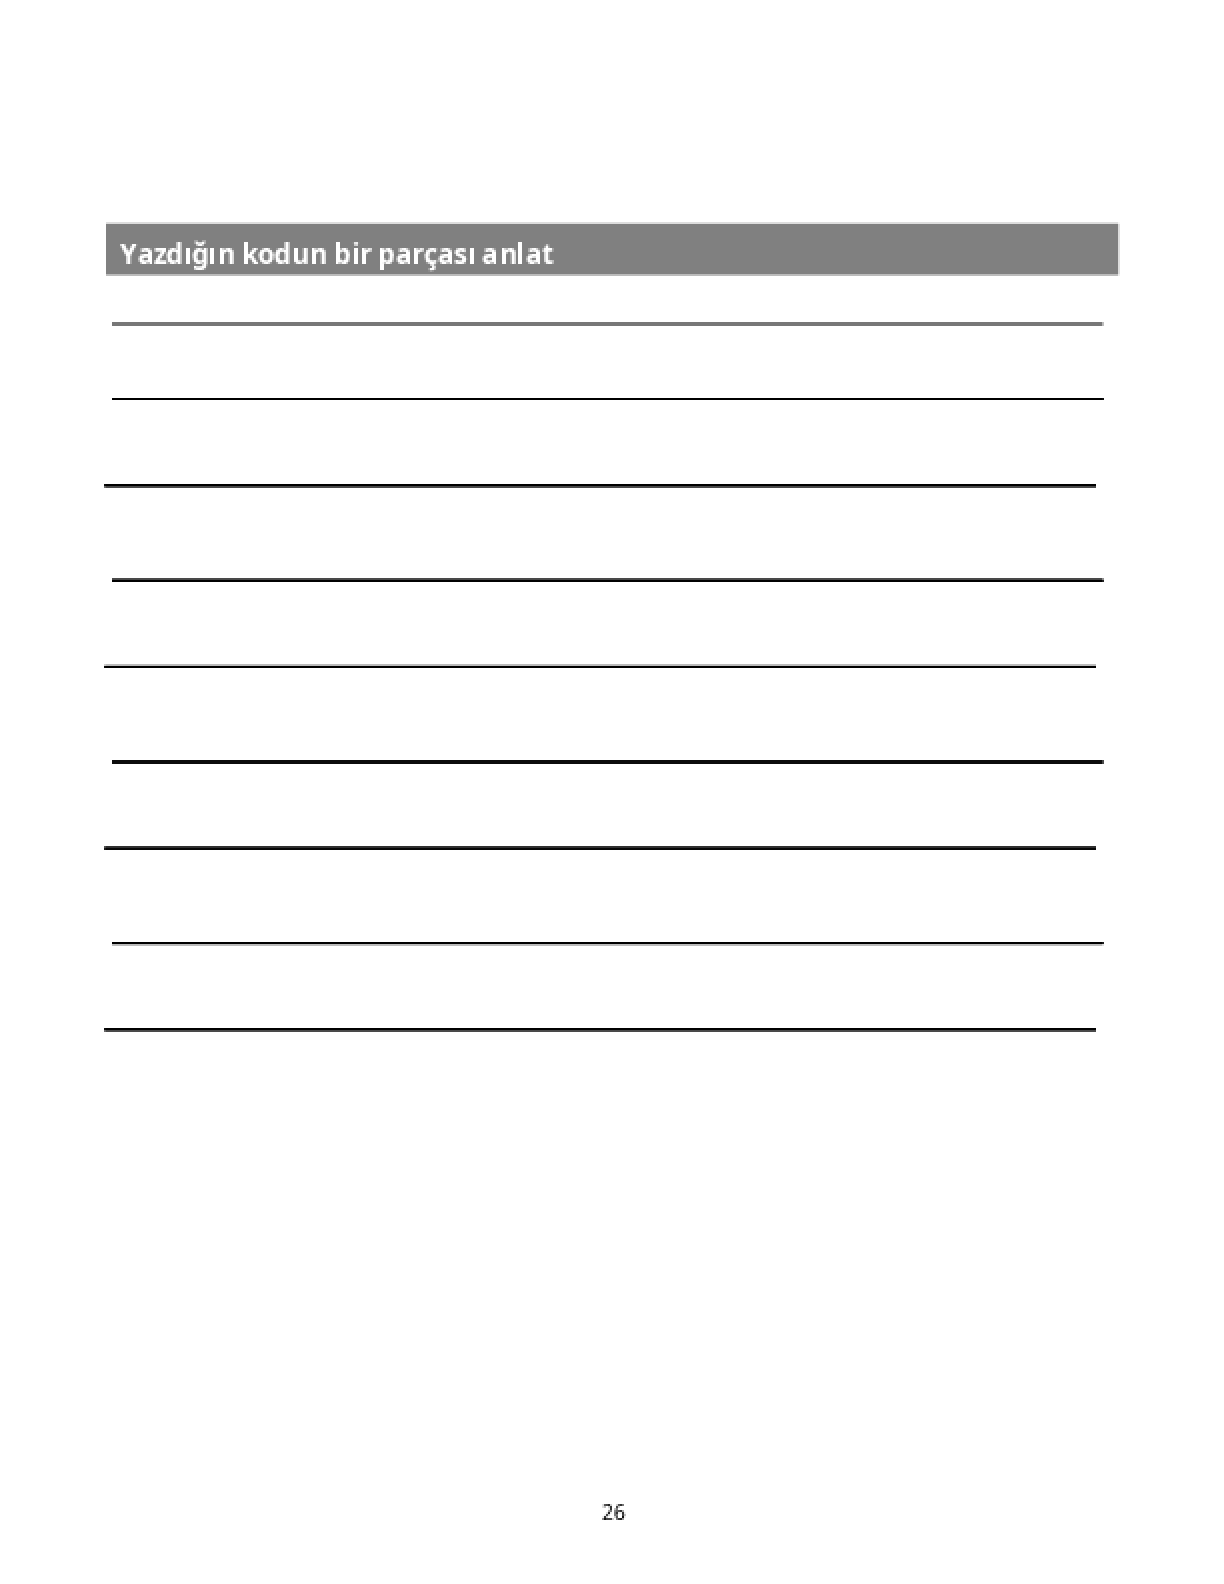
\includegraphics[width=1\linewidth]{cebirsplit-45.png}
\newpage
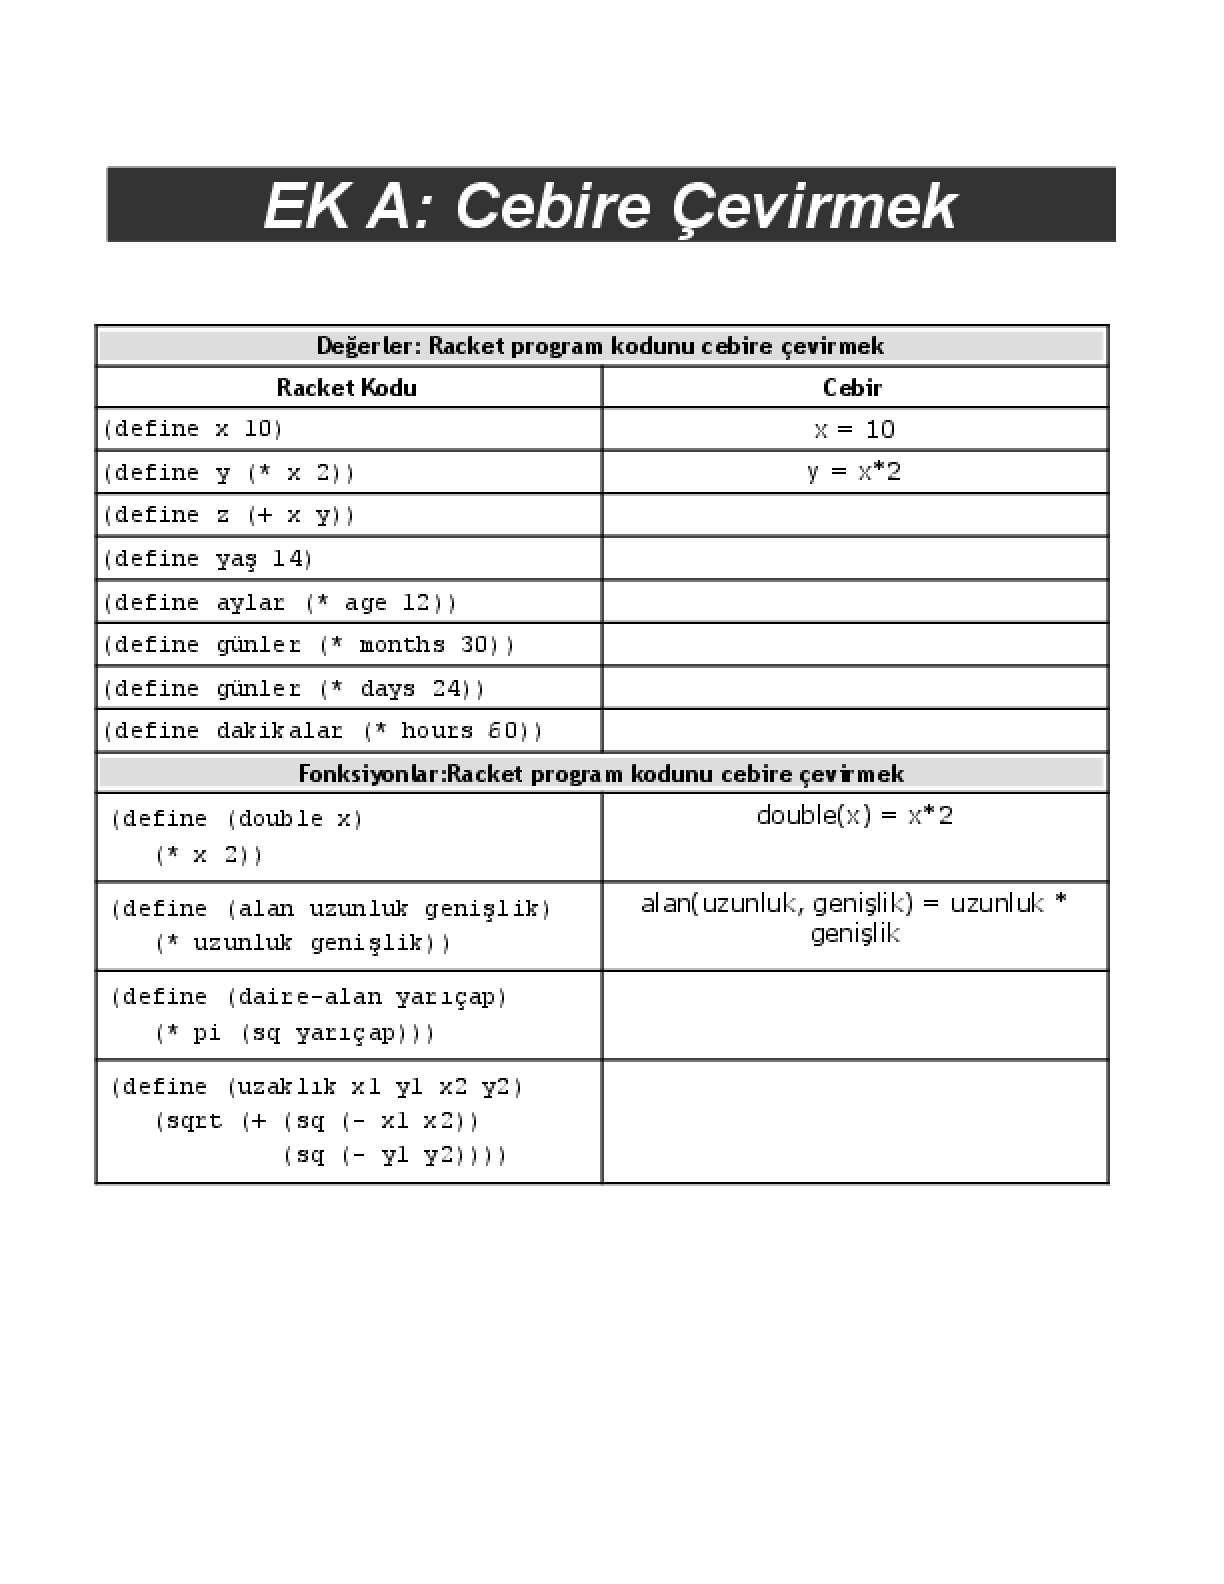
\includegraphics[width=1\linewidth]{cebirsplit-46.png}
\newpage
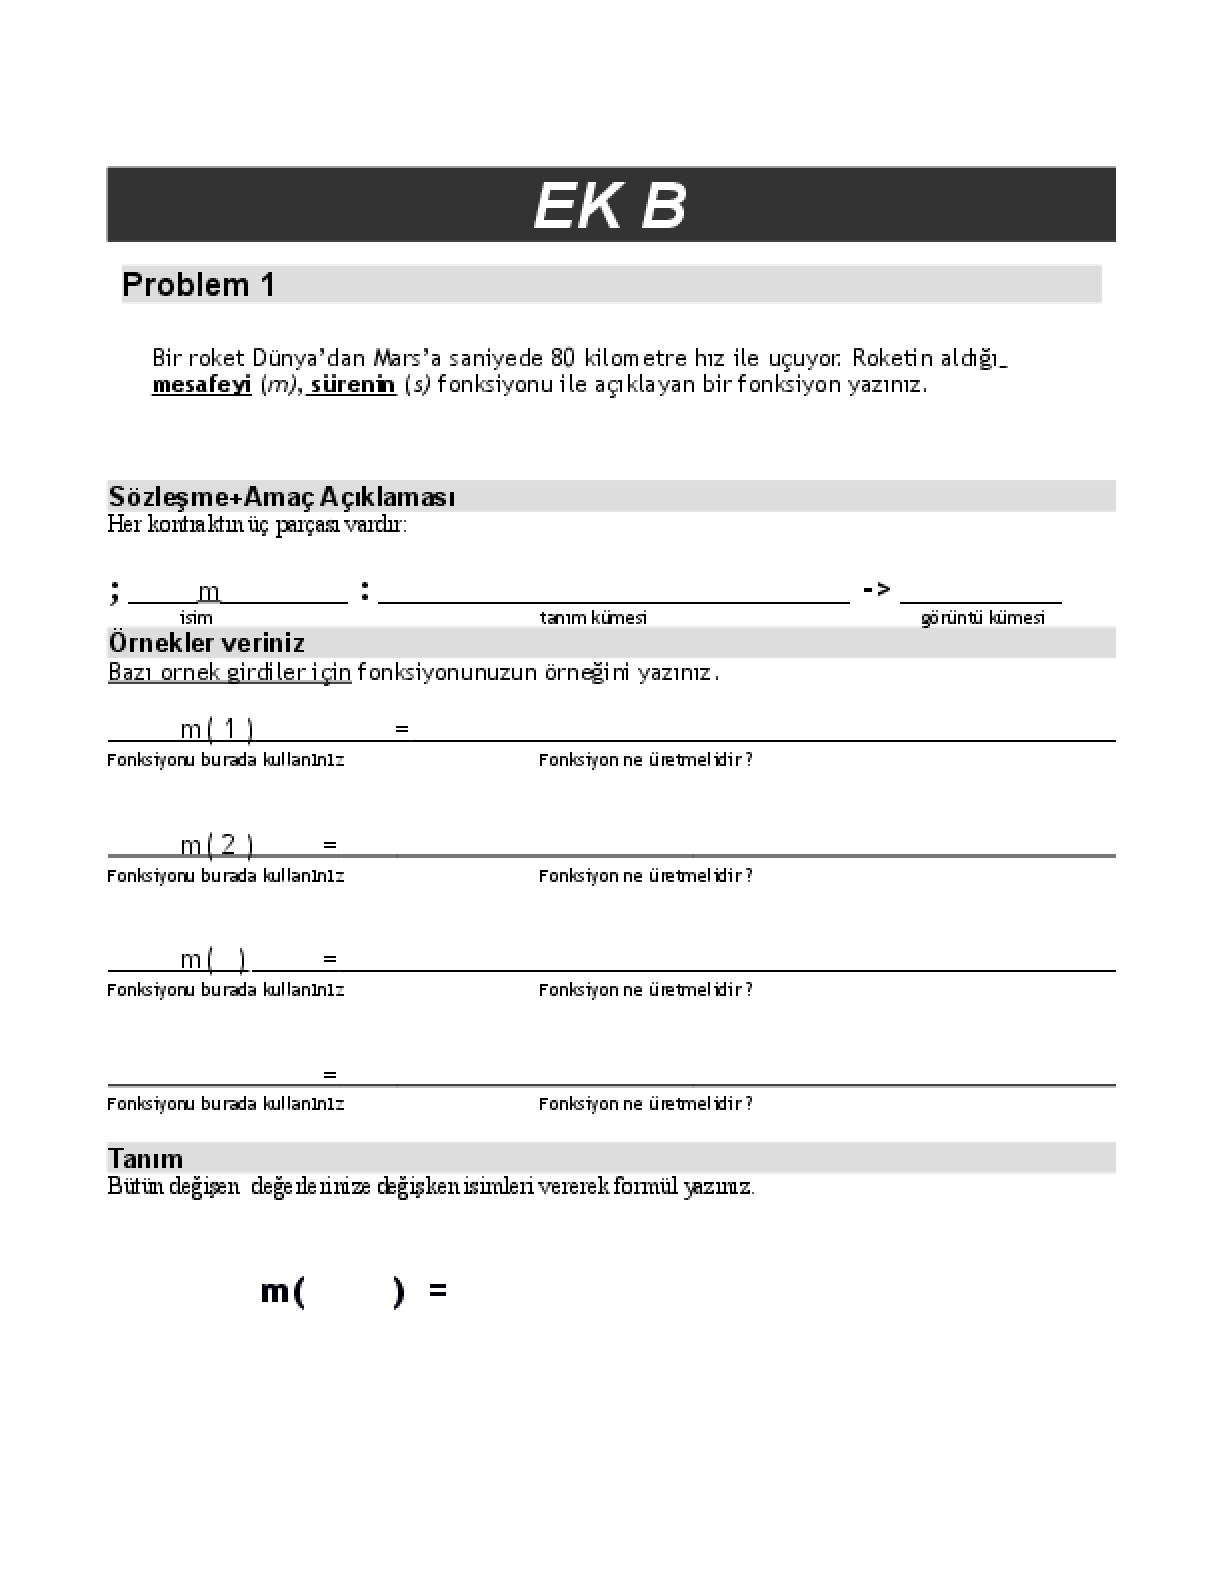
\includegraphics[width=1\linewidth]{cebirsplit-47.png}
\newpage
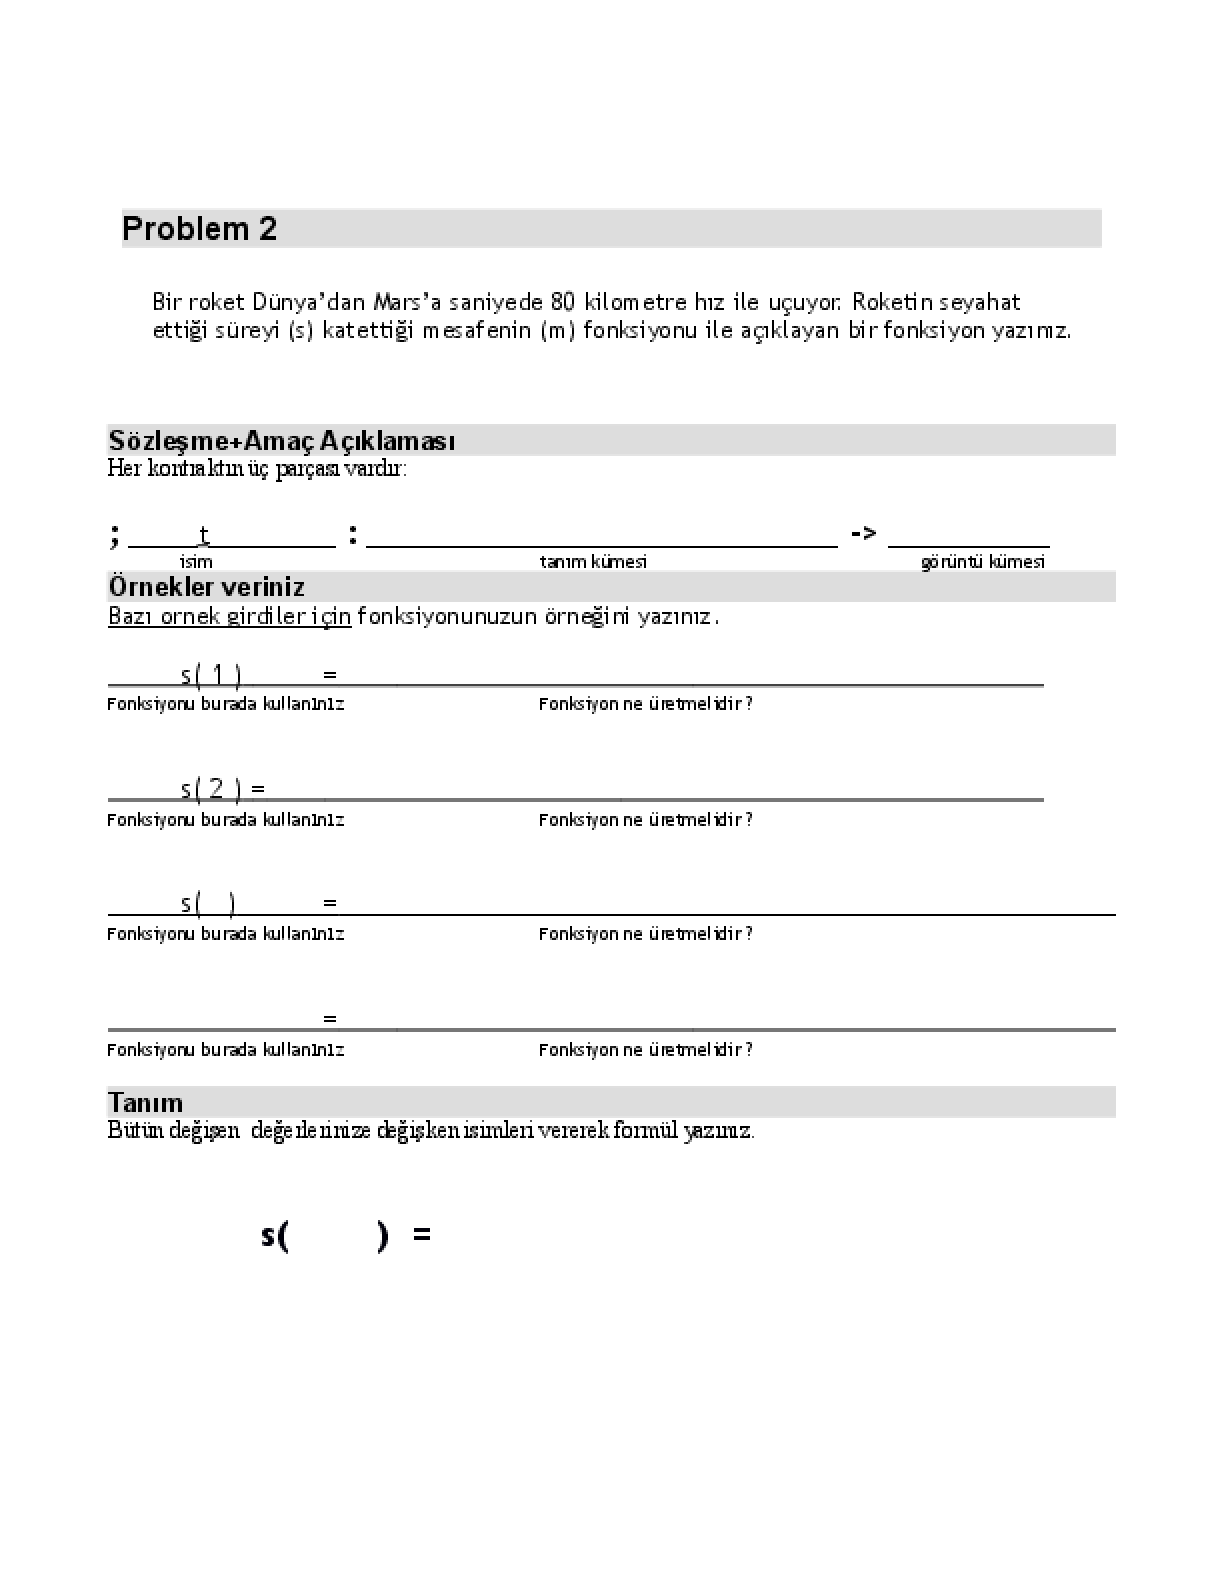
\includegraphics[width=1\linewidth]{cebirsplit-48.png}
\newpage
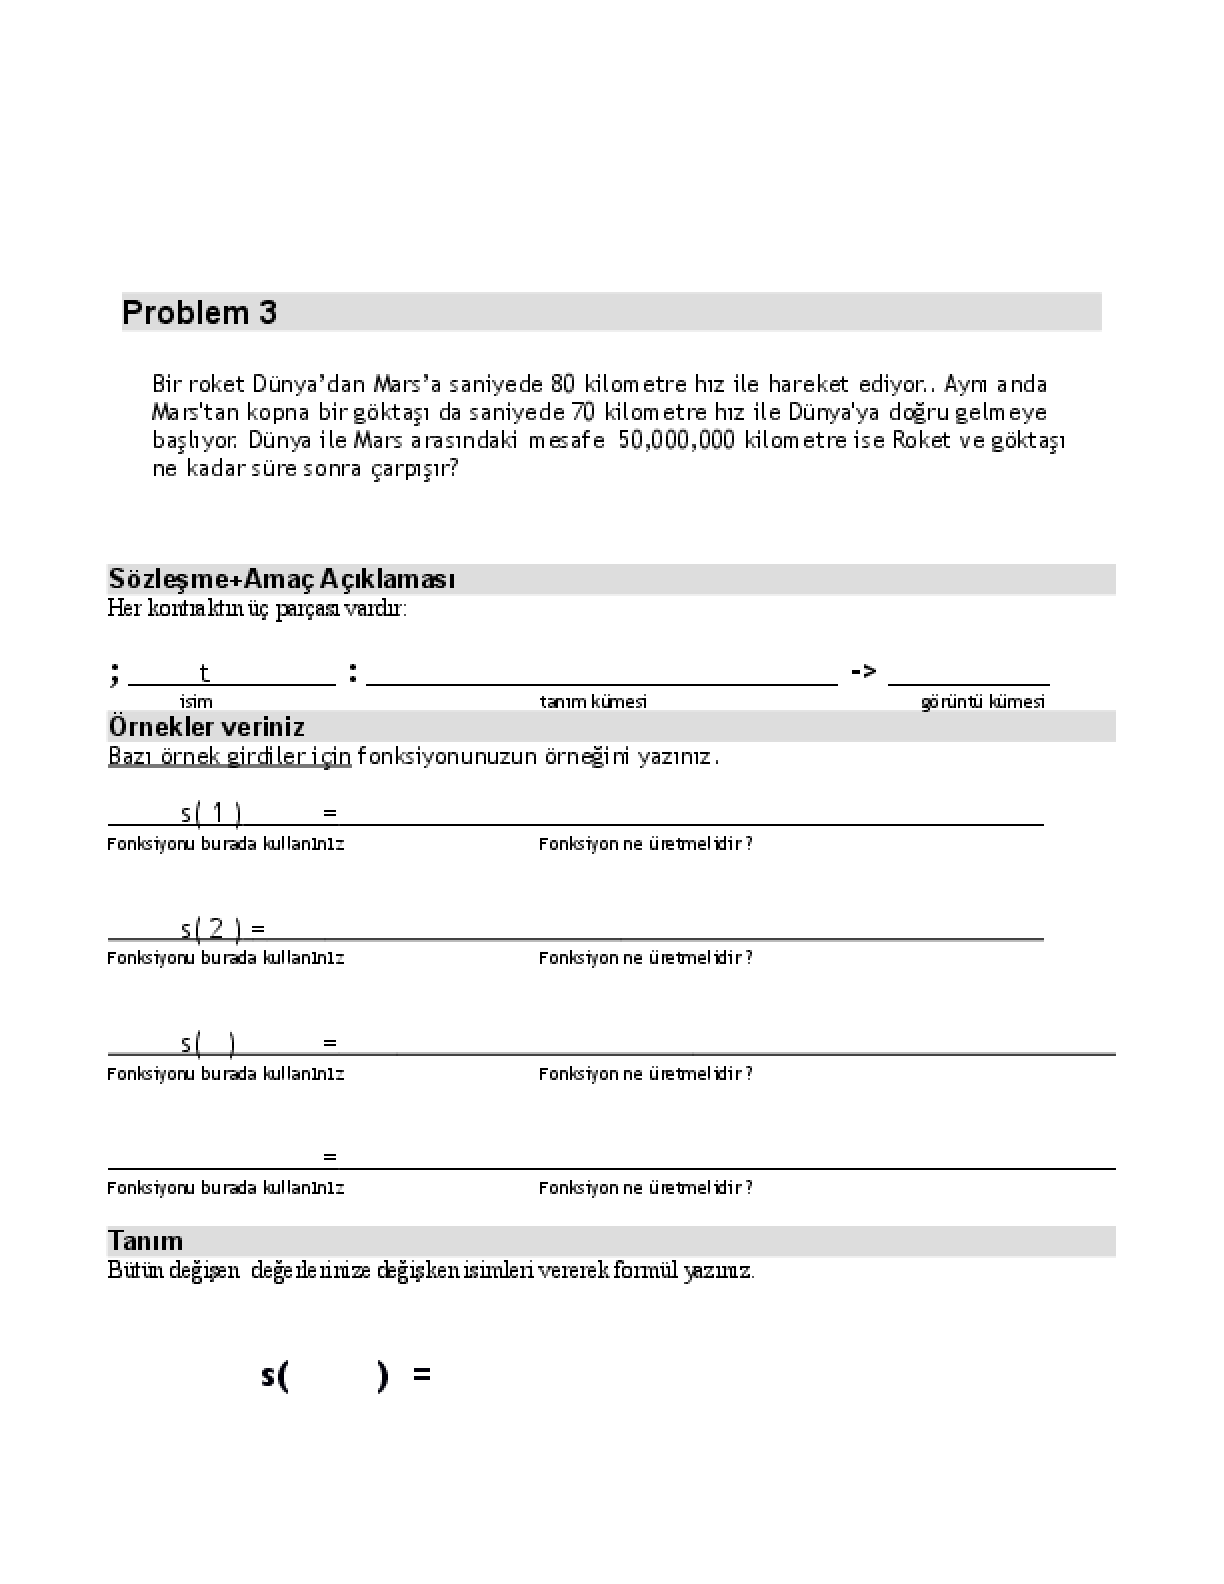
\includegraphics[width=1\linewidth]{cebirsplit-49.png}
\newpage
\includegraphics[width=1\linewidth]{cebirsplit-50.png}
\newpage
\includegraphics[width=1\linewidth]{cebirsplit-51.png}
\newpage
\includegraphics[width=1\linewidth]{cebirsplit-52.png}
\newpage
\includegraphics[width=1\linewidth]{cebirsplit-53.png}
\newpage
\includegraphics[width=1\linewidth]{cebirsplit-54.png}
\newpage
\includegraphics[width=1\linewidth]{cebirsplit-55.png}
\newpage

%\noindent {\large \bf Ad/Soyadı3: \dotfill}\\
\vspace*{0.8cm}
\begin{center}
\includegraphics[width=0.8\linewidth]{reactive.png}

\includegraphics[width=0.25\linewidth]{bootstrap-logo.png}
 
\end{center}

\vspace*{0.2cm}


\begin{center}
{\Large \bf{Nesin Köyleri Cebir ve Programlama Yazokulu 2024 - Evren}}

{\tiny Bootstrap is licensed under a Creative Commons 3.0 Unported License. Based on a work from
www.BootstrapWorld.org. Permissions beyond the scope of this license may be available at
contact@BootstrapWorld.org.

Türkçe versiyonu. Mehmet Gençer, Chris Stephenson ve diğer Nesin Köyleri Cebir ve Programlama Yazokulu öğretim takım üyeleri.

Lisans: Creative Commons 3.0 Unported License} 
\end{center}


\newpage

\subsection*{Veri Yapı Tasarımı}
İsim \fillin[5cm]pasta\\
\vspace{0.5cm}\\
\begin{tabular}{| p{4cm} | p{4cm} | p{8cm} |  }
\hline			
Komponent ismi&Komponent veri tipi&Anlam\\
\hline
renk&color &pastanın rengi \\[10ex]
\hline  
mesaj-rengi&color &mesajın rengi \\[10ex]
\hline  
kat&sayı &pasta katların sayısı \\[10ex]
\hline  
mesaj&metin &pasta üstündeki mesaj \\[10ex]
\hline  
yarı-çap&sayı &pastanın yarı çapı \\[10ex]
\hline  
\end{tabular}

\subsubsection*{Tanım}
\begin{tabular}{| p{17cm} |  }
\hline			
\vspace{0.5cm}
(STRUCT \fillin[3cm]pasta (\fillin[1cm]renk kat mesaj mesaj-rengi yarı-çap ))\\[10ex]
\hline
\end{tabular}





\newpage
\subsection*{Tasarım Recetesi}
\subsubsection*{Sözleşme}
\begin{tabular}{| p{4cm} | p{8cm} | p{4cm} |  }
\hline			
Fonksiyon ismi&Giriş veri tip(ler)i&Sonuç veri tipi\\
\hline
isim-ekle& & \\[10ex]
\hline  
\end{tabular}

\subsubsection*{Amaç}
\begin{tabular}{| p{17cm} |  }
\hline			
Amaç\\
\hline
 \\[10ex]
\hline  
\end{tabular}

\subsubsection*{Örnekler}
\begin{tabular}{| p{4cm} | p{8cm} | p{4cm} |  }
\hline			
Fonksiyon ismi&Giriş veri(ler)i&Sonuç veri\\
\hline
& & \\[6ex]
\hline  
& & \\[6ex]
\hline  
& & \\[6ex]
\hline  
& & \\[6ex]
\hline  
\end{tabular}

\subsubsection*{Şablon}
\begin{tabular}{| p{17cm} |  }
\hline			
Şablon\\
\hline
\vspace{0,2cm}
(define (\fillin[2cm] \hspace{1cm}  \fillin[8cm] ) \\[30ex]
\hline  
\end{tabular}

\newpage
\subsection*{Tasarım Recetesi}
\subsubsection*{Sözleşme}
\begin{tabular}{| p{4cm} | p{8cm} | p{4cm} |  }
\hline			
Fonksiyon ismi&Giriş veri tip(ler)i&Sonuç veri tipi\\
\hline
scale-pasta& & \\[10ex]
\hline  
\end{tabular}

\subsubsection*{Amaç}
\begin{tabular}{| p{17cm} |  }
\hline			
Amaç\\
\hline
 \\[10ex]
\hline  
\end{tabular}

\subsubsection*{Örnekler}
\begin{tabular}{| p{4cm} | p{8cm} | p{4cm} |  }
\hline			
Fonksiyon ismi&Giriş veri(ler)i&Sonuç veri\\
\hline
& & \\[6ex]
\hline  
& & \\[6ex]
\hline  
& & \\[6ex]
\hline  
& & \\[6ex]
\hline  
\end{tabular}

\subsubsection*{Şablon}
\begin{tabular}{| p{17cm} |  }
\hline			
Şablon\\
\hline
\vspace{0,5cm}
\vspace{0,2cm}
(define (\fillin[2cm] \hspace{1cm}  \fillin[8cm] ) \\[30ex]
\hline  
\end{tabular}

\newpage
\subsection*{Tasarım Recetesi}
\subsubsection*{Sözleşme}
\begin{tabular}{| p{4cm} | p{8cm} | p{4cm} |  }
\hline			
Fonksiyon ismi&Giriş veri tip(ler)i&Sonuç veri tipi\\
\hline
çift-kat& & \\[10ex]
\hline  
\end{tabular}

\subsubsection*{Amaç}
\begin{tabular}{| p{17cm} |  }
\hline			
Amaç\\
\hline
 \\[10ex]
\hline  
\end{tabular}

\subsubsection*{Örnekler}
\begin{tabular}{| p{4cm} | p{8cm} | p{4cm} |  }
\hline			
Fonksiyon ismi&Giriş veri(ler)i&Sonuç veri\\
\hline
& & \\[6ex]
\hline  
& & \\[6ex]
\hline  
& & \\[6ex]
\hline  
& & \\[6ex]
\hline  
\end{tabular}

\subsubsection*{Şablon}
\begin{tabular}{| p{17cm} |  }
\hline			
Şablon\\
\hline
\vspace{0,5cm}
\vspace{0,2cm}
(define (\fillin[2cm] \hspace{1cm}  \fillin[8cm] ) \\[30ex]
\hline  
\end{tabular}



%%%%%%%%%%%%%%%%%%%%%%%%%%%%%%%%%%%%%%
%           Veri Yapı
%%%%%%%%%%%%%%%%%%%%%%%%%%%%%%%%%%%%%%
\newpage
\subsection*{Veri Yapı Tasarımı}
İsim v\\
\vspace{0.5cm}\\
\begin{tabular}{| p{4cm} | p{4cm} | p{8cm} |  }
\hline			
Komponent ismi&Komponent veri tipi&Anlam\\
\hline
& & \\[10ex]
\hline  
& & \\[10ex]
\hline  
\end{tabular}

\subsubsection*{Tanım}
\begin{tabular}{| p{17cm} |  }
\hline			
\vspace{0.5cm}
(STRUCT \fillin[3cm] (\fillin[10cm] ))\\[10ex]
\hline
\end{tabular}


%%%%%%%%%%%%%%%%%%%%%%%%%%%%%%%%%%%%%%
%           Veri Yapı Son
%%%%%%%%%%%%%%%%%%%%%%%%%%%%%%%%%%%%%%




%%%%%%%%%%%%%%%%%%%%%%%%%%%%%%%%%%%%
%   Tasarım Recetesi
%%%%%%%%%%%%%%%%%%%%%%%%%%%%%%%%%%%%
\newpage
\subsection*{Tasarım Recetesi}
\subsubsection*{Sözleşme}
\begin{tabular}{| p{4cm} | p{8cm} | p{4cm} |  }
\hline			
Fonksiyon ismi&Giriş veri tip(ler)i&Sonuç veri tipi\\
\hline
v+& & \\[10ex]
\hline  
\end{tabular}

\subsubsection*{Amaç}
\begin{tabular}{| p{17cm} |  }
\hline			
Amaç\\
\hline
 \\[10ex]
\hline  
\end{tabular}

\subsubsection*{Örnekler}
\begin{tabular}{| p{4cm} | p{8cm} | p{4cm} |  }
\hline			
Fonksiyon ismi&Giriş veri(ler)i&Sonuç veri\\
\hline
& & \\[6ex]
\hline  
& & \\[6ex]
\hline  
& & \\[6ex]
\hline  
& & \\[6ex]
\hline  
\end{tabular}

\subsubsection*{Şablon}
\begin{tabular}{| p{17cm} |  }
\hline			
Şablon\\
\hline
\vspace{0,5cm}
\vspace{0,2cm}
(define (\fillin[2cm] \hspace{1cm}  \fillin[8cm] ) \\[30ex]
\hline  
\end{tabular}


%%%%%%%%%%%%%%%%%%%%%%%%%%%%%%%%%%%%
%   Tasarım Recetesi Son
%%%%%%%%%%%%%%%%%%%%%%%%%%%%%%%%%%%%




%%%%%%%%%%%%%%%%%%%%%%%%%%%%%%%%%%%%
%   Tasarım Recetesi
%%%%%%%%%%%%%%%%%%%%%%%%%%%%%%%%%%%%
\newpage
\subsection*{Tasarım Recetesi}
\subsubsection*{Sözleşme}
\begin{tabular}{| p{4cm} | p{8cm} | p{4cm} |  }
\hline			
Fonksiyon ismi&Giriş veri tip(ler)i&Sonuç veri tipi\\
\hline
v-& & \\[10ex]
\hline  
\end{tabular}

\subsubsection*{Amaç}
\begin{tabular}{| p{17cm} |  }
\hline			
Amaç\\
\hline
 \\[10ex]
\hline  
\end{tabular}

\subsubsection*{Örnekler}
\begin{tabular}{| p{4cm} | p{8cm} | p{4cm} |  }
\hline			
Fonksiyon ismi&Giriş veri(ler)i&Sonuç veri\\
\hline
& & \\[6ex]
\hline  
& & \\[6ex]
\hline  
& & \\[6ex]
\hline  
& & \\[6ex]
\hline  
\end{tabular}

\subsubsection*{Şablon}
\begin{tabular}{| p{17cm} |  }
\hline			
Şablon\\
\hline
\vspace{0,5cm}
\vspace{0,2cm}
(define (\fillin[2cm] \hspace{1cm}  \fillin[8cm] ) \\[30ex]
\hline  
\end{tabular}


%%%%%%%%%%%%%%%%%%%%%%%%%%%%%%%%%%%%
%   Tasarım Recetesi Son
%%%%%%%%%%%%%%%%%%%%%%%%%%%%%%%%%%%%




%%%%%%%%%%%%%%%%%%%%%%%%%%%%%%%%%%%%
%   Tasarım Recetesi
%%%%%%%%%%%%%%%%%%%%%%%%%%%%%%%%%%%%
\newpage
\subsection*{Tasarım Recetesi}
\subsubsection*{Sözleşme}
\begin{tabular}{| p{4cm} | p{8cm} | p{4cm} |  }
\hline			
Fonksiyon ismi&Giriş veri tip(ler)i&Sonuç veri tipi\\
\hline
v.& & \\[10ex]
\hline  
\end{tabular}

\subsubsection*{Amaç}
\begin{tabular}{| p{17cm} |  }
\hline			
Amaç\\
\hline
 \\[10ex]
\hline  
\end{tabular}

\subsubsection*{Örnekler}
\begin{tabular}{| p{4cm} | p{8cm} | p{4cm} |  }
\hline			
Fonksiyon ismi&Giriş veri(ler)i&Sonuç veri\\
\hline
& & \\[6ex]
\hline  
& & \\[6ex]
\hline  
& & \\[6ex]
\hline  
& & \\[6ex]
\hline  
\end{tabular}

\subsubsection*{Şablon}
\begin{tabular}{| p{17cm} |  }
\hline			
Şablon\\
\hline
\vspace{0,5cm}
\vspace{0,2cm}
(define (\fillin[2cm] \hspace{1cm}  \fillin[8cm] ) \\[30ex]
\hline  
\end{tabular}


%%%%%%%%%%%%%%%%%%%%%%%%%%%%%%%%%%%%
%   Tasarım Recetesi Son
%%%%%%%%%%%%%%%%%%%%%%%%%%%%%%%%%%%%




%%%%%%%%%%%%%%%%%%%%%%%%%%%%%%%%%%%%
%   Tasarım Recetesi
%%%%%%%%%%%%%%%%%%%%%%%%%%%%%%%%%%%%
\newpage
\subsection*{Tasarım Recetesi}
\subsubsection*{Sözleşme}
\begin{tabular}{| p{4cm} | p{8cm} | p{4cm} |  }
\hline			
Fonksiyon ismi&Giriş veri tip(ler)i&Sonuç veri tipi\\
\hline
v*& & \\[10ex]
\hline  
\end{tabular}

\subsubsection*{Amaç}
\begin{tabular}{| p{17cm} |  }
\hline			
Amaç\\
\hline
 \\[10ex]
\hline  
\end{tabular}

\subsubsection*{Örnekler}
\begin{tabular}{| p{4cm} | p{8cm} | p{4cm} |  }
\hline			
Fonksiyon ismi&Giriş veri(ler)i&Sonuç veri\\
\hline
& & \\[6ex]
\hline  
& & \\[6ex]
\hline  
& & \\[6ex]
\hline  
& & \\[6ex]
\hline  
\end{tabular}

\subsubsection*{Şablon}
\begin{tabular}{| p{17cm} |  }
\hline			
Şablon\\
\hline
\vspace{0,5cm}
\vspace{0,2cm}
(define (\fillin[2cm] \hspace{1cm}  \fillin[8cm] ) \\[30ex]
\hline  
\end{tabular}


%%%%%%%%%%%%%%%%%%%%%%%%%%%%%%%%%%%%
%   Tasarım Recetesi Son
%%%%%%%%%%%%%%%%%%%%%%%%%%%%%%%%%%%%




%%%%%%%%%%%%%%%%%%%%%%%%%%%%%%%%%%%%
%   Tasarım Recetesi
%%%%%%%%%%%%%%%%%%%%%%%%%%%%%%%%%%%%
\newpage
\subsection*{Tasarım Recetesi}
\subsubsection*{Sözleşme}
\begin{tabular}{| p{4cm} | p{8cm} | p{4cm} |  }
\hline			
Fonksiyon ismi&Giriş veri tip(ler)i&Sonuç veri tipi\\
\hline
v-mag& & \\[10ex]
\hline  
\end{tabular}

\subsubsection*{Amaç}
\begin{tabular}{| p{17cm} |  }
\hline			
Amaç\\
\hline
 \\[10ex]
\hline  
\end{tabular}

\subsubsection*{Örnekler}
\begin{tabular}{| p{4cm} | p{8cm} | p{4cm} |  }
\hline			
Fonksiyon ismi&Giriş veri(ler)i&Sonuç veri\\
\hline
& & \\[6ex]
\hline  
& & \\[6ex]
\hline  
& & \\[6ex]
\hline  
& & \\[6ex]
\hline  
\end{tabular}

\subsubsection*{Şablon}
\begin{tabular}{| p{17cm} |  }
\hline			
Şablon\\
\hline
\vspace{0,2cm}
(define (\fillin[2cm] \hspace{1cm}  \fillin[8cm] ) \\[30ex]
\hline  
\end{tabular}


%%%%%%%%%%%%%%%%%%%%%%%%%%%%%%%%%%%%
%   Tasarım Recetesi Son
%%%%%%%%%%%%%%%%%%%%%%%%%%%%%%%%%%%%

\newpage
\section*{Oyun Hikayesi}
 
\noindent
\begin{tabular}{| p{16.5cm}  |  }
\hline			
Sahne 1\\
\hline
 \\[50ex]
\hline  
\end{tabular}

\vspace{5ex}
\noindent
\begin{tabular}{| p{16.5cm}  |  }
\hline			
Sahne 2\\
\hline
 \\[50ex]
\hline  
\end{tabular}

\vspace{5ex}
\noindent
\begin{tabular}{| p{16.5cm}  |  }
\hline			
Sahne 3\\
\hline
 \\[50ex]
\hline  
\end{tabular}

\vspace{5ex}
\noindent
\begin{tabular}{| p{16.5cm}  |  }
\hline			
Sahne 4\\
\hline
 \\[50ex]
\hline  
\end{tabular}

\vspace{5ex}
\noindent
\begin{tabular}{| p{16.5cm}  |  }
\hline			
Sahne 5\\
\hline
 \\[50ex]
\hline  
\end{tabular}

\vspace{5ex}

\subsubsection*{Neler değişiyor?}
\begin{tabular}{| p{4cm} | p{11cm} |  }
\hline			
Nesne&Nasıl değişir?\\
\hline
& \\[6ex]
\hline  
& \\[6ex]
\hline  
& \\[6ex]
\hline  
& \\[6ex]
\hline  
& \\[6ex]
\hline  
\end{tabular}


\subsubsection*{Neler değişiyor?}
\begin{tabular}{| p{4cm} | p{11cm} |  }
\hline			
Nesne&Nasıl değişir?\\
\hline
& \\[6ex]
\hline  
& \\[6ex]
\hline  
& \\[6ex]
\hline  
& \\[6ex]
\hline  
& \\[6ex]
\hline  
\end{tabular}


\subsubsection*{Veriler}
\begin{tabular}{| p{4cm} | p{11cm} |  }
\hline			
Veri ismi&Veri tipi\\
\hline
& \\[2ex]
\hline  
& \\[2ex]
\hline  
& \\[2ex]
\hline  
& \\[2ex]
\hline  
& \\[2ex]
\hline  
& \\[2ex]
\hline  
& \\[2ex]
\hline  
& \\[2ex]
\hline  
& \\[2ex]
\hline  
& \\[2ex]
\hline  
& \\[2ex]
\hline  
& \\[2ex]
\hline  
& \\[2ex]
\hline  
& \\[2ex]
\hline  
& \\[2ex]
\hline  
& \\[2ex]
\hline  
& \\[2ex]
\hline  
& \\[2ex]
\hline  
\end{tabular}



%%%%%%%%%%%%%%%%%%%%%%%%%%%%%%%%%%%%%%
%           Veri Yapı
%%%%%%%%%%%%%%%%%%%%%%%%%%%%%%%%%%%%%%
\newpage
\subsection*{Veri Yapı Tasarımı}
İsim  \fillin[5cm]\\
\vspace{0.5cm}\\
\begin{tabular}{| p{4cm} | p{4cm} | p{8cm} |  }
\hline			
Komponent ismi&Komponent veri tipi&Anlam\\
\hline
& & \\[10ex]
\hline  
& & \\[10ex]
\hline  
& & \\[10ex]
\hline  
& & \\[10ex]
\hline  
& & \\[10ex]
\hline  
& & \\[10ex]
\hline  
& & \\[10ex]
\hline  
\end{tabular}

\subsubsection*{Tanım}
\begin{tabular}{| p{17cm} |  }
\hline			
\vspace{0.5cm}
(STRUCT \fillin[3cm] (\fillin[10cm] ))\\[10ex]
\hline
\end{tabular}


%%%%%%%%%%%%%%%%%%%%%%%%%%%%%%%%%%%%%%
%           Veri Yapı Son
%%%%%%%%%%%%%%%%%%%%%%%%%%%%%%%%%%%%%%




%%%%%%%%%%%%%%%%%%%%%%%%%%%%%%%%%%%%
%   Tasarım Recetesi
%%%%%%%%%%%%%%%%%%%%%%%%%%%%%%%%%%%%
\newpage
\subsection*{Tasarım Recetesi}
\subsubsection*{Sözleşme}
\begin{tabular}{| p{4cm} | p{8cm} | p{4cm} |  }
\hline			
Fonksiyon ismi&Giriş veri tip(ler)i&Sonuç veri tipi\\
\hline
nesne-çiz& & \\[10ex]
\hline  
\end{tabular}

\subsubsection*{Amaç}
\begin{tabular}{| p{17cm} |  }
\hline			
Amaç\\
\hline
 \\[10ex]
\hline  
\end{tabular}

\subsubsection*{Örnekler}
\begin{tabular}{| p{4cm} | p{8cm} | p{4cm} |  }
\hline			
Fonksiyon ismi&Giriş veri(ler)i&Sonuç veri\\
\hline
& & \\[6ex]
\hline  
& & \\[6ex]
\hline  
& & \\[6ex]
\hline  
& & \\[6ex]
\hline  
\end{tabular}

\subsubsection*{Şablon}
\begin{tabular}{| p{17cm} |  }
\hline			
Şablon\\
\hline
\vspace{0,2cm}
(define (\fillin[2cm] \hspace{1cm}  \fillin[8cm] ) \\[30ex]
\hline  
\end{tabular}


%%%%%%%%%%%%%%%%%%%%%%%%%%%%%%%%%%%%
%   Tasarım Recetesi Son
%%%%%%%%%%%%%%%%%%%%%%%%%%%%%%%%%%%%



%%%%%%%%%%%%%%%%%%%%%%%%%%%%%%%%%%%%
%   Tasarım Recetesi
%%%%%%%%%%%%%%%%%%%%%%%%%%%%%%%%%%%%
\newpage
\subsection*{Tasarım Recetesi}
\subsubsection*{Sözleşme}
\begin{tabular}{| p{4cm} | p{8cm} | p{4cm} |  }
\hline			
Fonksiyon ismi&Giriş veri tip(ler)i&Sonuç veri tipi\\
\hline
nesne-fizik-güncelle& & \\[10ex]
\hline  
\end{tabular}

\subsubsection*{Amaç}
\begin{tabular}{| p{17cm} |  }
\hline			
Amaç\\
\hline
 \\[10ex]
\hline  
\end{tabular}

\subsubsection*{Örnekler}
\begin{tabular}{| p{4cm} | p{8cm} | p{4cm} |  }
\hline			
Fonksiyon ismi&Giriş veri(ler)i&Sonuç veri\\
\hline
& & \\[6ex]
\hline  
& & \\[6ex]
\hline  
& & \\[6ex]
\hline  
& & \\[6ex]
\hline  
\end{tabular}

\subsubsection*{Şablon}
\begin{tabular}{| p{17cm} |  }
\hline			
Şablon\\
\hline
\vspace{0,2cm}
(define (\fillin[2cm] \hspace{1cm}  \fillin[8cm] ) \\[30ex]
\hline  
\end{tabular}


%%%%%%%%%%%%%%%%%%%%%%%%%%%%%%%%%%%%
%   Tasarım Recetesi Son
%%%%%%%%%%%%%%%%%%%%%%%%%%%%%%%%%%%%




%%%%%%%%%%%%%%%%%%%%%%%%%%%%%%%%%%%%%%
%           Veri Yapı
%%%%%%%%%%%%%%%%%%%%%%%%%%%%%%%%%%%%%%
\newpage
\subsection*{Veri Yapı Tasarımı}
İsim evren\\
\vspace{0.5cm}\\
\begin{tabular}{| p{4cm} | p{4cm} | p{8cm} |  }
\hline			
Komponent ismi&Komponent veri tipi&Anlam\\
\hline
& & \\[10ex]
\hline  
& & \\[10ex]
\hline  
& & \\[10ex]
\hline  
& & \\[10ex]
\hline  
& & \\[10ex]
\hline  
& & \\[10ex]
\hline  
& & \\[10ex]
\hline  
\end{tabular}

\subsubsection*{Tanım}
\begin{tabular}{| p{17cm} |  }
\hline			
\vspace{0.5cm}
(STRUCT \fillin[3cm] (\fillin[10cm] ))\\[10ex]
\hline
\end{tabular}


%%%%%%%%%%%%%%%%%%%%%%%%%%%%%%%%%%%%%%
%           Veri Yapı Son
%%%%%%%%%%%%%%%%%%%%%%%%%%%%%%%%%%%%%%





%%%%%%%%%%%%%%%%%%%%%%%%%%%%%%%%%%%%
%   Tasarım Recetesi
%%%%%%%%%%%%%%%%%%%%%%%%%%%%%%%%%%%%
\newpage
\subsection*{Tasarım Recetesi}
\subsubsection*{Sözleşme}
\begin{tabular}{| p{4cm} | p{8cm} | p{4cm} |  }
\hline			
Fonksiyon ismi&Giriş veri tip(ler)i&Sonuç veri tipi\\
\hline
evren-çiz& & \\[10ex]
\hline  
\end{tabular}

\subsubsection*{Amaç}
\begin{tabular}{| p{17cm} |  }
\hline			
Amaç\\
\hline
 \\[10ex]
\hline  
\end{tabular}

\subsubsection*{Örnekler}
\begin{tabular}{| p{4cm} | p{8cm} | p{4cm} |  }
\hline			
Fonksiyon ismi&Giriş veri(ler)i&Sonuç veri\\
\hline
& & \\[6ex]
\hline  
& & \\[6ex]
\hline  
& & \\[6ex]
\hline  
& & \\[6ex]
\hline  
\end{tabular}

\subsubsection*{Şablon}
\begin{tabular}{| p{17cm} |  }
\hline			
Şablon\\
\hline
\vspace{0,2cm}
(define (\fillin[2cm] \hspace{1cm}  \fillin[8cm] ) \\[30ex]
\hline  
\end{tabular}


%%%%%%%%%%%%%%%%%%%%%%%%%%%%%%%%%%%%
%   Tasarım Recetesi Son
%%%%%%%%%%%%%%%%%%%%%%%%%%%%%%%%%%%%




%%%%%%%%%%%%%%%%%%%%%%%%%%%%%%%%%%%%
%   Tasarım Recetesi
%%%%%%%%%%%%%%%%%%%%%%%%%%%%%%%%%%%%
\newpage
\subsection*{Tasarım Recetesi}
\subsubsection*{Sözleşme}
\begin{tabular}{| p{4cm} | p{8cm} | p{4cm} |  }
\hline			
Fonksiyon ismi&Giriş veri tip(ler)i&Sonuç veri tipi\\
\hline
evren-güncelle& & \\[10ex]
\hline  
\end{tabular}

\subsubsection*{Amaç}
\begin{tabular}{| p{17cm} |  }
\hline			
Amaç\\
\hline
 \\[10ex]
\hline  
\end{tabular}

\subsubsection*{Örnekler}
\begin{tabular}{| p{4cm} | p{8cm} | p{4cm} |  }
\hline			
Fonksiyon ismi&Giriş veri(ler)i&Sonuç veri\\
\hline
& & \\[6ex]
\hline  
& & \\[6ex]
\hline  
& & \\[6ex]
\hline  
& & \\[6ex]
\hline  
\end{tabular}

\subsubsection*{Şablon}
\begin{tabular}{| p{17cm} |  }
\hline			
Şablon\\
\hline
\vspace{0,2cm}
(define (\fillin[2cm] \hspace{1cm}  \fillin[8cm] ) \\[30ex]
\hline  
\end{tabular}
%%%%%%%%%%%%%%%%%%%%%%%%%%%%%%%%%%%%
%   Tasarım Recetesi Son
%%%%%%%%%%%%%%%%%%%%%%%%%%%%%%%%%%%%





%%%%%%%%%%%%%%%%%%%%%%%%%%%%%%%%%%%%
%   Tasarım Recetesi
%%%%%%%%%%%%%%%%%%%%%%%%%%%%%%%%%%%%
\newpage
\subsection*{Tasarım Recetesi}
\subsubsection*{Sözleşme}
\begin{tabular}{| p{4cm} | p{8cm} | p{4cm} |  }
\hline			
Fonksiyon ismi&Giriş veri tip(ler)i&Sonuç veri tipi\\
\hline
alttan-sek& & \\[10ex]
\hline  
\end{tabular}

\subsubsection*{Amaç}
\begin{tabular}{| p{17cm} |  }
\hline			
Amaç\\
\hline
 \\[10ex]
\hline  
\end{tabular}

\subsubsection*{Örnekler}
\begin{tabular}{| p{4cm} | p{8cm} | p{4cm} |  }
\hline			
Fonksiyon ismi&Giriş veri(ler)i&Sonuç veri\\
\hline
& & \\[6ex]
\hline  
& & \\[6ex]
\hline  
& & \\[6ex]
\hline  
& & \\[6ex]
\hline  
\end{tabular}

\subsubsection*{Şablon}
\begin{tabular}{| p{17cm} |  }
\hline			
Şablon\\
\hline
\vspace{0,2cm}
(define (\fillin[2cm] \hspace{1cm}  \fillin[8cm] ) \\[30ex]
\hline  
\end{tabular}
%%%%%%%%%%%%%%%%%%%%%%%%%%%%%%%%%%%%
%   Tasarım Recetesi Son
%%%%%%%%%%%%%%%%%%%%%%%%%%%%%%%%%%%%


\section*{Benin Oyunumun Hikayesi}

\noindent
\begin{tabular}{| p{16.5cm}  |  }
\hline			
Sahne 1\\
\hline
 \\[50ex]
\hline  
\end{tabular}

\vspace{5ex}
\noindent
\begin{tabular}{| p{16.5cm}  |  }
\hline			
Sahne 2\\
\hline
 \\[50ex]
\hline  
\end{tabular}

\vspace{5ex}
\noindent
\begin{tabular}{| p{16.5cm}  |  }
\hline			
Sahne 3\\
\hline
 \\[50ex]
\hline  
\end{tabular}

\vspace{5ex}
\noindent
\begin{tabular}{| p{16.5cm}  |  }
\hline			
Sahne 4\\
\hline
 \\[50ex]
\hline  
\end{tabular}

\vspace{5ex}
\noindent
\begin{tabular}{| p{16.5cm}  |  }
\hline			
Sahne 5\\
\hline
 \\[50ex]
\hline  
\end{tabular}

\subsubsection*{Neler değişiyor?}
\begin{tabular}{| p{4cm} | p{11cm} |  }
\hline			
Nesne&Nasıl değişir?\\
\hline
& \\[6ex]
\hline  
& \\[6ex]
\hline  
& \\[6ex]
\hline  
& \\[6ex]
\hline  
& \\[6ex]
\hline  
\end{tabular}


\subsubsection*{Veri yapılar}
\begin{tabular}{| p{4cm} | p{11cm} |  }
\hline			
Veri yapı ismi&Veri tipi\\
\hline
& \\[2ex]
\hline  
& \\[2ex]
\hline  
& \\[2ex]
\hline  
& \\[2ex]
\hline  
& \\[2ex]
\hline  
& \\[2ex]
\hline  
& \\[2ex]
\hline  
& \\[2ex]
\hline  
& \\[2ex]
\hline  
& \\[2ex]
\hline  
& \\[2ex]
\hline  
& \\[2ex]
\hline  
& \\[2ex]
\hline  
& \\[2ex]
\hline  
& \\[2ex]
\hline  
& \\[2ex]
\hline  
& \\[2ex]
\hline  
& \\[2ex]
\hline  
\end{tabular}




%%%%%%%%%%%%%%%%%%%%%%%%%%%%%%%%%%%%%%
%           Veri Yapı
%%%%%%%%%%%%%%%%%%%%%%%%%%%%%%%%%%%%%%
\newpage
\subsection*{Veri Yapı Tasarımı}
İsim  \fillin[5cm]\\
\vspace{0.5cm}\\
\begin{tabular}{| p{4cm} | p{4cm} | p{8cm} |  }
\hline			
Komponent ismi&Komponent veri tipi&Anlam\\
\hline
& & \\[10ex]
\hline  
& & \\[10ex]
\hline  
& & \\[10ex]
\hline  
& & \\[10ex]
\hline  
& & \\[10ex]
\hline  
& & \\[10ex]
\hline  
& & \\[10ex]
\hline  
\end{tabular}

\subsubsection*{Tanım}
\begin{tabular}{| p{17cm} |  }
\hline			
\vspace{0.5cm}
(STRUCT \fillin[3cm] (\fillin[10cm] ))\\[10ex]
\hline
\end{tabular}


%%%%%%%%%%%%%%%%%%%%%%%%%%%%%%%%%%%%%%
%           Veri Yapı Son
%%%%%%%%%%%%%%%%%%%%%%%%%%%%%%%%%%%%%%



%%%%%%%%%%%%%%%%%%%%%%%%%%%%%%%%%%%%%%
%           Veri Yapı
%%%%%%%%%%%%%%%%%%%%%%%%%%%%%%%%%%%%%%
\newpage
\subsection*{Veri Yapı Tasarımı}
İsim  \fillin[5cm]\\
\vspace{0.5cm}\\
\begin{tabular}{| p{4cm} | p{4cm} | p{8cm} |  }
\hline			
Komponent ismi&Komponent veri tipi&Anlam\\
\hline
& & \\[10ex]
\hline  
& & \\[10ex]
\hline  
& & \\[10ex]
\hline  
& & \\[10ex]
\hline  
& & \\[10ex]
\hline  
& & \\[10ex]
\hline  
& & \\[10ex]
\hline  
\end{tabular}

\subsubsection*{Tanım}
\begin{tabular}{| p{17cm} |  }
\hline			
\vspace{0.5cm}
(STRUCT \fillin[3cm] (\fillin[10cm] ))\\[10ex]
\hline
\end{tabular}


%%%%%%%%%%%%%%%%%%%%%%%%%%%%%%%%%%%%%%
%           Veri Yapı Son
%%%%%%%%%%%%%%%%%%%%%%%%%%%%%%%%%%%%%%



%%%%%%%%%%%%%%%%%%%%%%%%%%%%%%%%%%%%%%
%           Veri Yapı
%%%%%%%%%%%%%%%%%%%%%%%%%%%%%%%%%%%%%%
\newpage
\subsection*{Veri Yapı Tasarımı}
İsim  \fillin[5cm]\\
\vspace{0.5cm}\\
\begin{tabular}{| p{4cm} | p{4cm} | p{8cm} |  }
\hline			
Komponent ismi&Komponent veri tipi&Anlam\\
\hline
& & \\[10ex]
\hline  
& & \\[10ex]
\hline  
& & \\[10ex]
\hline  
& & \\[10ex]
\hline  
& & \\[10ex]
\hline  
& & \\[10ex]
\hline  
& & \\[10ex]
\hline  
\end{tabular}

\subsubsection*{Tanım}
\begin{tabular}{| p{17cm} |  }
\hline			
\vspace{0.5cm}
(STRUCT \fillin[3cm] (\fillin[10cm] ))\\[10ex]
\hline
\end{tabular}


%%%%%%%%%%%%%%%%%%%%%%%%%%%%%%%%%%%%%%
%           Veri Yapı Son
%%%%%%%%%%%%%%%%%%%%%%%%%%%%%%%%%%%%%%



%%%%%%%%%%%%%%%%%%%%%%%%%%%%%%%%%%%%%%
%           Veri Yapı
%%%%%%%%%%%%%%%%%%%%%%%%%%%%%%%%%%%%%%
\newpage
\subsection*{Veri Yapı Tasarımı}
İsim  \fillin[5cm]\\
\vspace{0.5cm}\\
\begin{tabular}{| p{4cm} | p{4cm} | p{8cm} |  }
\hline			
Komponent ismi&Komponent veri tipi&Anlam\\
\hline
& & \\[10ex]
\hline  
& & \\[10ex]
\hline  
& & \\[10ex]
\hline  
& & \\[10ex]
\hline  
& & \\[10ex]
\hline  
& & \\[10ex]
\hline  
& & \\[10ex]
\hline  
\end{tabular}

\subsubsection*{Tanım}
\begin{tabular}{| p{17cm} |  }
\hline			
\vspace{0.5cm}
(STRUCT \fillin[3cm] (\fillin[10cm] ))\\[10ex]
\hline
\end{tabular}


%%%%%%%%%%%%%%%%%%%%%%%%%%%%%%%%%%%%%%
%           Veri Yapı Son
%%%%%%%%%%%%%%%%%%%%%%%%%%%%%%%%%%%%%%





%%%%%%%%%%%%%%%%%%%%%%%%%%%%%%%%%%%%%%
%           Veri Yapı
%%%%%%%%%%%%%%%%%%%%%%%%%%%%%%%%%%%%%%
\newpage
\subsection*{Veri Yapı Tasarımı}
İsim  \fillin[5cm]\\
\vspace{0.5cm}\\
\begin{tabular}{| p{4cm} | p{4cm} | p{8cm} |  }
\hline			
Komponent ismi&Komponent veri tipi&Anlam\\
\hline
& & \\[10ex]
\hline  
& & \\[10ex]
\hline  
& & \\[10ex]
\hline  
& & \\[10ex]
\hline  
& & \\[10ex]
\hline  
& & \\[10ex]
\hline  
& & \\[10ex]
\hline  
\end{tabular}

\subsubsection*{Tanım}
\begin{tabular}{| p{17cm} |  }
\hline			
\vspace{0.5cm}
(STRUCT \fillin[3cm] (\fillin[10cm] ))\\[10ex]
\hline
\end{tabular}


%%%%%%%%%%%%%%%%%%%%%%%%%%%%%%%%%%%%%%
%           Veri Yapı Son
%%%%%%%%%%%%%%%%%%%%%%%%%%%%%%%%%%%%%%



%%%%%%%%%%%%%%%%%%%%%%%%%%%%%%%%%%%%
%   Tasarım Recetesi
%%%%%%%%%%%%%%%%%%%%%%%%%%%%%%%%%%%%
\newpage
\subsection*{Tasarım Recetesi}
\subsubsection*{Sözleşme}
\begin{tabular}{| p{4cm} | p{8cm} | p{4cm} |  }
\hline			
Fonksiyon ismi&Giriş veri tip(ler)i&Sonuç veri tipi\\
\hline
evren-çiz& & \\[10ex]
\hline  
\end{tabular}

\subsubsection*{Amaç}
\begin{tabular}{| p{17cm} |  }
\hline			
Amaç\\
\hline
 \\[10ex]
\hline  
\end{tabular}

\subsubsection*{Örnekler}
\begin{tabular}{| p{4cm} | p{8cm} | p{4cm} |  }
\hline			
Fonksiyon ismi&Giriş veri(ler)i&Sonuç veri\\
\hline
& & \\[6ex]
\hline  
& & \\[6ex]
\hline  
& & \\[6ex]
\hline  
& & \\[6ex]
\hline  
\end{tabular}

\subsubsection*{Şablon}
\begin{tabular}{| p{17cm} |  }
\hline			
Şablon\\
\hline
\vspace{0,2cm}
(define (\fillin[2cm] \hspace{1cm}  \fillin[8cm] ) \\[30ex]
\hline  
\end{tabular}


%%%%%%%%%%%%%%%%%%%%%%%%%%%%%%%%%%%%
%   Tasarım Recetesi Son
%%%%%%%%%%%%%%%%%%%%%%%%%%%%%%%%%%%%




%%%%%%%%%%%%%%%%%%%%%%%%%%%%%%%%%%%%
%   Tasarım Recetesi
%%%%%%%%%%%%%%%%%%%%%%%%%%%%%%%%%%%%
\newpage
\subsection*{Tasarım Recetesi}
\subsubsection*{Sözleşme}
\begin{tabular}{| p{4cm} | p{8cm} | p{4cm} |  }
\hline			
Fonksiyon ismi&Giriş veri tip(ler)i&Sonuç veri tipi\\
\hline
evren-güncelle& & \\[10ex]
\hline  
\end{tabular}

\subsubsection*{Amaç}
\begin{tabular}{| p{17cm} |  }
\hline			
Amaç\\
\hline
 \\[10ex]
\hline  
\end{tabular}

\subsubsection*{Örnekler}
\begin{tabular}{| p{4cm} | p{8cm} | p{4cm} |  }
\hline			
Fonksiyon ismi&Giriş veri(ler)i&Sonuç veri\\
\hline
& & \\[6ex]
\hline  
& & \\[6ex]
\hline  
& & \\[6ex]
\hline  
& & \\[6ex]
\hline  
\end{tabular}

\subsubsection*{Şablon}
\begin{tabular}{| p{17cm} |  }
\hline			
Şablon\\
\hline
\vspace{0,2cm}
(define (\fillin[2cm] \hspace{1cm}  \fillin[8cm] ) \\[30ex]
\hline  
\end{tabular}


%%%%%%%%%%%%%%%%%%%%%%%%%%%%%%%%%%%%
%   Tasarım Recetesi Son
%%%%%%%%%%%%%%%%%%%%%%%%%%%%%%%%%%%%




%%%%%%%%%%%%%%%%%%%%%%%%%%%%%%%%%%%%
%   Tasarım Recetesi
%%%%%%%%%%%%%%%%%%%%%%%%%%%%%%%%%%%%
\newpage
\subsection*{Tasarım Recetesi}
\subsubsection*{Sözleşme}
\begin{tabular}{| p{4cm} | p{8cm} | p{4cm} |  }
\hline			
Fonksiyon ismi&Giriş veri tip(ler)i&Sonuç veri tipi\\
\hline
evren-güncelle-etkileşim& & \\[10ex]
\hline  
\end{tabular}

\subsubsection*{Amaç}
\begin{tabular}{| p{17cm} |  }
\hline			
Amaç\\
\hline
 \\[10ex]
\hline  
\end{tabular}

\subsubsection*{Örnekler}
\begin{tabular}{| p{4cm} | p{8cm} | p{4cm} |  }
\hline			
Fonksiyon ismi&Giriş veri(ler)i&Sonuç veri\\
\hline
& & \\[6ex]
\hline  
& & \\[6ex]
\hline  
& & \\[6ex]
\hline  
& & \\[6ex]
\hline  
\end{tabular}

\subsubsection*{Şablon}
\begin{tabular}{| p{17cm} |  }
\hline			
Şablon\\
\hline
\vspace{0,2cm}
(define (\fillin[2cm] \hspace{1cm}  \fillin[8cm] ) \\[30ex]
\hline  
\end{tabular}


%%%%%%%%%%%%%%%%%%%%%%%%%%%%%%%%%%%%
%   Tasarım Recetesi Son
%%%%%%%%%%%%%%%%%%%%%%%%%%%%%%%%%%%%


%%%%%%%%%%%%%%%%%%%%%%%%%%%%%%%%%%%%
%   Tasarım Recetesi
%%%%%%%%%%%%%%%%%%%%%%%%%%%%%%%%%%%%
\newpage
\subsection*{Tasarım Recetesi}
\subsubsection*{Sözleşme}
\begin{tabular}{| p{4cm} | p{8cm} | p{4cm} |  }
\hline			
Fonksiyon ismi&Giriş veri tip(ler)i&Sonuç veri tipi\\
\hline
evren-tuş& & \\[10ex]
\hline  
\end{tabular}

\subsubsection*{Amaç}
\begin{tabular}{| p{17cm} |  }
\hline			
Amaç\\
\hline
 \\[10ex]
\hline  
\end{tabular}

\subsubsection*{Örnekler}
\begin{tabular}{| p{4cm} | p{8cm} | p{4cm} |  }
\hline			
Fonksiyon ismi&Giriş veri(ler)i&Sonuç veri\\
\hline
& & \\[6ex]
\hline  
& & \\[6ex]
\hline  
& & \\[6ex]
\hline  
& & \\[6ex]
\hline  
\end{tabular}

\subsubsection*{Şablon}
\begin{tabular}{| p{17cm} |  }
\hline			
Şablon\\
\hline
\vspace{0,2cm}
(define (\fillin[2cm] \hspace{1cm}  \fillin[8cm] ) \\[30ex]
\hline  
\end{tabular}


%%%%%%%%%%%%%%%%%%%%%%%%%%%%%%%%%%%%
%   Tasarım Recetesi Son
%%%%%%%%%%%%%%%%%%%%%%%%%%%%%%%%%%%%

%%%%%%%%%%%%%%%%%%%%%%%%%%%%%%%%%%%%
%   Tasarım Recetesi
%%%%%%%%%%%%%%%%%%%%%%%%%%%%%%%%%%%%
\newpage
\subsection*{Tasarım Recetesi}
\subsubsection*{Sözleşme}
\begin{tabular}{| p{4cm} | p{8cm} | p{4cm} |  }
\hline			
Fonksiyon ismi&Giriş veri tip(ler)i&Sonuç veri tipi\\
\hline
evren-fare& & \\[10ex]
\hline  
\end{tabular}

\subsubsection*{Amaç}
\begin{tabular}{| p{17cm} |  }
\hline			
Amaç\\
\hline
 \\[10ex]
\hline  
\end{tabular}

\subsubsection*{Örnekler}
\begin{tabular}{| p{4cm} | p{8cm} | p{4cm} |  }
\hline			
Fonksiyon ismi&Giriş veri(ler)i&Sonuç veri\\
\hline
& & \\[6ex]
\hline  
& & \\[6ex]
\hline  
& & \\[6ex]
\hline  
& & \\[6ex]
\hline  
\end{tabular}

\subsubsection*{Şablon}
\begin{tabular}{| p{17cm} |  }
\hline			
Şablon\\
\hline
\vspace{0,2cm}
(define (\fillin[2cm] \hspace{1cm}  \fillin[8cm] ) \\[30ex]
\hline  
\end{tabular}


%%%%%%%%%%%%%%%%%%%%%%%%%%%%%%%%%%%%
%   Tasarım Recetesi Son
%%%%%%%%%%%%%%%%%%%%%%%%%%%%%%%%%%%%


%%%%%%%%%%%%%%%%%%%%%%%%%%%%%%%%%%%%
%   Tasarım Recetesi
%%%%%%%%%%%%%%%%%%%%%%%%%%%%%%%%%%%%
\newpage
\subsection*{Tasarım Recetesi}
\subsubsection*{Sözleşme}
\begin{tabular}{| p{4cm} | p{8cm} | p{4cm} |  }
\hline			
Fonksiyon ismi&Giriş veri tip(ler)i&Sonuç veri tipi\\
\hline
& & \\[10ex]
\hline  
\end{tabular}

\subsubsection*{Amaç}
\begin{tabular}{| p{17cm} |  }
\hline			
Amaç\\
\hline
 \\[10ex]
\hline  
\end{tabular}

\subsubsection*{Örnekler}
\begin{tabular}{| p{4cm} | p{8cm} | p{4cm} |  }
\hline			
Fonksiyon ismi&Giriş veri(ler)i&Sonuç veri\\
\hline
& & \\[6ex]
\hline  
& & \\[6ex]
\hline  
& & \\[6ex]
\hline  
& & \\[6ex]
\hline  
\end{tabular}

\subsubsection*{Şablon}
\begin{tabular}{| p{17cm} |  }
\hline			
Şablon\\
\hline
\vspace{0,2cm}
(define (\fillin[2cm] \hspace{1cm}  \fillin[8cm] ) \\[30ex]
\hline  
\end{tabular}


%%%%%%%%%%%%%%%%%%%%%%%%%%%%%%%%%%%%
%   Tasarım Recetesi Son
%%%%%%%%%%%%%%%%%%%%%%%%%%%%%%%%%%%%

\section*{Yedek şablonlar}




%%%%%%%%%%%%%%%%%%%%%%%%%%%%%%%%%%%%%%
%           Veri Yapı
%%%%%%%%%%%%%%%%%%%%%%%%%%%%%%%%%%%%%%
\newpage
\subsection*{Veri Yapı Tasarımı}
İsim \fillin[5cm]\\
\vspace{0.5cm}\\
\begin{tabular}{| p{4cm} | p{4cm} | p{8cm} |  }
\hline			
Komponent ismi&Komponent veri tipi&Anlam\\
\hline
& & \\[10ex]
\hline  
& & \\[10ex]
\hline  
& & \\[10ex]
\hline  
& & \\[10ex]
\hline  
& & \\[10ex]
\hline  
& & \\[10ex]
\hline  
& & \\[10ex]
\hline  
\end{tabular}

\subsubsection*{Tanım}
\begin{tabular}{| p{17cm} |  }
\hline			
\vspace{0.5cm}
(STRUCT \fillin[3cm] (\fillin[10cm] ))\\[10ex]
\hline
\end{tabular}


%%%%%%%%%%%%%%%%%%%%%%%%%%%%%%%%%%%%%%
%           Veri Yapı Son
%%%%%%%%%%%%%%%%%%%%%%%%%%%%%%%%%%%%%%




%%%%%%%%%%%%%%%%%%%%%%%%%%%%%%%%%%%%%%
%           Veri Yapı
%%%%%%%%%%%%%%%%%%%%%%%%%%%%%%%%%%%%%%
\newpage
\subsection*{Veri Yapı Tasarımı}
İsim \fillin[5cm]\\
\vspace{0.5cm}\\
\begin{tabular}{| p{4cm} | p{4cm} | p{8cm} |  }
\hline			
Komponent ismi&Komponent veri tipi&Anlam\\
\hline
& & \\[10ex]
\hline  
& & \\[10ex]
\hline  
& & \\[10ex]
\hline  
& & \\[10ex]
\hline  
& & \\[10ex]
\hline  
& & \\[10ex]
\hline  
& & \\[10ex]
\hline  
\end{tabular}

\subsubsection*{Tanım}
\begin{tabular}{| p{17cm} |  }
\hline			
\vspace{0.5cm}
(STRUCT \fillin[3cm] (\fillin[10cm] ))\\[10ex]
\hline
\end{tabular}


%%%%%%%%%%%%%%%%%%%%%%%%%%%%%%%%%%%%%%
%           Veri Yapı Son
%%%%%%%%%%%%%%%%%%%%%%%%%%%%%%%%%%%%%%




%%%%%%%%%%%%%%%%%%%%%%%%%%%%%%%%%%%%%%
%           Veri Yapı
%%%%%%%%%%%%%%%%%%%%%%%%%%%%%%%%%%%%%%
\newpage
\subsection*{Veri Yapı Tasarımı}
İsim \fillin[5cm]\\
\vspace{0.5cm}\\
\begin{tabular}{| p{4cm} | p{4cm} | p{8cm} |  }
\hline			
Komponent ismi&Komponent veri tipi&Anlam\\
\hline
& & \\[10ex]
\hline  
& & \\[10ex]
\hline  
& & \\[10ex]
\hline  
& & \\[10ex]
\hline  
& & \\[10ex]
\hline  
& & \\[10ex]
\hline  
& & \\[10ex]
\hline  
\end{tabular}

\subsubsection*{Tanım}
\begin{tabular}{| p{17cm} |  }
\hline			
\vspace{0.5cm}
(STRUCT \fillin[3cm] (\fillin[10cm] ))\\[10ex]
\hline
\end{tabular}


%%%%%%%%%%%%%%%%%%%%%%%%%%%%%%%%%%%%%%
%           Veri Yapı Son
%%%%%%%%%%%%%%%%%%%%%%%%%%%%%%%%%%%%%%




%%%%%%%%%%%%%%%%%%%%%%%%%%%%%%%%%%%%%%
%           Veri Yapı
%%%%%%%%%%%%%%%%%%%%%%%%%%%%%%%%%%%%%%
\newpage
\subsection*{Veri Yapı Tasarımı}
İsim \fillin[5cm]\\
\vspace{0.5cm}\\
\begin{tabular}{| p{4cm} | p{4cm} | p{8cm} |  }
\hline			
Komponent ismi&Komponent veri tipi&Anlam\\
\hline
& & \\[10ex]
\hline  
& & \\[10ex]
\hline  
& & \\[10ex]
\hline  
& & \\[10ex]
\hline  
& & \\[10ex]
\hline  
& & \\[10ex]
\hline  
& & \\[10ex]
\hline  
\end{tabular}

\subsubsection*{Tanım}
\begin{tabular}{| p{17cm} |  }
\hline			
\vspace{0.5cm}
(STRUCT \fillin[3cm] (\fillin[10cm] ))\\[10ex]
\hline
\end{tabular}


%%%%%%%%%%%%%%%%%%%%%%%%%%%%%%%%%%%%%%
%           Veri Yapı Son
%%%%%%%%%%%%%%%%%%%%%%%%%%%%%%%%%%%%%%




%%%%%%%%%%%%%%%%%%%%%%%%%%%%%%%%%%%%%%
%           Veri Yapı
%%%%%%%%%%%%%%%%%%%%%%%%%%%%%%%%%%%%%%
\newpage
\subsection*{Veri Yapı Tasarımı}
İsim \fillin[5cm]\\
\vspace{0.5cm}\\
\begin{tabular}{| p{4cm} | p{4cm} | p{8cm} |  }
\hline			
Komponent ismi&Komponent veri tipi&Anlam\\
\hline
& & \\[10ex]
\hline  
& & \\[10ex]
\hline  
& & \\[10ex]
\hline  
& & \\[10ex]
\hline  
& & \\[10ex]
\hline  
& & \\[10ex]
\hline  
& & \\[10ex]
\hline  
\end{tabular}

\subsubsection*{Tanım}
\begin{tabular}{| p{17cm} |  }
\hline			
\vspace{0.5cm}
(STRUCT \fillin[3cm] (\fillin[10cm] ))\\[10ex]
\hline
\end{tabular}


%%%%%%%%%%%%%%%%%%%%%%%%%%%%%%%%%%%%%%
%           Veri Yapı Son
%%%%%%%%%%%%%%%%%%%%%%%%%%%%%%%%%%%%%%




%%%%%%%%%%%%%%%%%%%%%%%%%%%%%%%%%%%%%%
%           Veri Yapı
%%%%%%%%%%%%%%%%%%%%%%%%%%%%%%%%%%%%%%
\newpage
\subsection*{Veri Yapı Tasarımı}
İsim \fillin[5cm]\\
\vspace{0.5cm}\\
\begin{tabular}{| p{4cm} | p{4cm} | p{8cm} |  }
\hline			
Komponent ismi&Komponent veri tipi&Anlam\\
\hline
& & \\[10ex]
\hline  
& & \\[10ex]
\hline  
& & \\[10ex]
\hline  
& & \\[10ex]
\hline  
& & \\[10ex]
\hline  
& & \\[10ex]
\hline  
& & \\[10ex]
\hline  
\end{tabular}

\subsubsection*{Tanım}
\begin{tabular}{| p{17cm} |  }
\hline			
\vspace{0.5cm}
(STRUCT \fillin[3cm] (\fillin[10cm] ))\\[10ex]
\hline
\end{tabular}


%%%%%%%%%%%%%%%%%%%%%%%%%%%%%%%%%%%%%%
%           Veri Yapı Son
%%%%%%%%%%%%%%%%%%%%%%%%%%%%%%%%%%%%%%




%%%%%%%%%%%%%%%%%%%%%%%%%%%%%%%%%%%%%%
%           Veri Yapı
%%%%%%%%%%%%%%%%%%%%%%%%%%%%%%%%%%%%%%
\newpage
\subsection*{Veri Yapı Tasarımı}
İsim \fillin[5cm]\\
\vspace{0.5cm}\\
\begin{tabular}{| p{4cm} | p{4cm} | p{8cm} |  }
\hline			
Komponent ismi&Komponent veri tipi&Anlam\\
\hline
& & \\[10ex]
\hline  
& & \\[10ex]
\hline  
& & \\[10ex]
\hline  
& & \\[10ex]
\hline  
& & \\[10ex]
\hline  
& & \\[10ex]
\hline  
& & \\[10ex]
\hline  
\end{tabular}

\subsubsection*{Tanım}
\begin{tabular}{| p{17cm} |  }
\hline			
\vspace{0.5cm}
(STRUCT \fillin[3cm] (\fillin[10cm] ))\\[10ex]
\hline
\end{tabular}


%%%%%%%%%%%%%%%%%%%%%%%%%%%%%%%%%%%%%%
%           Veri Yapı Son
%%%%%%%%%%%%%%%%%%%%%%%%%%%%%%%%%%%%%%



%%%%%%%%%%%%%%%%%%%%%%%%%%%%%%%%%%%%
%   Tasarım Recetesi
%%%%%%%%%%%%%%%%%%%%%%%%%%%%%%%%%%%%
\newpage
\subsection*{Tasarım Recetesi}
\subsubsection*{Sözleşme}
\begin{tabular}{| p{4cm} | p{8cm} | p{4cm} |  }
\hline			
Fonksiyon ismi&Giriş veri tip(ler)i&Sonuç veri tipi\\
\hline
& & \\[10ex]
\hline  
\end{tabular}

\subsubsection*{Amaç}
\begin{tabular}{| p{17cm} |  }
\hline			
Amaç\\
\hline
 \\[10ex]
\hline  
\end{tabular}

\subsubsection*{Örnekler}
\begin{tabular}{| p{4cm} | p{8cm} | p{4cm} |  }
\hline			
Fonksiyon ismi&Giriş veri(ler)i&Sonuç veri\\
\hline
& & \\[6ex]
\hline  
& & \\[6ex]
\hline  
& & \\[6ex]
\hline  
& & \\[6ex]
\hline  
\end{tabular}

\subsubsection*{Şablon}
\begin{tabular}{| p{17cm} |  }
\hline			
Şablon\\
\hline
\vspace{0,2cm}
(define (\fillin[2cm] \hspace{1cm}  \fillin[8cm] ) \\[30ex]
\hline  
\end{tabular}


%%%%%%%%%%%%%%%%%%%%%%%%%%%%%%%%%%%%
%   Tasarım Recetesi Son
%%%%%%%%%%%%%%%%%%%%%%%%%%%%%%%%%%%%



%%%%%%%%%%%%%%%%%%%%%%%%%%%%%%%%%%%%
%   Tasarım Recetesi
%%%%%%%%%%%%%%%%%%%%%%%%%%%%%%%%%%%%
\newpage
\subsection*{Tasarım Recetesi}
\subsubsection*{Sözleşme}
\begin{tabular}{| p{4cm} | p{8cm} | p{4cm} |  }
\hline			
Fonksiyon ismi&Giriş veri tip(ler)i&Sonuç veri tipi\\
\hline
& & \\[10ex]
\hline  
\end{tabular}

\subsubsection*{Amaç}
\begin{tabular}{| p{17cm} |  }
\hline			
Amaç\\
\hline
 \\[10ex]
\hline  
\end{tabular}

\subsubsection*{Örnekler}
\begin{tabular}{| p{4cm} | p{8cm} | p{4cm} |  }
\hline			
Fonksiyon ismi&Giriş veri(ler)i&Sonuç veri\\
\hline
& & \\[6ex]
\hline  
& & \\[6ex]
\hline  
& & \\[6ex]
\hline  
& & \\[6ex]
\hline  
\end{tabular}

\subsubsection*{Şablon}
\begin{tabular}{| p{17cm} |  }
\hline			
Şablon\\
\hline
\vspace{0,2cm}
(define (\fillin[2cm] \hspace{1cm}  \fillin[8cm] ) \\[30ex]
\hline  
\end{tabular}


%%%%%%%%%%%%%%%%%%%%%%%%%%%%%%%%%%%%
%   Tasarım Recetesi Son
%%%%%%%%%%%%%%%%%%%%%%%%%%%%%%%%%%%%



%%%%%%%%%%%%%%%%%%%%%%%%%%%%%%%%%%%%
%   Tasarım Recetesi
%%%%%%%%%%%%%%%%%%%%%%%%%%%%%%%%%%%%
\newpage
\subsection*{Tasarım Recetesi}
\subsubsection*{Sözleşme}
\begin{tabular}{| p{4cm} | p{8cm} | p{4cm} |  }
\hline			
Fonksiyon ismi&Giriş veri tip(ler)i&Sonuç veri tipi\\
\hline
& & \\[10ex]
\hline  
\end{tabular}

\subsubsection*{Amaç}
\begin{tabular}{| p{17cm} |  }
\hline			
Amaç\\
\hline
 \\[10ex]
\hline  
\end{tabular}

\subsubsection*{Örnekler}
\begin{tabular}{| p{4cm} | p{8cm} | p{4cm} |  }
\hline			
Fonksiyon ismi&Giriş veri(ler)i&Sonuç veri\\
\hline
& & \\[6ex]
\hline  
& & \\[6ex]
\hline  
& & \\[6ex]
\hline  
& & \\[6ex]
\hline  
\end{tabular}

\subsubsection*{Şablon}
\begin{tabular}{| p{17cm} |  }
\hline			
Şablon\\
\hline
\vspace{0,2cm}
(define (\fillin[2cm] \hspace{1cm}  \fillin[8cm] ) \\[30ex]
\hline  
\end{tabular}


%%%%%%%%%%%%%%%%%%%%%%%%%%%%%%%%%%%%
%   Tasarım Recetesi Son
%%%%%%%%%%%%%%%%%%%%%%%%%%%%%%%%%%%%



%%%%%%%%%%%%%%%%%%%%%%%%%%%%%%%%%%%%
%   Tasarım Recetesi
%%%%%%%%%%%%%%%%%%%%%%%%%%%%%%%%%%%%
\newpage
\subsection*{Tasarım Recetesi}
\subsubsection*{Sözleşme}
\begin{tabular}{| p{4cm} | p{8cm} | p{4cm} |  }
\hline			
Fonksiyon ismi&Giriş veri tip(ler)i&Sonuç veri tipi\\
\hline
& & \\[10ex]
\hline  
\end{tabular}

\subsubsection*{Amaç}
\begin{tabular}{| p{17cm} |  }
\hline			
Amaç\\
\hline
 \\[10ex]
\hline  
\end{tabular}

\subsubsection*{Örnekler}
\begin{tabular}{| p{4cm} | p{8cm} | p{4cm} |  }
\hline			
Fonksiyon ismi&Giriş veri(ler)i&Sonuç veri\\
\hline
& & \\[6ex]
\hline  
& & \\[6ex]
\hline  
& & \\[6ex]
\hline  
& & \\[6ex]
\hline  
\end{tabular}

\subsubsection*{Şablon}
\begin{tabular}{| p{17cm} |  }
\hline			
Şablon\\
\hline
\vspace{0,2cm}
(define (\fillin[2cm] \hspace{1cm}  \fillin[8cm] ) \\[30ex]
\hline  
\end{tabular}


%%%%%%%%%%%%%%%%%%%%%%%%%%%%%%%%%%%%
%   Tasarım Recetesi Son
%%%%%%%%%%%%%%%%%%%%%%%%%%%%%%%%%%%%



%%%%%%%%%%%%%%%%%%%%%%%%%%%%%%%%%%%%
%   Tasarım Recetesi
%%%%%%%%%%%%%%%%%%%%%%%%%%%%%%%%%%%%
\newpage
\subsection*{Tasarım Recetesi}
\subsubsection*{Sözleşme}
\begin{tabular}{| p{4cm} | p{8cm} | p{4cm} |  }
\hline			
Fonksiyon ismi&Giriş veri tip(ler)i&Sonuç veri tipi\\
\hline
& & \\[10ex]
\hline  
\end{tabular}

\subsubsection*{Amaç}
\begin{tabular}{| p{17cm} |  }
\hline			
Amaç\\
\hline
 \\[10ex]
\hline  
\end{tabular}

\subsubsection*{Örnekler}
\begin{tabular}{| p{4cm} | p{8cm} | p{4cm} |  }
\hline			
Fonksiyon ismi&Giriş veri(ler)i&Sonuç veri\\
\hline
& & \\[6ex]
\hline  
& & \\[6ex]
\hline  
& & \\[6ex]
\hline  
& & \\[6ex]
\hline  
\end{tabular}

\subsubsection*{Şablon}
\begin{tabular}{| p{17cm} |  }
\hline			
Şablon\\
\hline
\vspace{0,2cm}
(define (\fillin[2cm] \hspace{1cm}  \fillin[8cm] ) \\[30ex]
\hline  
\end{tabular}


%%%%%%%%%%%%%%%%%%%%%%%%%%%%%%%%%%%%
%   Tasarım Recetesi Son
%%%%%%%%%%%%%%%%%%%%%%%%%%%%%%%%%%%%



%%%%%%%%%%%%%%%%%%%%%%%%%%%%%%%%%%%%
%   Tasarım Recetesi
%%%%%%%%%%%%%%%%%%%%%%%%%%%%%%%%%%%%
\newpage
\subsection*{Tasarım Recetesi}
\subsubsection*{Sözleşme}
\begin{tabular}{| p{4cm} | p{8cm} | p{4cm} |  }
\hline			
Fonksiyon ismi&Giriş veri tip(ler)i&Sonuç veri tipi\\
\hline
& & \\[10ex]
\hline  
\end{tabular}

\subsubsection*{Amaç}
\begin{tabular}{| p{17cm} |  }
\hline			
Amaç\\
\hline
 \\[10ex]
\hline  
\end{tabular}

\subsubsection*{Örnekler}
\begin{tabular}{| p{4cm} | p{8cm} | p{4cm} |  }
\hline			
Fonksiyon ismi&Giriş veri(ler)i&Sonuç veri\\
\hline
& & \\[6ex]
\hline  
& & \\[6ex]
\hline  
& & \\[6ex]
\hline  
& & \\[6ex]
\hline  
\end{tabular}

\subsubsection*{Şablon}
\begin{tabular}{| p{17cm} |  }
\hline			
Şablon\\
\hline
\vspace{0,2cm}
(define (\fillin[2cm] \hspace{1cm}  \fillin[8cm] ) \\[30ex]
\hline  
\end{tabular}


%%%%%%%%%%%%%%%%%%%%%%%%%%%%%%%%%%%%
%   Tasarım Recetesi Son
%%%%%%%%%%%%%%%%%%%%%%%%%%%%%%%%%%%%



\end{document}
